\documentclass[a4paper,11pt,DIV=11]{scrartcl}
\usepackage[utf8]{inputenc}
\usepackage[version=4]{mhchem}
\usepackage[ngerman]{babel}
\usepackage{amsfonts, amsmath, amssymb}
\usepackage{graphicx}
\usepackage{float}
\usepackage{subcaption}
\parindent0pt

\title{Transmissions-Elektronen-Mikroskopie}
\author{Adrian Messow, Sven Mehrkens \\
Tutor: Thorsten Mehrtens}
\date{Durchführung: 14.12.2017 \\ Abgabe: 17.01.2018 }

\begin{document}

\maketitle
\section{Einführung}
In diesem Versuch werden Beugungsbilder und Aufnahmen einer GaAs-Probe mit einem Transmissionselektronenmikroskop (TEM) gemacht. Dabei werden nach einer grundlegenden Justierung die Beugungsbilder im Hellfeld und Dunkelfeld aufgenommen und indiziert. Durch Aufnahmen von InGaAs-Quantentrögen auf der GaAs-Probe wird anschließend einerseits über die Intensitätsverteilung und andererseits über die Gitterkonstanten die Indiumkonzentration bestimmt.

\section{Theoretische Grundlagen}
Transmissionselektronenmikroskope erreichen eine Auflösung die im Sub-\(\mathrm{\mathring{A}}\)-Bereich liegt. Dies liegt an der Verwendung von Elektronen zur Bildgebung, anstatt von Photonen in herkömlichen Lichtmikroskopen. Dabei werden Elektronen aus einem Filament heraus beschleunigt und über Linsensysteme auf die Probenoberfläche fokussiert. Die transmittierten Elektronen werden über geeignete Beobachtungssysteme sichtbar gemacht. Das Auflösungs-vermögen wird durch das Raleigh-Kriterium beschrieben und kann bei kleinen Winkelabweichungen von \(\alpha<1^\circ\) beschrieben werden durch \(\delta > 60\lambda\). Für eine typische Bechleunigungsspannung von \(100\,\mathrm{kV}\) ergibt sich zum Beispiel eine Auflösung von \(0,2\,\mathrm{nm}\). Dabei wird die Wellenlänge des Elektrons durch die \textit{de Broglie} Wellenlänge für relativistische Teilchen beschrieben: 
\begin{align}
\lambda = \frac{h}{\sqrt{2m_\mathrm{0}eV(\frac{1+eV}{2m_\mathrm{0}c^2})}}
\end{align}
Mit \(h\) dem planck'schen Wirkungsquantum, \(m_\mathrm{0}\) der Ruhemasse des Elektrons, \(c\) der Lichgeschwindigkeit und \(eV\) der Energie des Elektrons in Elektronenvolt.\\
Zwei Bildgebungsarten sind möglich. Das erste ist das Beugungsbild, hier wird das reziproke Gitter des Kristalls abgebildet. Das zweite ist das Realbild (Abb. \ref{Strahlengang}).
\begin{figure}[H]
\center
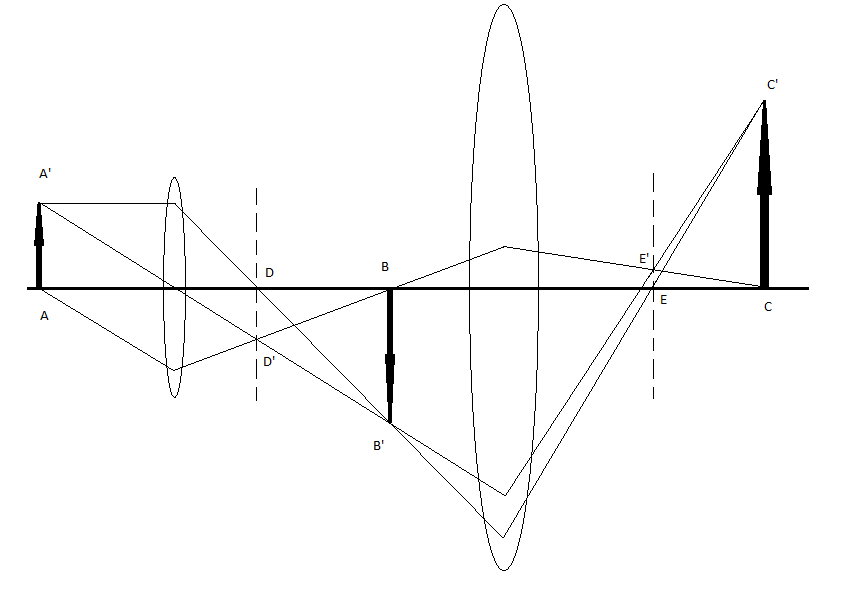
\includegraphics[width=\textwidth]{Strahlengang.png}
\caption{Schematische und vereinfachte Darstellung des Strahlenganges zur Entstehung der zwei Bildarten. Realbilder bei BB' und CC'. Beugungsbilder bei DD' und EE'.}
\label{Strahlengang}
\end{figure}
Werden Elektronen an den Atomen im Kristall gestreut, so ergibt sich eine vom Steuwinkel abhängige Intensitätsverteilung. Die Elektronen werden nach dem Bragg-Gesetz gestreut. Da die Winkel durch die kurze Wellenlänge der Elektronen jedoch sehr klein sind, kann der Bragg-Winkel genähert werden zu:
\begin{align}
2d\theta = n\lambda
\end{align}
Mit \(\lambda\) der Wellenlänge der Elektronen, \(d\) dem Abstand der Atome im Gitter und \(\theta\) dem Winkel des Elektronenstrahls zur Atomebene. Somit werden für jeden Gitterpunkt bestimmte Reflexe erwartet. Jedoch entstehen nicht von jedem Gitterpunkt Reflexe. Über den Strukturfaktor können nun die verbotenen und erlaubten Reflexe berechnet werden.
\begin{align}
F_\mathrm{hkl}= \sum_{j=1}^n f_\mathrm{j}(\theta)\exp[-2\pi i (hu_\mathrm{j}+kv_\mathrm{j}+lw_\mathrm{j})]
\end{align}
Mit \(h,k,l\) den Millerschen Indizes, \(f_\mathrm{j}(\theta)\) dem Streufaktor und \(j=1,2,3,...,n\) dem \(j\)ten Atom in der Einheitszelle am Ort \((u,v,w)\).\\
Das Ergebnis sind Beugungsbilder, die von der Kristallstruktur abhängig sind. Besteht eine Probe aus mehreren Kristallen mit unterschiedlicher Orientierung zueinander, so überlagern sich die jeweiligen Beugungsbilder.
Eine anschauliche Verdeutlichung des Bragg-Gesetzes ist die Ewald-Kugel (Abb. \ref{ewald}). Dabei wird in das reziproke Gitter des Kristalls der einfallende Elektronenstrahl mit der Länge \(1/\lambda\) auf einen gewählten Ursprungsreflex gezeichnet. Die Länge des Elektronenstrahls gibt den Radius eines Kreises, dessen Mittelpunkt der Anfang des Elektronenstrahls definiert. Alle Reflexe, die nun auf dem Kreis liegen und nach dem Strukturfaktor nicht verboten sind, sind im Beugungsbild erkennbar. Da die Intensitätsbreite des Bragg-Winkels von der Dicke der Probe mit \(1/t\) abhängt, weicht das reziproke Gitter auf und es sind keine Punkte mehr, sondern Linien. Somit sind auch Reflexe sichtbar, wenn die Ewaldkugel knapp die reziproken Gitterpunkte verfehlt.
\begin{figure}\center
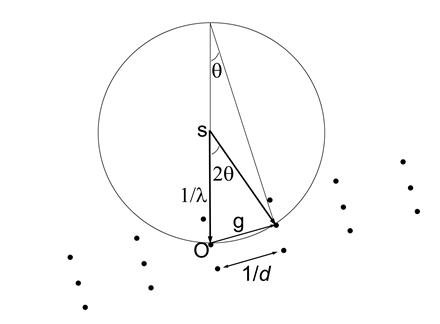
\includegraphics[width=0.65\textwidth]{ewald.png}
\caption{Konstruktion der Ewaldkugel im reziproken Kristallgitter.}
\begin{flushleft}
{\footnotesize Quelle: http://www.ammrf.org.au/myscope/tem/background/concepts/imagegeneration/diffraction/\\ewald/, 15.01.2018}
\end{flushleft}
\label{ewald}
\end{figure}
\\
Da selbst die elektromagnetischen Linsen keine perfekten Linsen sind, treten auch hier Fehler auf. Dies sind u.a. die sphärische Aberration, die chromatische Aberration und der Linsenastigmatismus. Die sphärische Aberration ist ein Phänomen bei dem die Strahlen, die am Rand der Linse auftreffen weiter entfernt fokussiert werden, als Strahlen, die auf die Mitte der Linse treffen. Dieser Fehler wird in neueren TEM's durch Mulitpolkorrektoren zu kleineren Werten korrigiert. Die Chromatische Aberration beschreibt die unterschiedliche Fokussierung von Elektronen mit unterschiedlichen Energien oder Wellenlängen. Da die aus dem Filament beschleunigten Elektronen nicht alle mit einer gleichen Energie austreten, sondern durch thermische Effekte einer gewissen Schwankung unterliegen, werden auch diese Elektronen unterschiedlich fokussiert. Der letzte signifikante Fehler ist der Linsenastigmatismus bei dem die Linse in x-Richtung und y-Richtung unterschiedlich stark fokussieren. Die Folge ist ein elliptischer und nicht kreisförmiger Elektronenstrahl. Dies kann durch Einstellung der Linsenspannungen korrigiert werden.
	
\section{Versuchsaufbau und Versuchsdurchführung}
Bei dem verwendeten Transmissionselektronenmikroskop handelt es sich um ein Titan 80/300. Es wird verwendet um an einer InGaAs/GaAs-Probe Beugungs- und Realbilder aufzunehmen. Die Probe wurde im FIB präpariert und auf eine Dicke von wenigen Nanometern geschnitten. Im TEM werden in einer Kathode Elektronen freigesetzt und mittels einer an die Lochanode angelegte Spannung von \(300\,\mathrm{kV}\) beschleunigt (Abb \ref{TEM}). Über ein System aus elektromagnetische Linsen werden die Elektronen auf die Probe fokussiert. Dort werden sie teilweise an den Atomen im Kristallgitter gestreut nach dem Bragg-Gesetz und teilweise reflektiert. Auch werden Elektronen aus den inneren Energieniveaus herausgeschlagen. Wodurch Elektronen aus höheren Energieniveaus in das entstandene Loch zurückfallen und ihre überschüssige Energie als elektromagnetische Strahlung abgeben. Dies ist die charakteristische Röntgenstrahlung und kann auch über ein EDX-System analysiert werden. Dies erlaubt die Bestimmung des Materials.
Die gestreuten Elektronen werden transmittiert und werden wiederum über ein Linsensystem fokussiert. Die Elektronen treffen nun auf einen Beobachtungsschirm, oder eine CCD-Kamera. Über eine weitere Linse wird nun der Strahlengang so gelegt, dass entweder das Beugungsbild, oder das Abbildungsbild zuerkennen ist. Der gesamte Strahlengang befindet sich im Hochvakuum, sodass unerwünschte Wechselwirkungen der Elektronen mit der Luft verhindert werden.

\begin{figure}[H]
\center
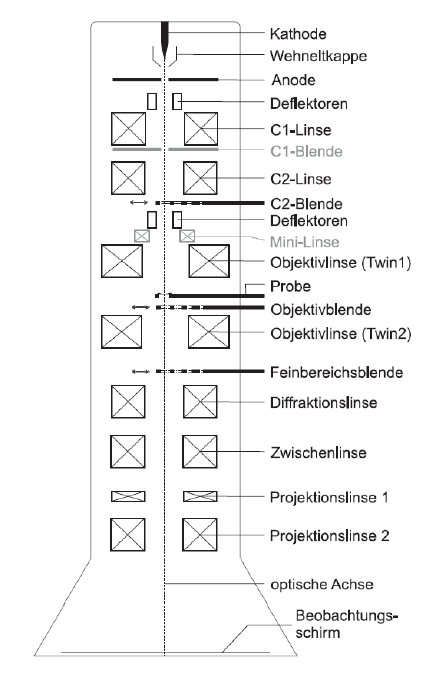
\includegraphics[width=0.6\textwidth]{tem.png}
\caption{Schematischer Aufbau eines Transmissionselektronenmikroskop. Die aus der Kathode beschleunigten Elektronen werden über mehrere Linsen- und Blendensysteme auf die Probe fokussiert. Nach der Transmission werden die Elektronen erneut auf einen Beobachtunsschirm, oder eine Kamera fokussiert.}
\begin{footnotesize}
\begin{flushleft}
Quelle: Versuchsanleitung FP16: Fortgeschrittenenpraktikum Transmissionselektronenmikroskopie
\end{flushleft}
\end{footnotesize}
\label{TEM}
\end{figure}

Bevor das Beugungsbild einer Probe aufgenommen werden kann, muss das TEM zuerst justiert werden. Dazu wird der Elektronenstrahl auf eine freie Stelle fokussiert, an der er die Probe nicht trifft. Als erstes wird die C2-Blende zentriert, sodass bei einem Vergrößerungswechsel der Strahl in der Mitte des Schirms bleibt. Danach wird der Elektronenstrahl auf eine kreisrunde Form gebracht, da dieser durch den Kondensorastigmatismus zumeist elliptisch ist. Als dritter Schritt wird der Strahl auf die Probenoberfläche fokussiert und anschließend wird das Rotationszentrum durch eine periodische Anregung der Objektivlinse eingestellt. Nach der Justage werden Beugungsbilder aufgenommen, sowohl in Zonenachse, als auch mit anderen Lauekreiszentren. Danach werden Aufnahmen im Abbildungsmodus von den InGaAs-Quantentrögen gemacht, wobei Hellfeldaufnahmen mit dem Reflex (000), aber auch Dunkelfeldaufnahmen mit den Reflexen (022) und (004) gemacht werden. Durch weitere hochaufgelöste Aufnahmen im Hellfeld Abbildungsmodus der Quantentröge werden im Anschluss einmal über den Gitterabstand und einmal über den Intensitätsverlauf der Indiumgehalt bestimmet. Da die Gittkonstanten von GaAs und InAs unterschiedlich sind, wird es zu einer Verzerrung des Gitters in einem Mischkristall kommen. Diese Verzerrung ist dann natürlich von der Konzentration an Indiumatomen abhängig. Die andere Möglichkeit über den Intensitätsverlauf zielt darauf ab, dass der Strukturfaktor ebenfalls linear von der Konzentration an Indiumatomen abhängt. Die Intensität ist nun proporional zum Betragsquadrat des Strukturfaktors. So kann über eine Normierung an Punkten ohne Indium aus der Intensität auf die Konzentration der Indiumatome geschlossen werden.

\section{Auswertung}

Es wurde eine GaAs Probe untersucht, die Quantentröge aus InGaAs enthält. Auf einem Bereich mit mehreren solchen Quantentrögen wurde das Beugungsbild in Abb. \ref{100ind} aufgenommen, während die Probe in Zonenachse [100] orientiert war.

\begin{figure}[h]\centering
	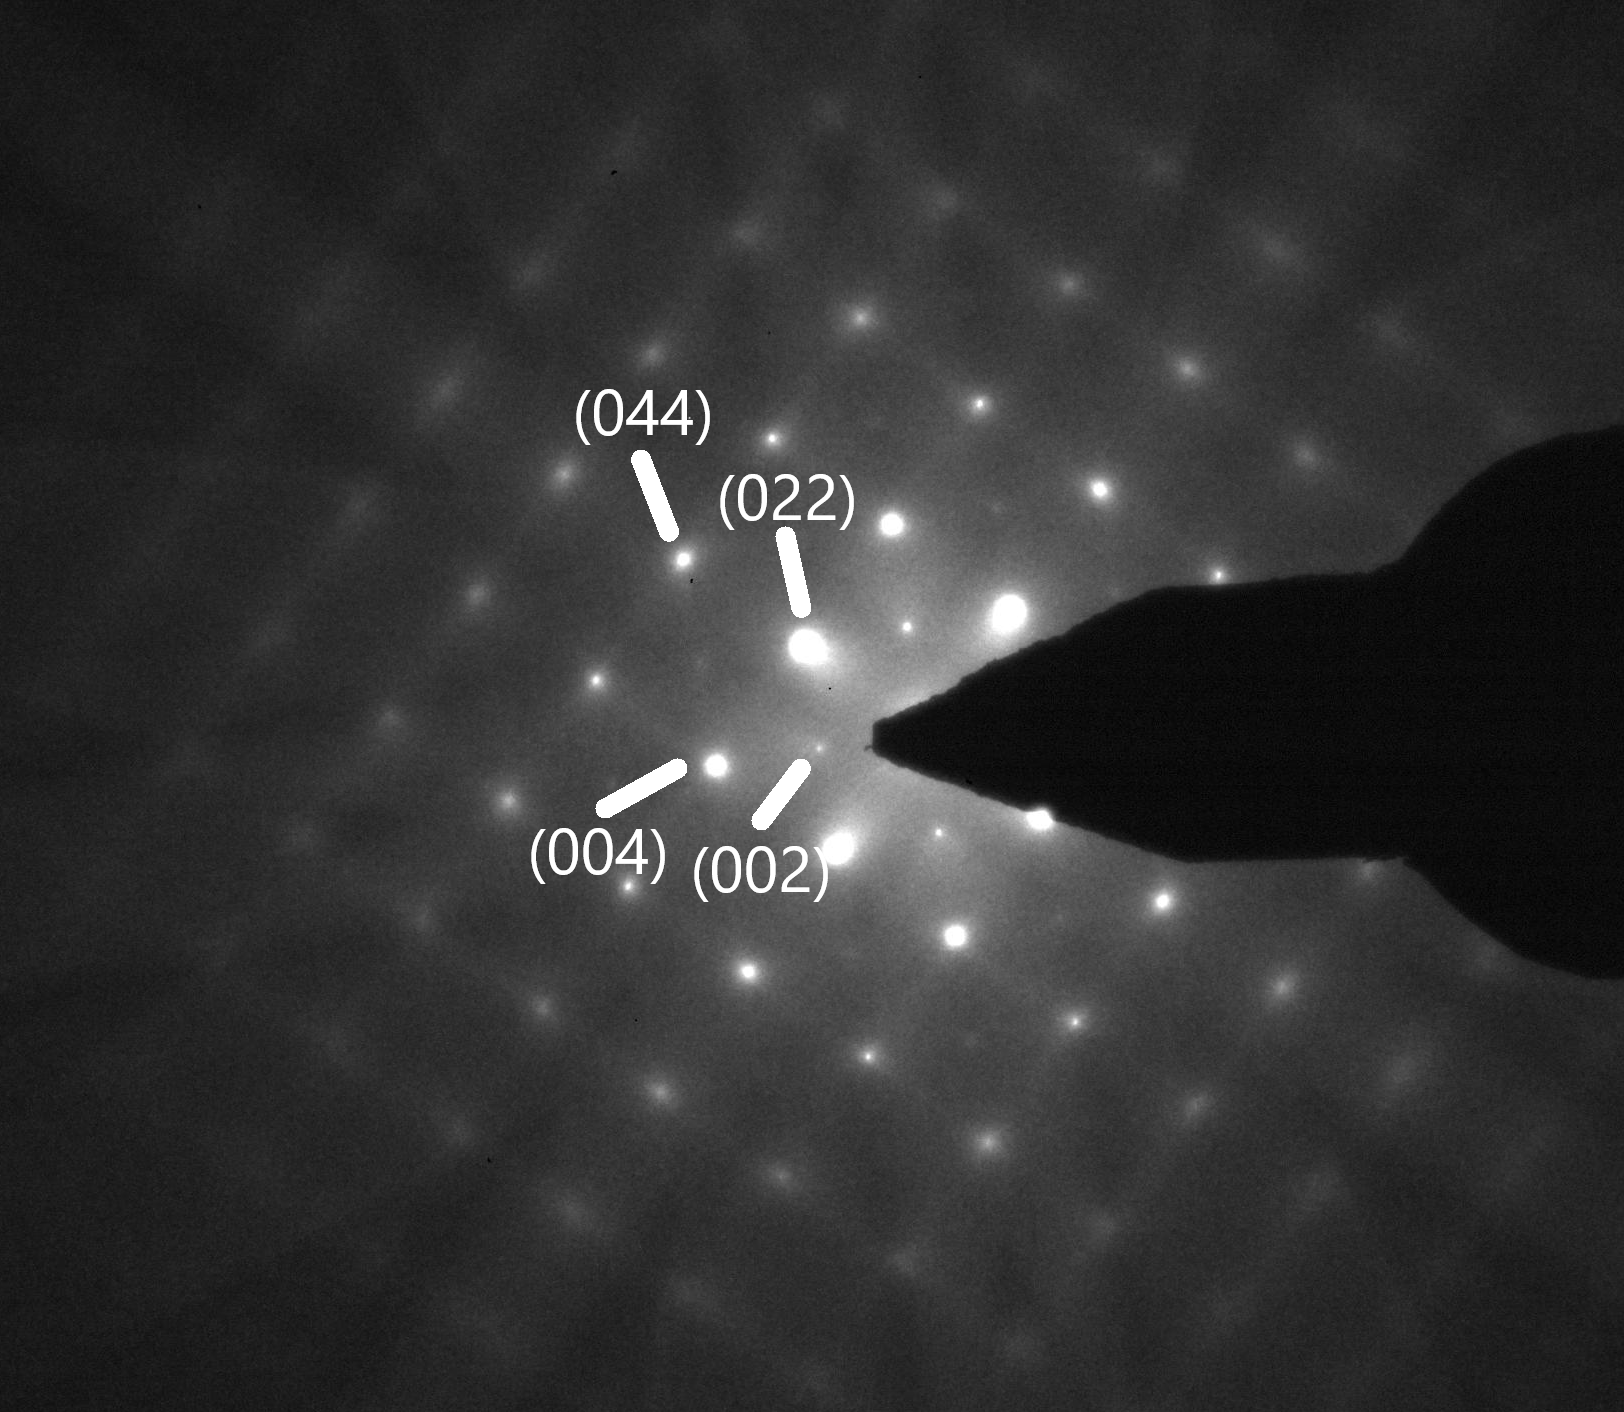
\includegraphics[width=0.65\textwidth]{Versuchsdaten/8/indiziert2.png}
\caption{Beugungsbild auf GaAs in Zonenache [100]}
\label{100ind}
\end{figure}

Die Zonenachse [100] ist dadurch zu erkennen, dass der Reflex (000) in der Mitte des Lauekreises liegt. Wird die Probe verkippt, bilden sich Lauekreise mit Zentren abseits des Punktes (000), sodass der Punkt (000) immer auf dem Rand des Kreises liegt. Da GaAs ein kubischflächenzentriertes Gitter mit zwei Atomsorten bildet, haben alle Punkte mit ungeraden Laue-Indizes einen Strukturfaktor von 0. Dementsprechend sind die entsprechenden Reflexe auf dem Beugungsbild auch nicht zu erkennen. Die Helligkeitsverteilung entspricht dabei den Erwartungen gemäß des Strukturfaktors. Gallium sitzt an den Gitterplätzen [0 0 0], [0 $\frac{1}{2}$ $\frac{1}{2}$], [$\frac{1}{2}$ 0 $\frac{1}{2}$] und [$\frac{1}{2}$ $\frac{1}{2}$ 0]. Somit erhält der Strukturfaktor nur einen Wert für ganze Laue-Indizes. Um zu erklären, dass der Reflex (004) heller ist, als (002), muss der Strukturfaktor vom Arsen angesehen werden. Die Arsen-Atome sitzen um [$\frac{1}{4}$ $\frac{1}{4}$ $\frac{1}{4}$] verschoben zu den Gallium-Atomen. Dies hat zur Auswirkung, dass der Strukturfaktor von Arsen nur ungleich 0 ist für Laue-Indizes, dessen Summe ein ganzes Vielfaches von 4 ist. Auf die etnsprechenden Reflexe, z.B. (004), (022), wirken sich somit die Streuamplituden beider Atome aus.
Im Folgenden wurden mehrere Beugungsbilder mit Lauekreiszentren (0 0 8),(0 2 2), (0 0 10), (0 $\bar{6}$ $\bar{2}$) und (0 0 2) aufgenommen.

\begin{figure}[htb]\centering
	\subcaptionbox{Beugungsbild mit Lauekreiszentrum (008)\label{008}}
	[.49\linewidth]{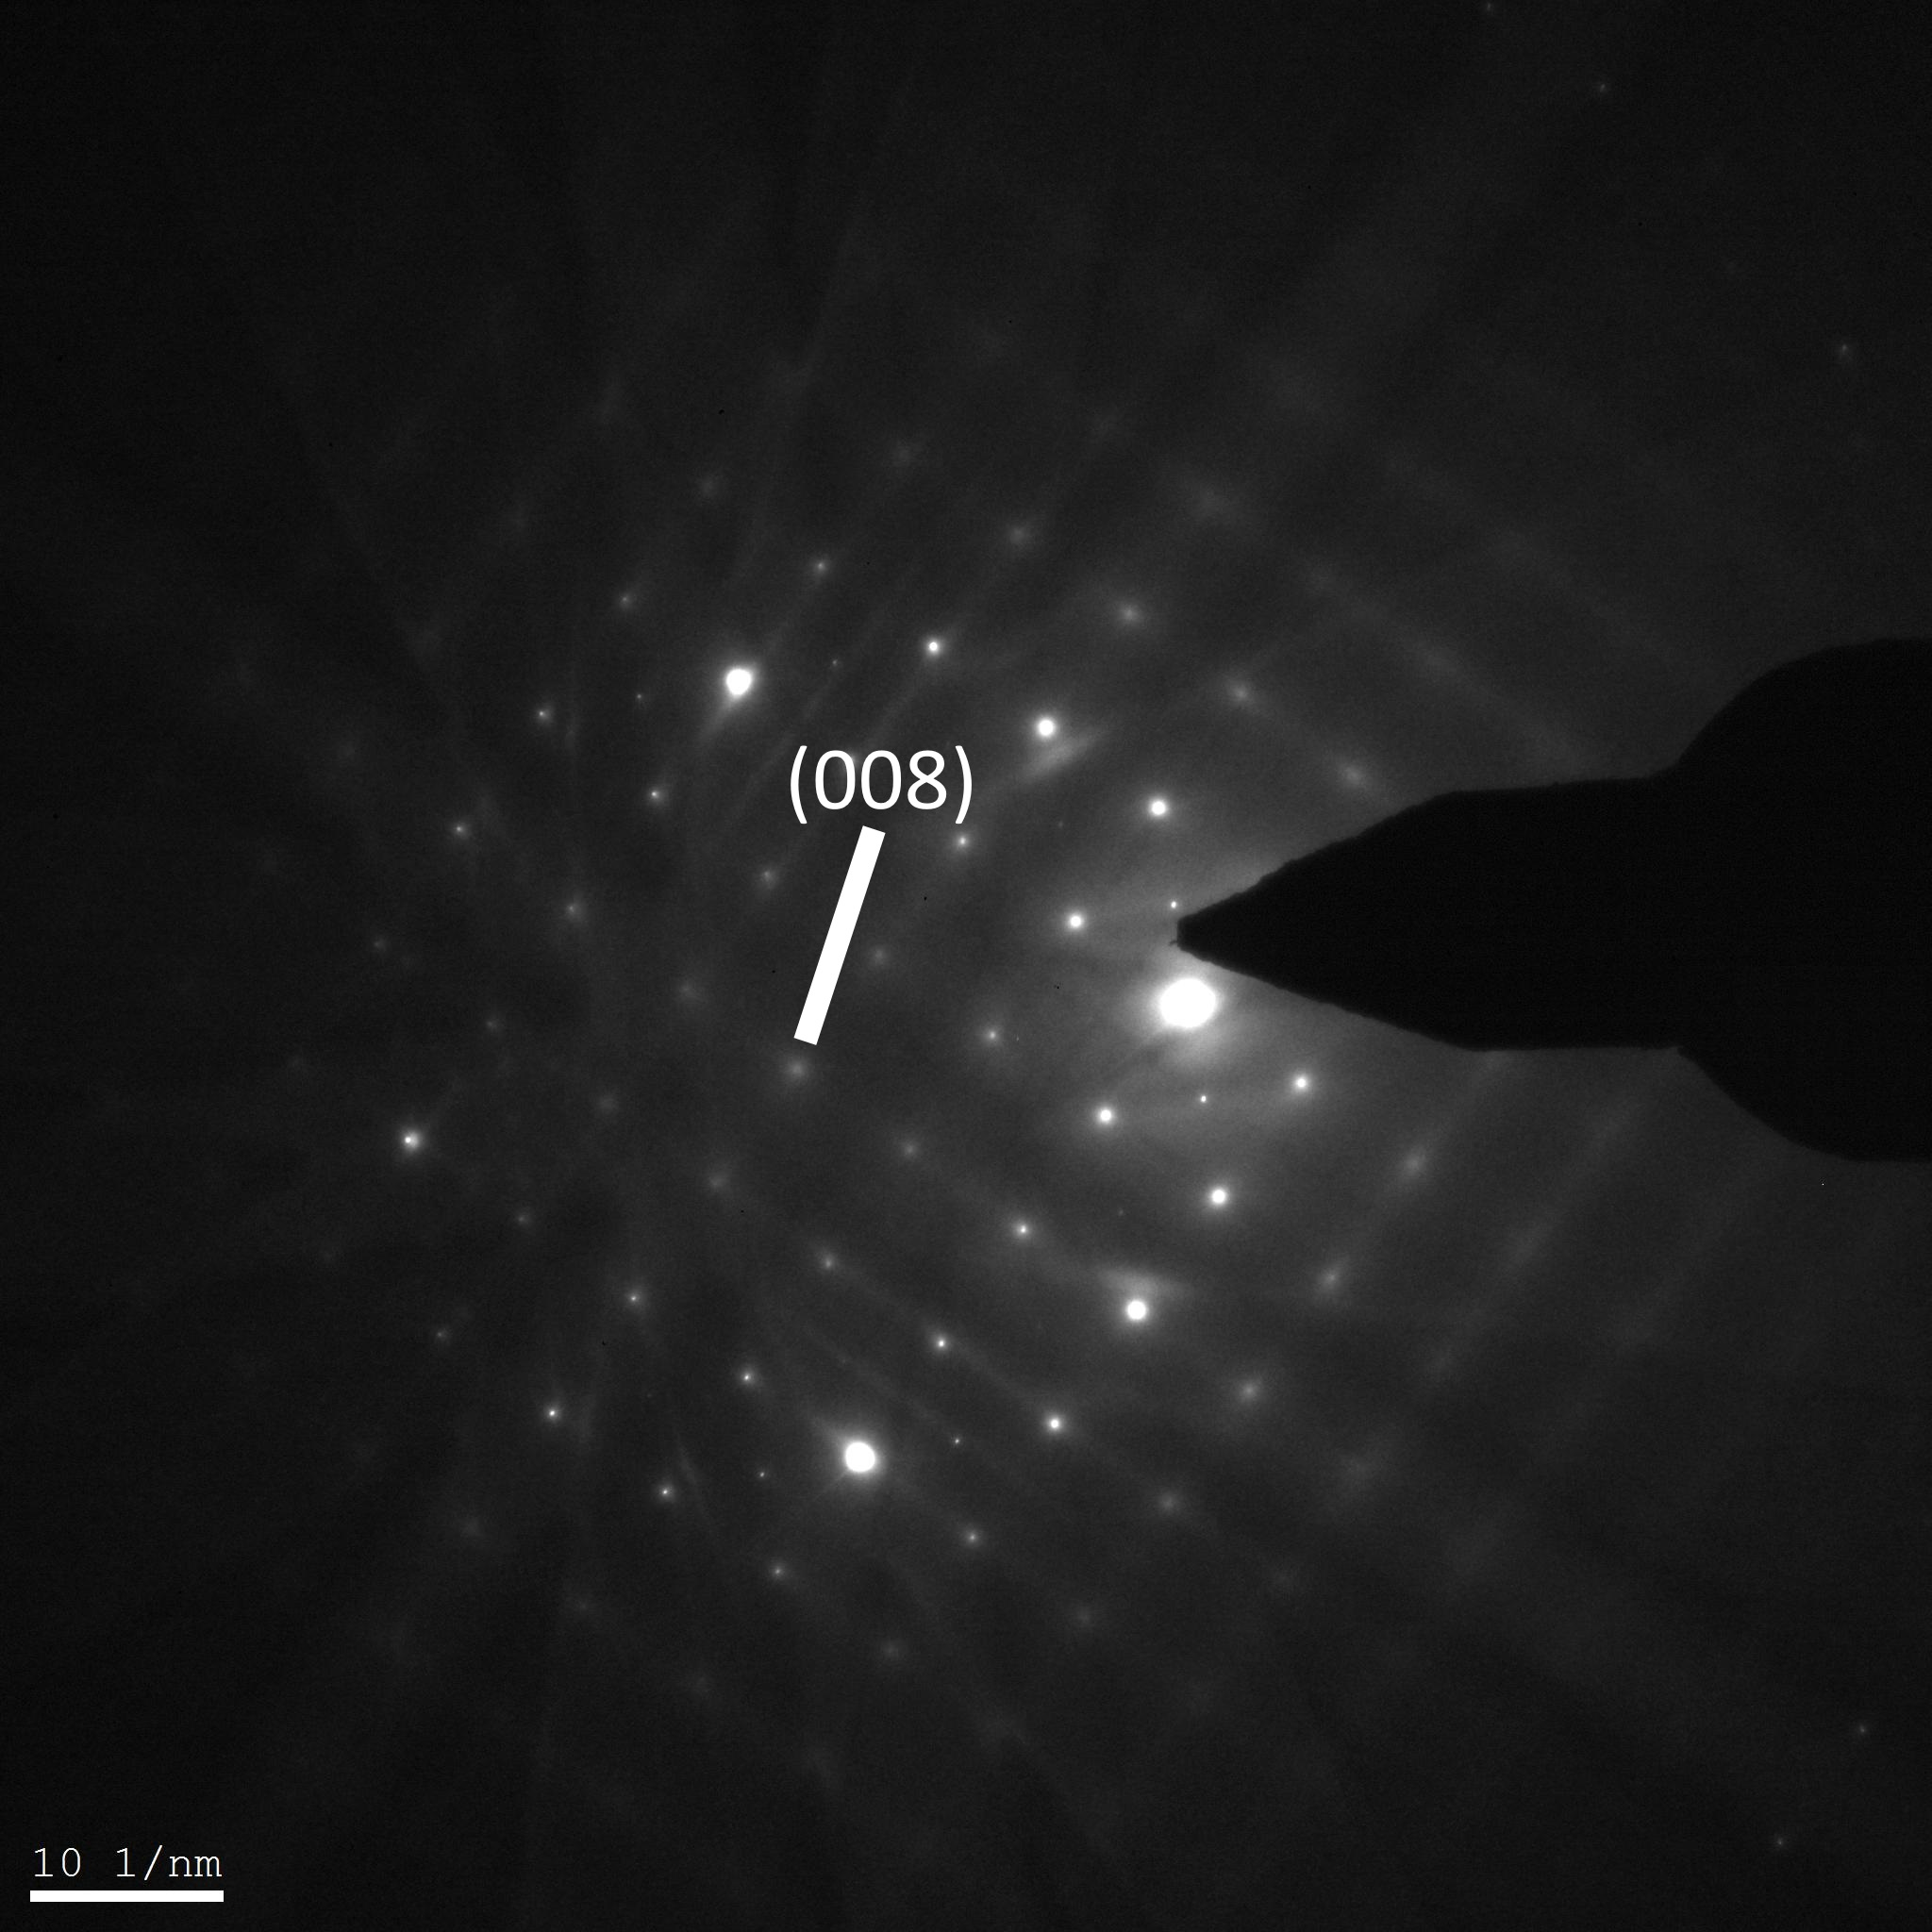
\includegraphics[width=0.49\textwidth]{Versuchsdaten/9/008.jpg}}
	\subcaptionbox{Beugungsbild mit Lauekreiszentrum (022)\label{022}}
	[.49\linewidth]{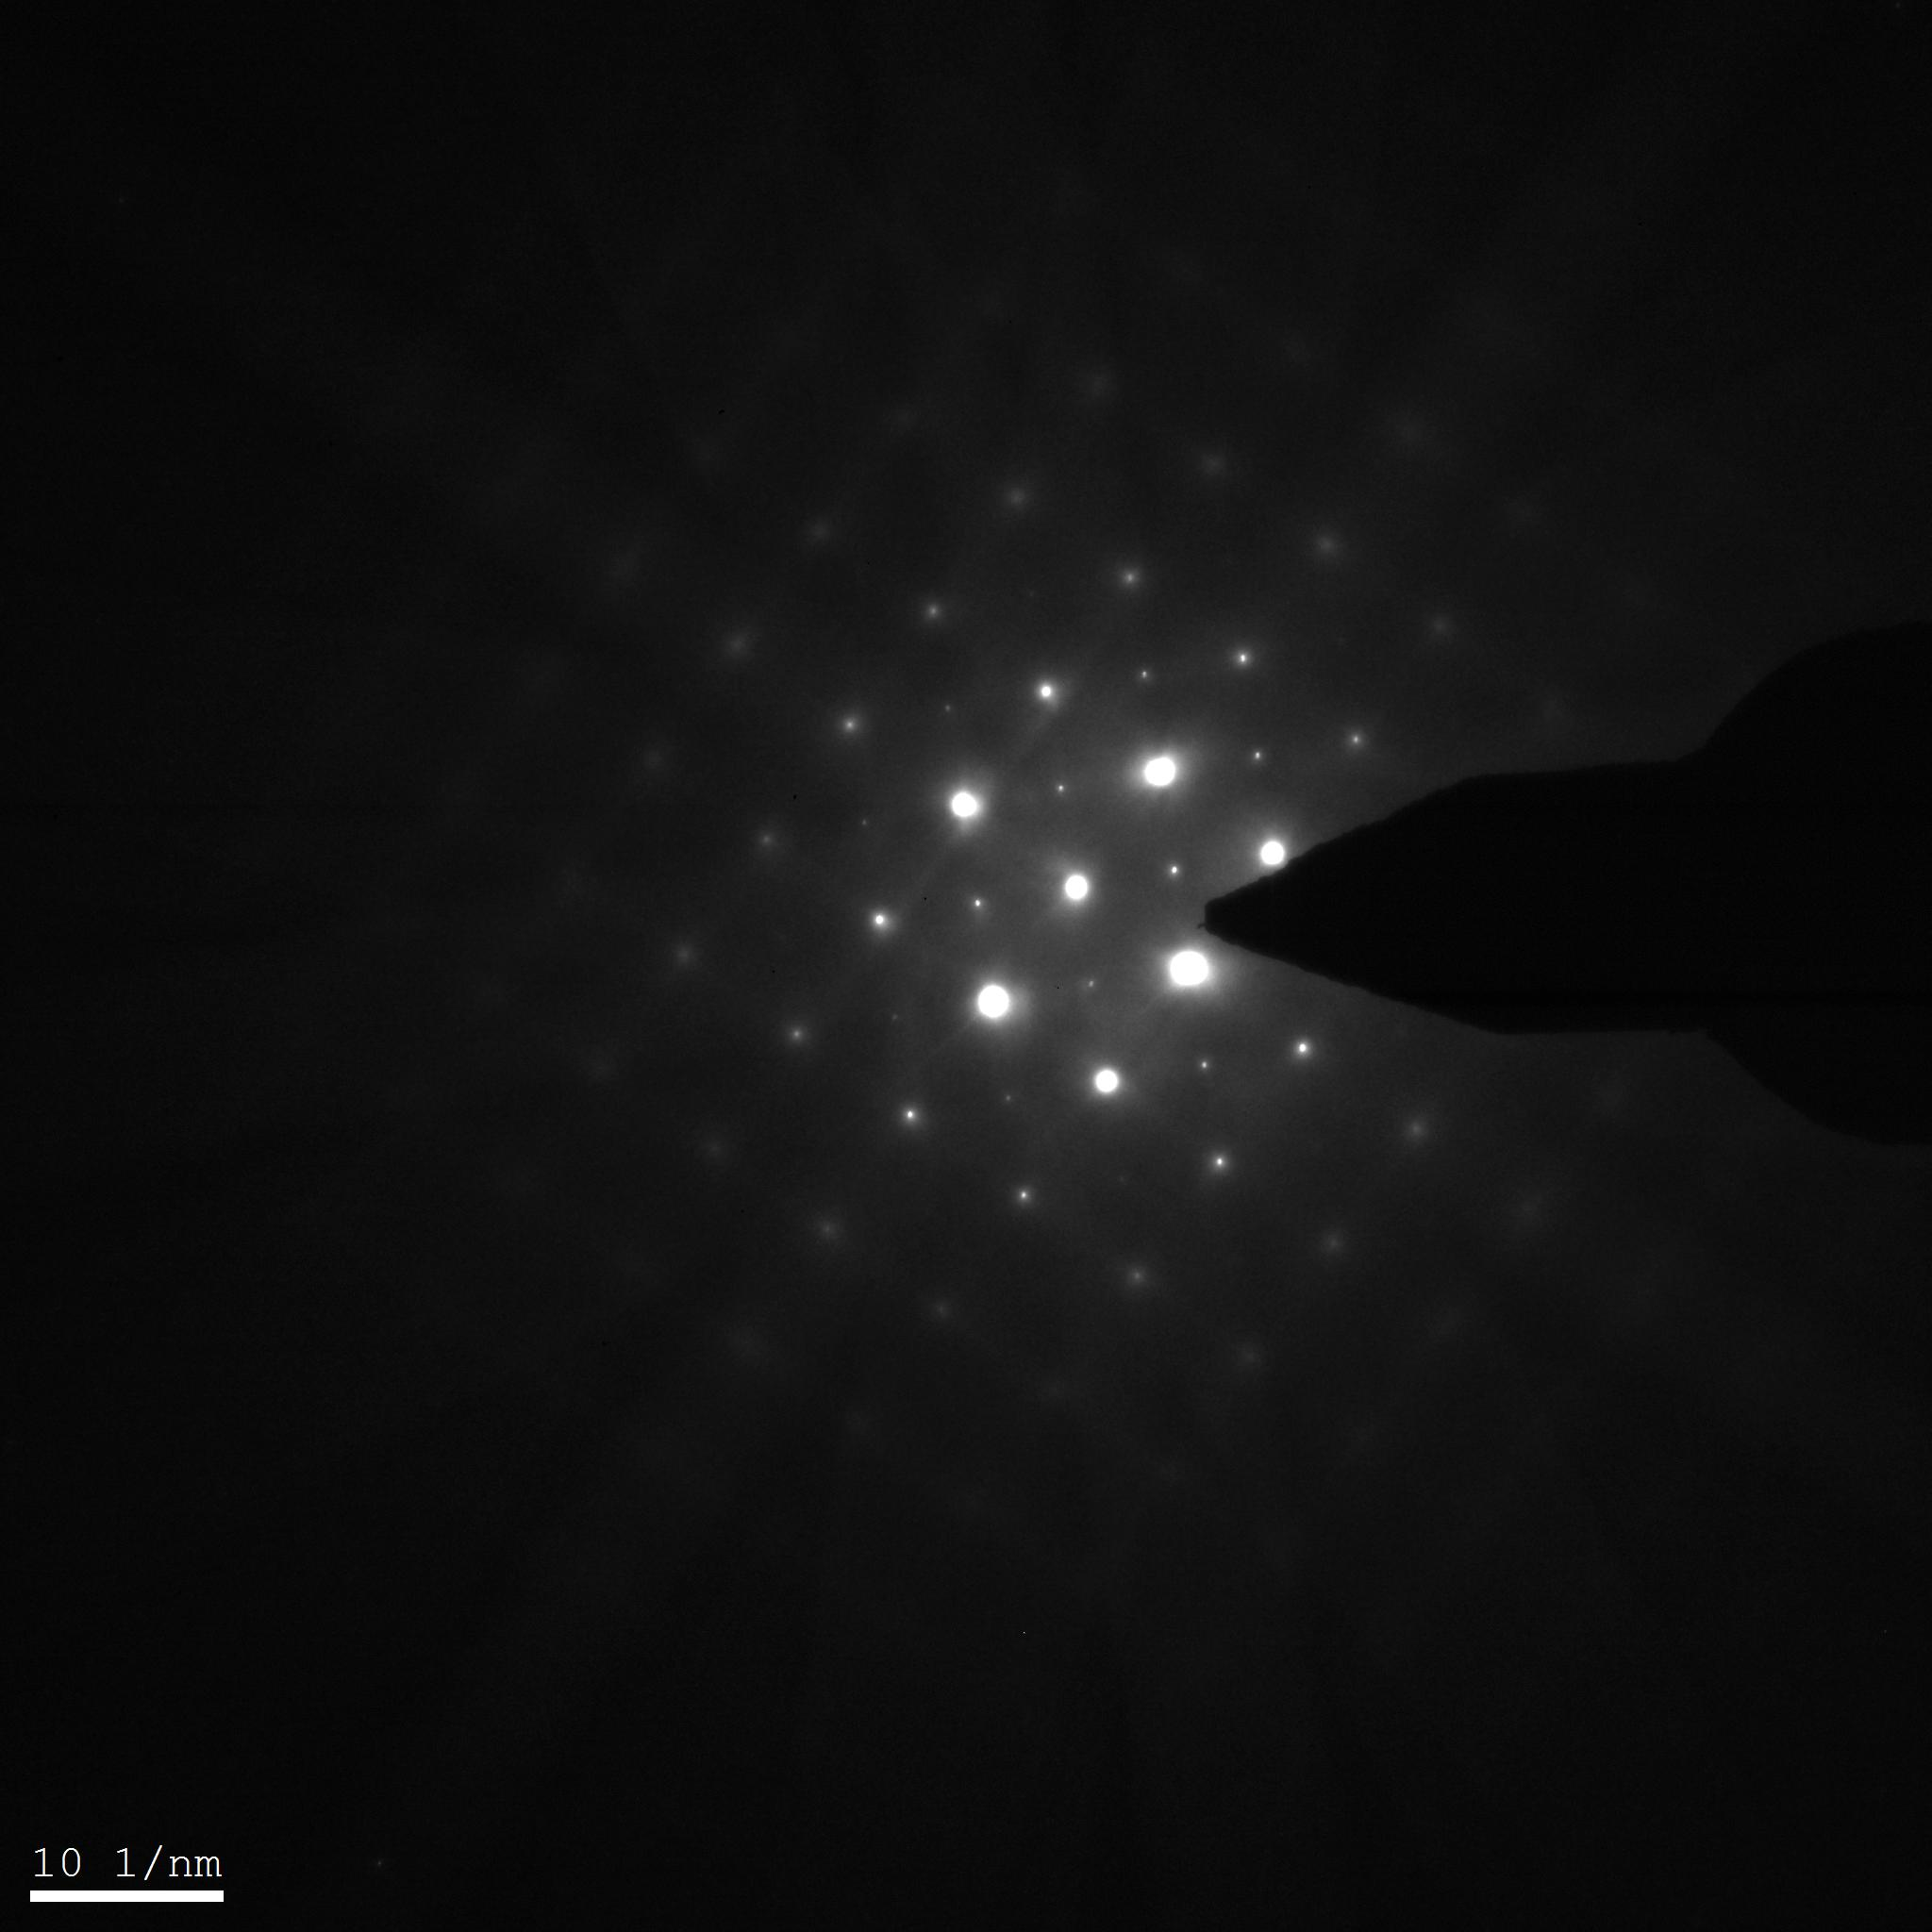
\includegraphics[width=0.49\textwidth]{Versuchsdaten/9/022.jpg}}\\
	\caption{Beugungsbilder bei unterschiedlichen Probendrehung} \label{laue1}
\end{figure}

In den Abb. \ref{008} und \ref{022} sind diese Beugungsbilder zu sehen. Im Lauekreis um das jeweilige Zentrum herum haben diejenigen Reflexe eine starke Intensität, die die Bragg-Reflexionsbedingung erfüllen. Eine Verschiebung des Lauekreiszentrums entsteht zudem auf unterschiedlichen Probenstellen durch geringe Unebenheiten oder auch durch anders ausgerichtete Kristallebenen erfolgen. \\
Es sind als Beispiel noch zwei Beugungsbilder mit zufälligen Lauekreiszentren aufgenommen wurden.

\begin{figure}[htb]\centering
	\subcaptionbox{Lauekreiszentrum (0 0 10)\label{rand}}
	[.49\linewidth]{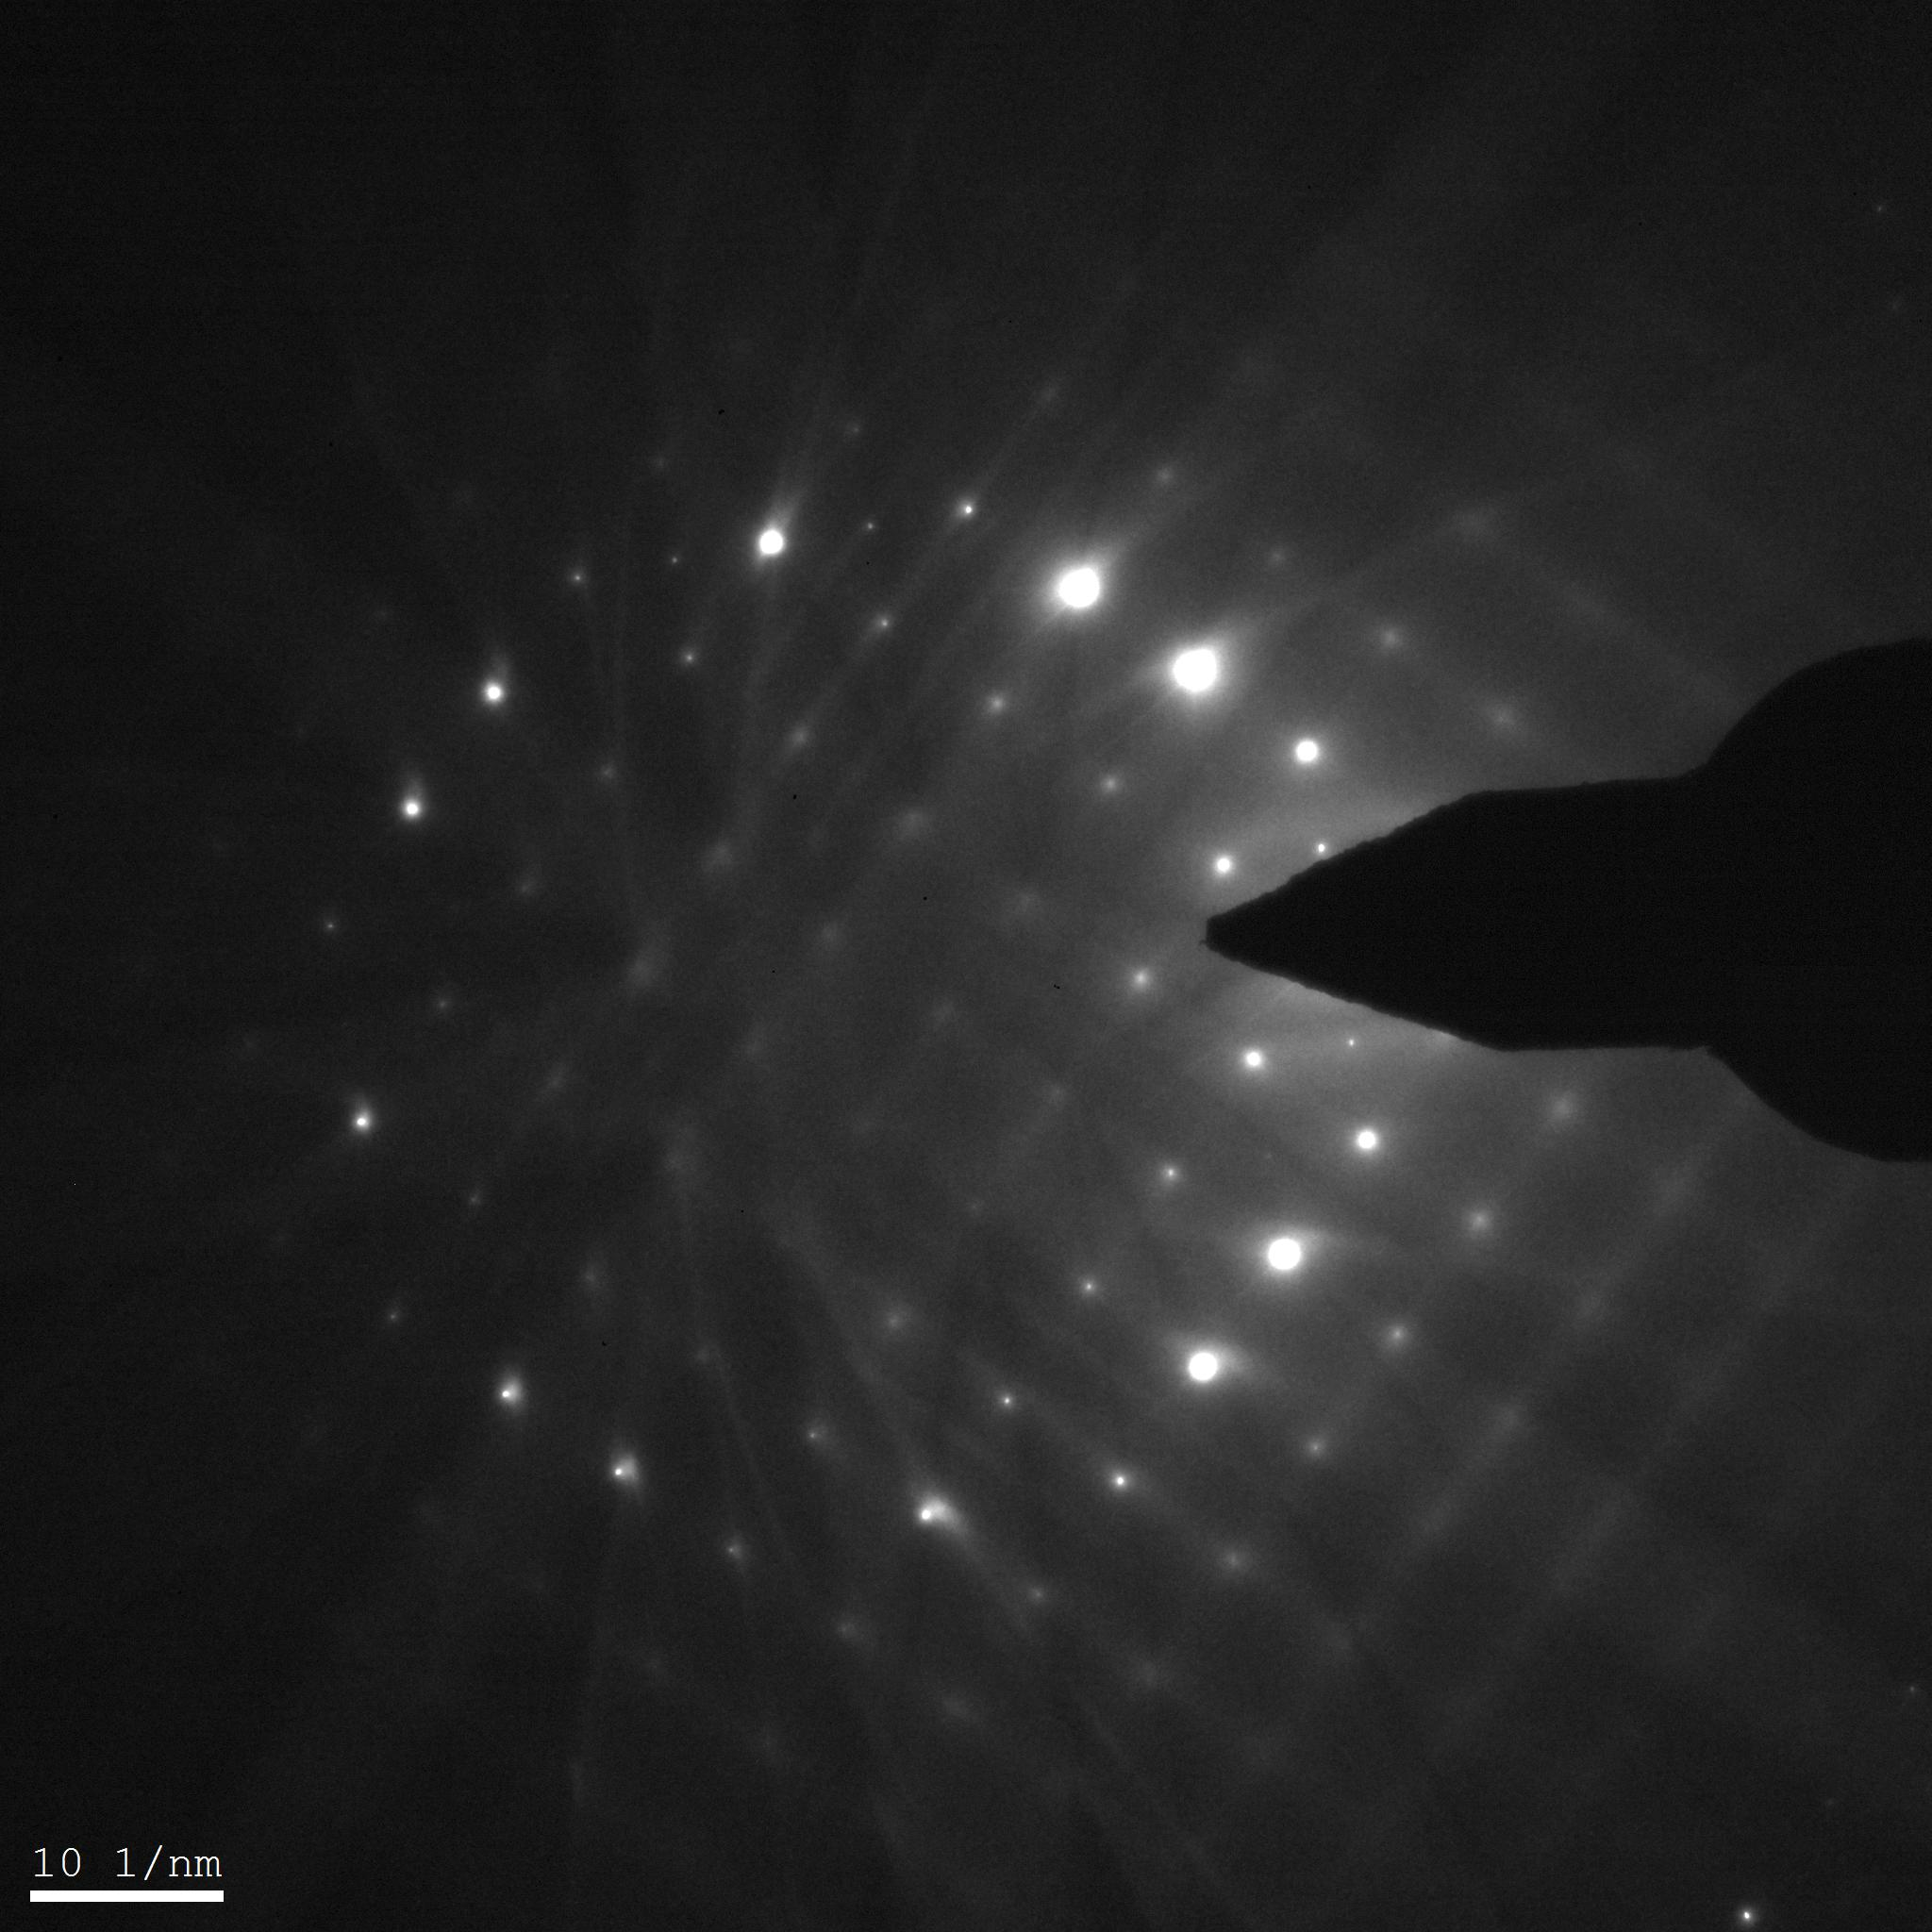
\includegraphics[width=0.49\textwidth]{Versuchsdaten/9/RandomTilt.jpg}}
	\subcaptionbox{Beugungsbild mit sichtbarem zweiten Lauekreis und Lauekreiszentrum bei (0 $\bar{6}$ $\bar{2}$)\label{rand1}}
	[.49\linewidth]{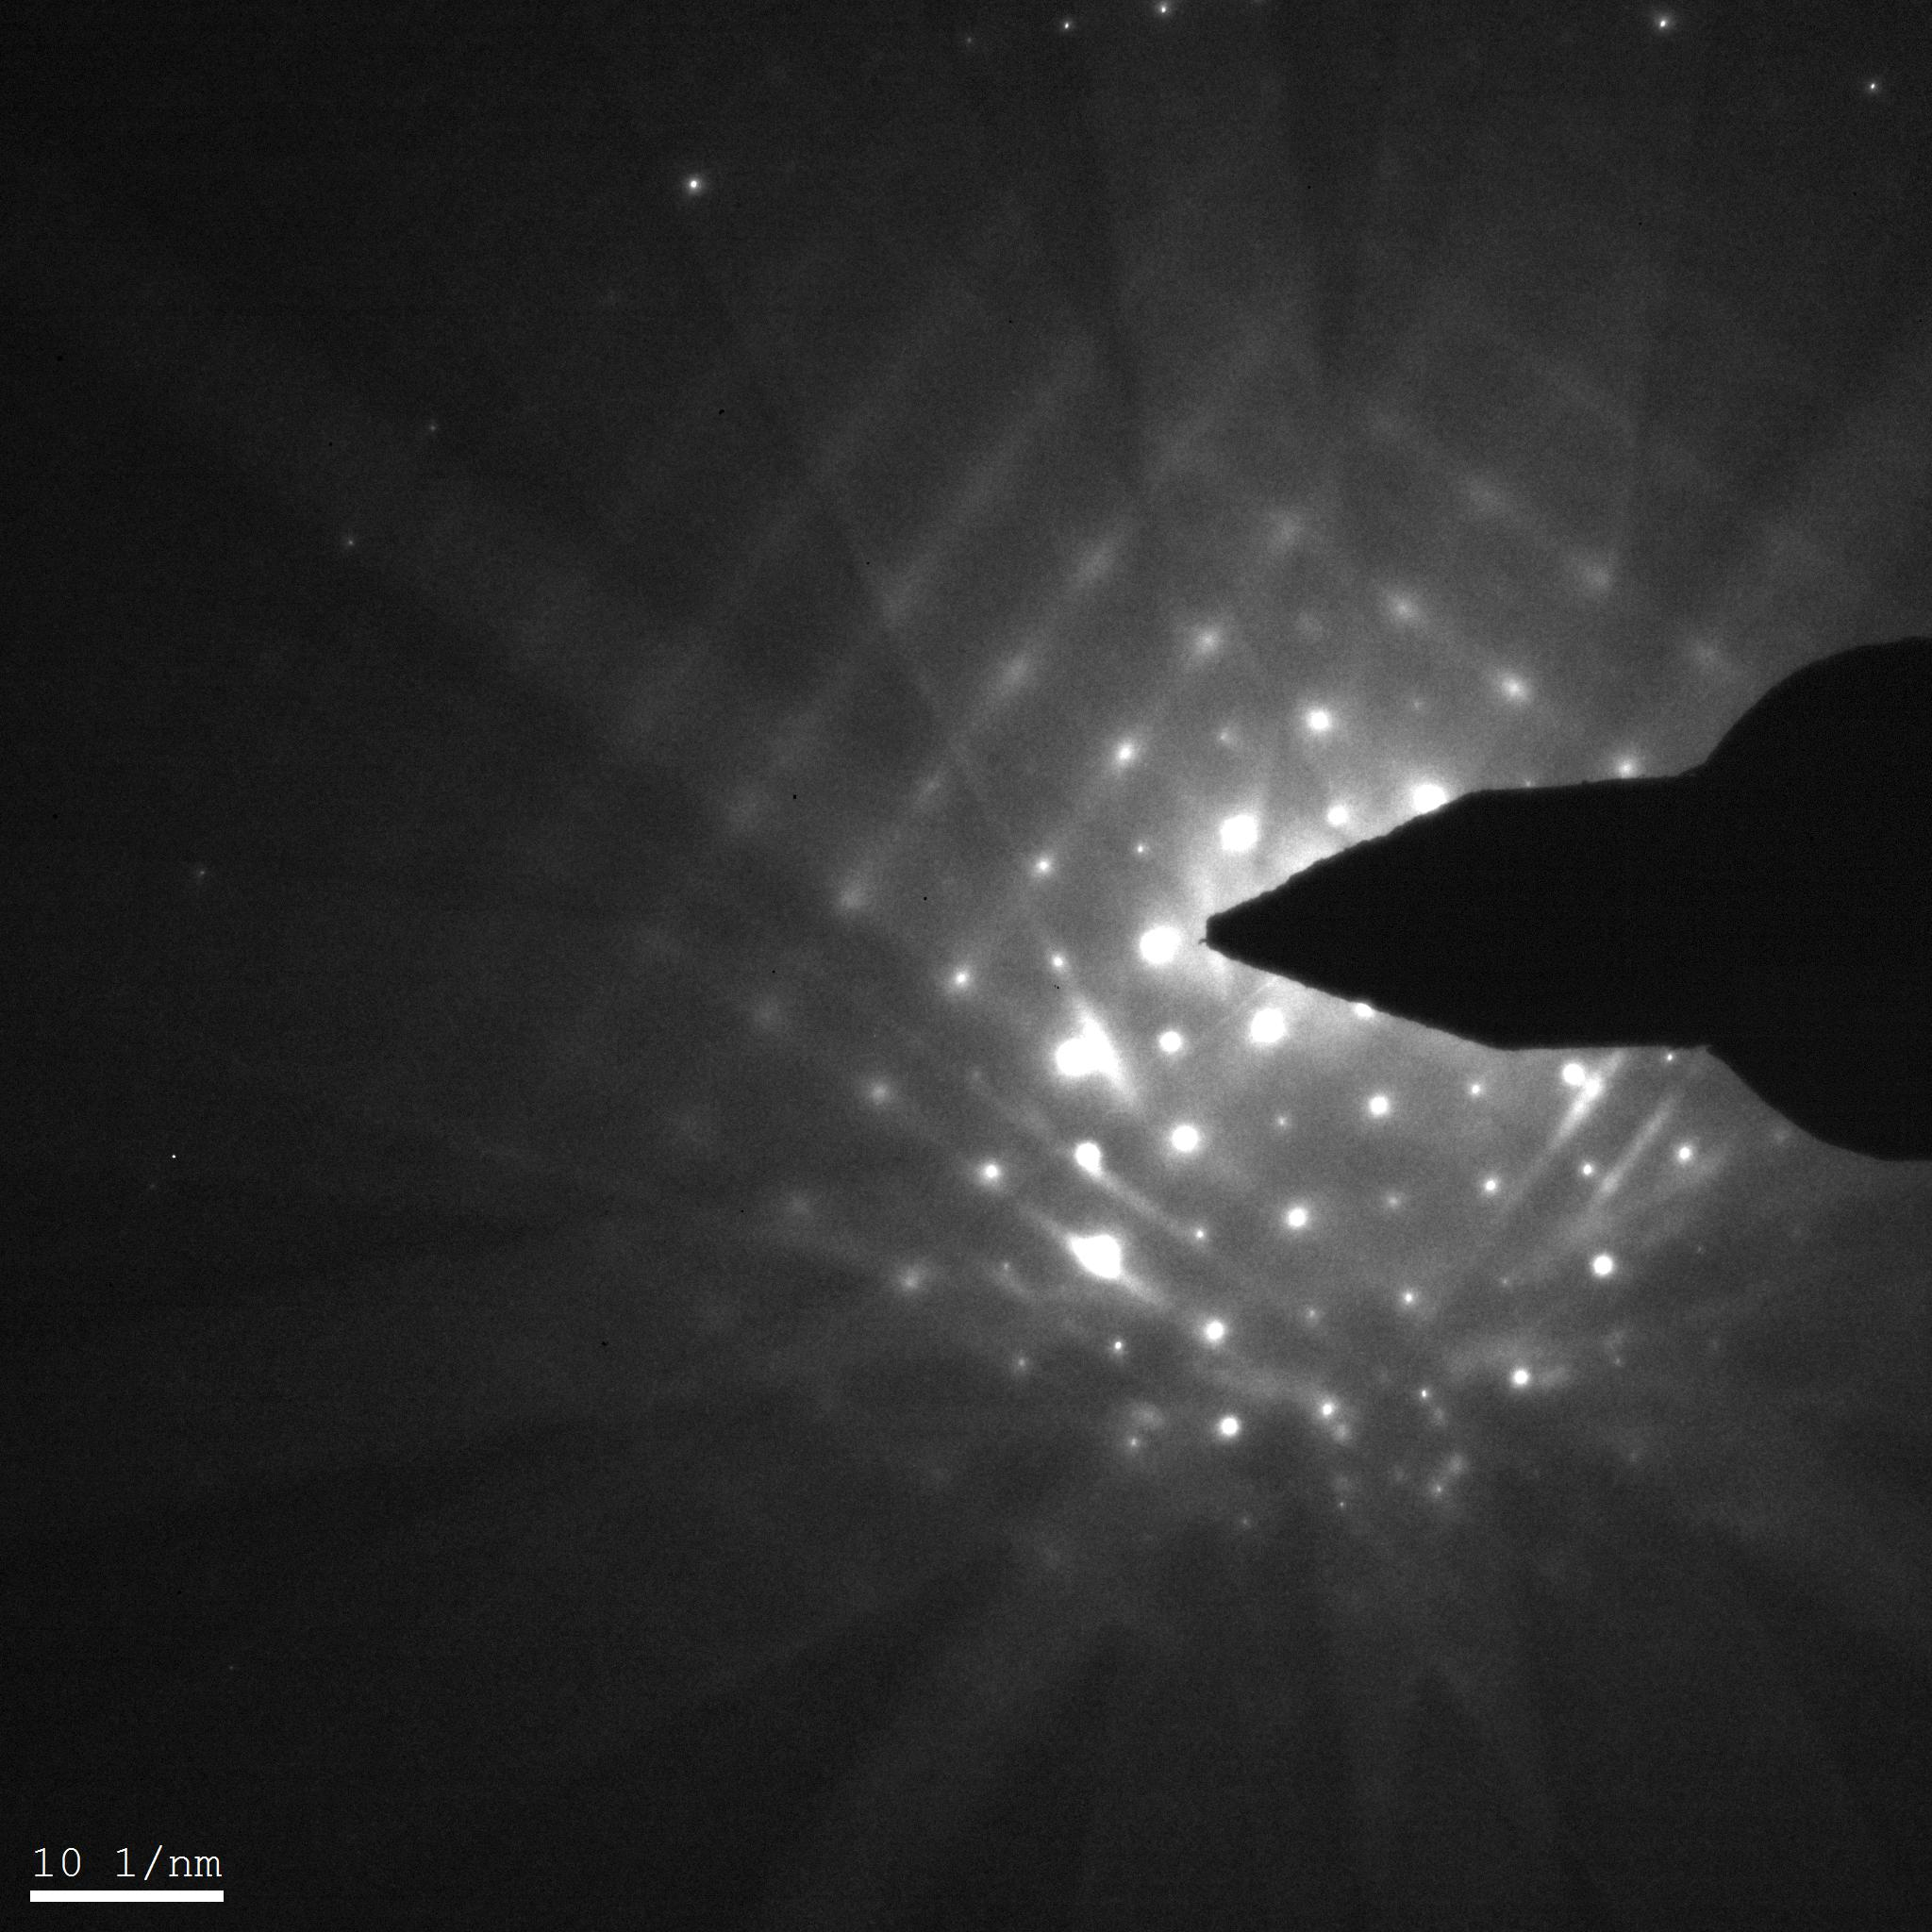
\includegraphics[width=0.49\textwidth]{Versuchsdaten/9/RandomTilt1.jpg}}\\
	\caption{Zwei Beugungsbilder mit zufälliger Drehung der Probe} \label{rands}
\end{figure}

Auf diese Weise ist Abb. \ref{rand} entstanden, in der deutlich die intensitätsreicheren Reflexe auf dem Lauekreis zu sehen sind. In Abb. \ref{rand1} ist zudem auch der zweite Lauekreis vor allem oberhalb des (000) Reflexes zu erkennen. \\
Damit die (004) Netzebenen in Bragg-Reflexionsstellung sind, muss der (004) Reflex im Beugungsbild auf dem Lauekreis liegen. Dies ist im einfachsten Fall beim Lauekreiszentrum (002) gegeben. Zu sehen ist dieser Fall in Abb. \ref{002} zu sehen.

\begin{figure}[H]\centering
	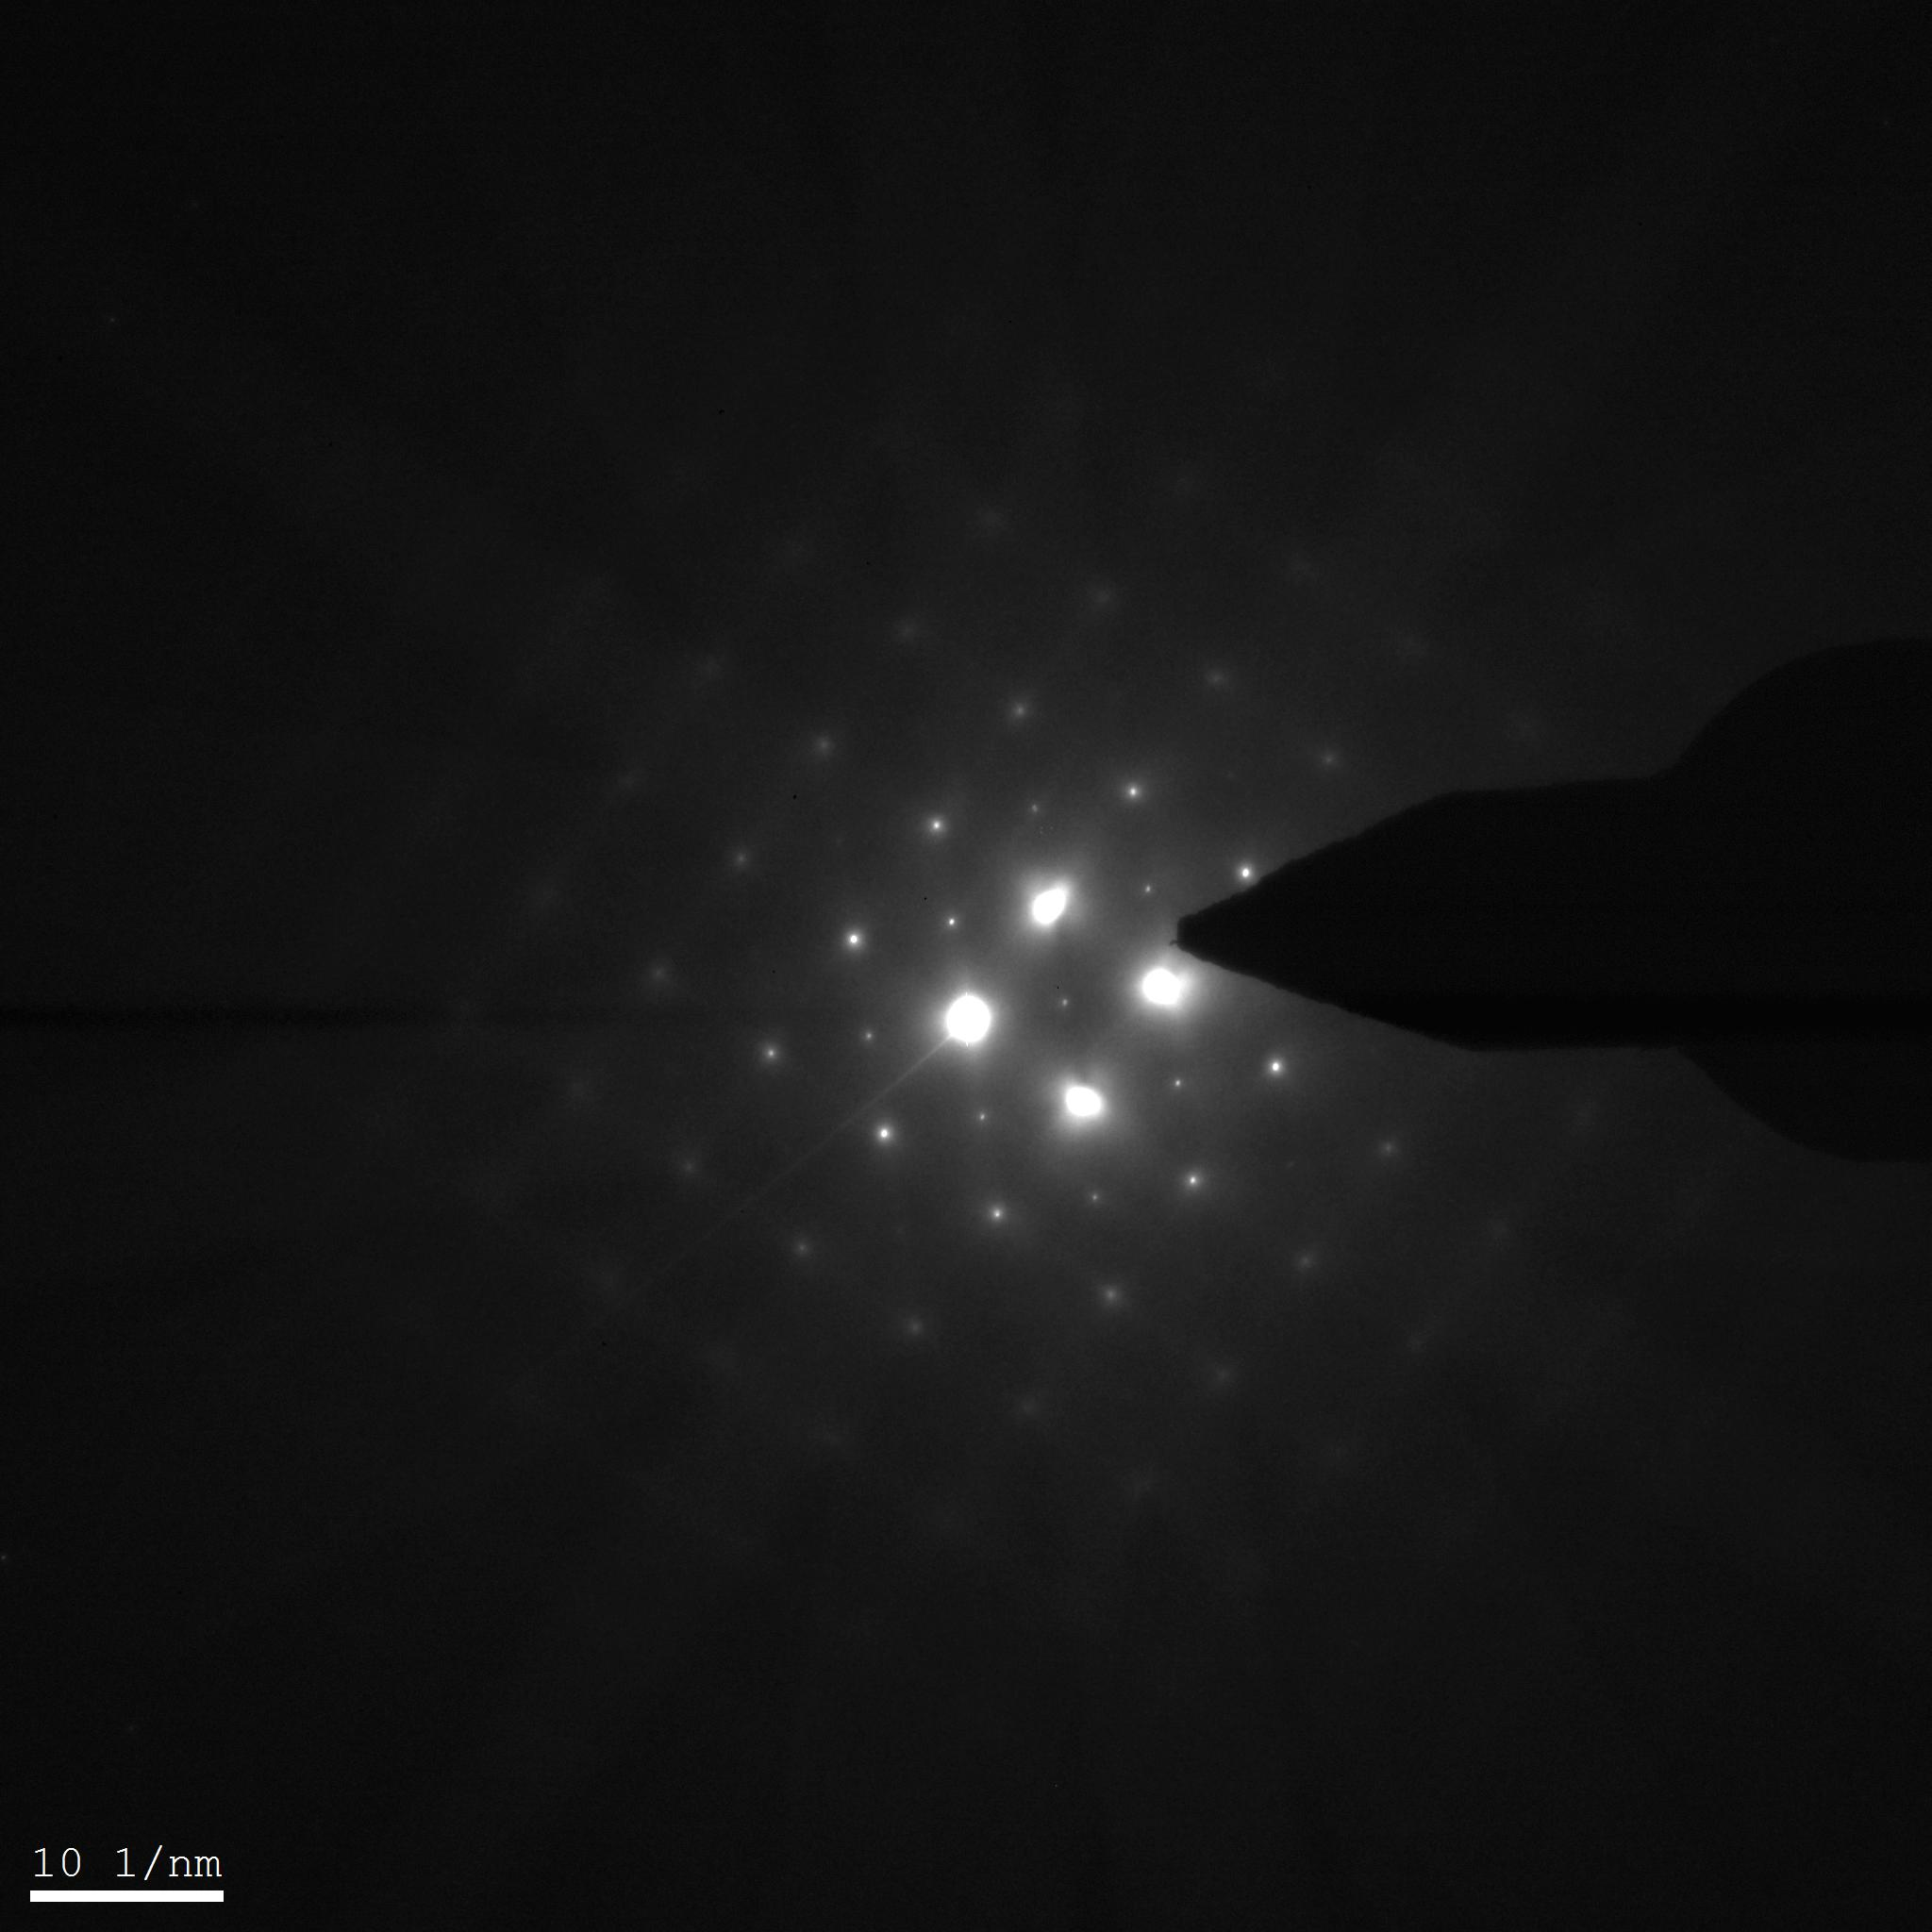
\includegraphics[width=0.65\textwidth]{Versuchsdaten/9/002.jpg}
\caption{Beugungsbild mit Lauekreiszentrum (002)}
\label{002}
\end{figure}

\newpage

Zudem liegt der Reflex (022) in diesem Fall ebenfalls auf dem Lauekreis. Indem mit einer kleinen Blende alle Reflexe bis auf einen ausgeblendet werden, konnten im Folgenden Dunkelfeldaufnahmen der Probe gemacht werden.

\begin{figure}[htb]\centering
	\subcaptionbox{Hellfeldaufnahme\label{hell}}
	[.32\linewidth]{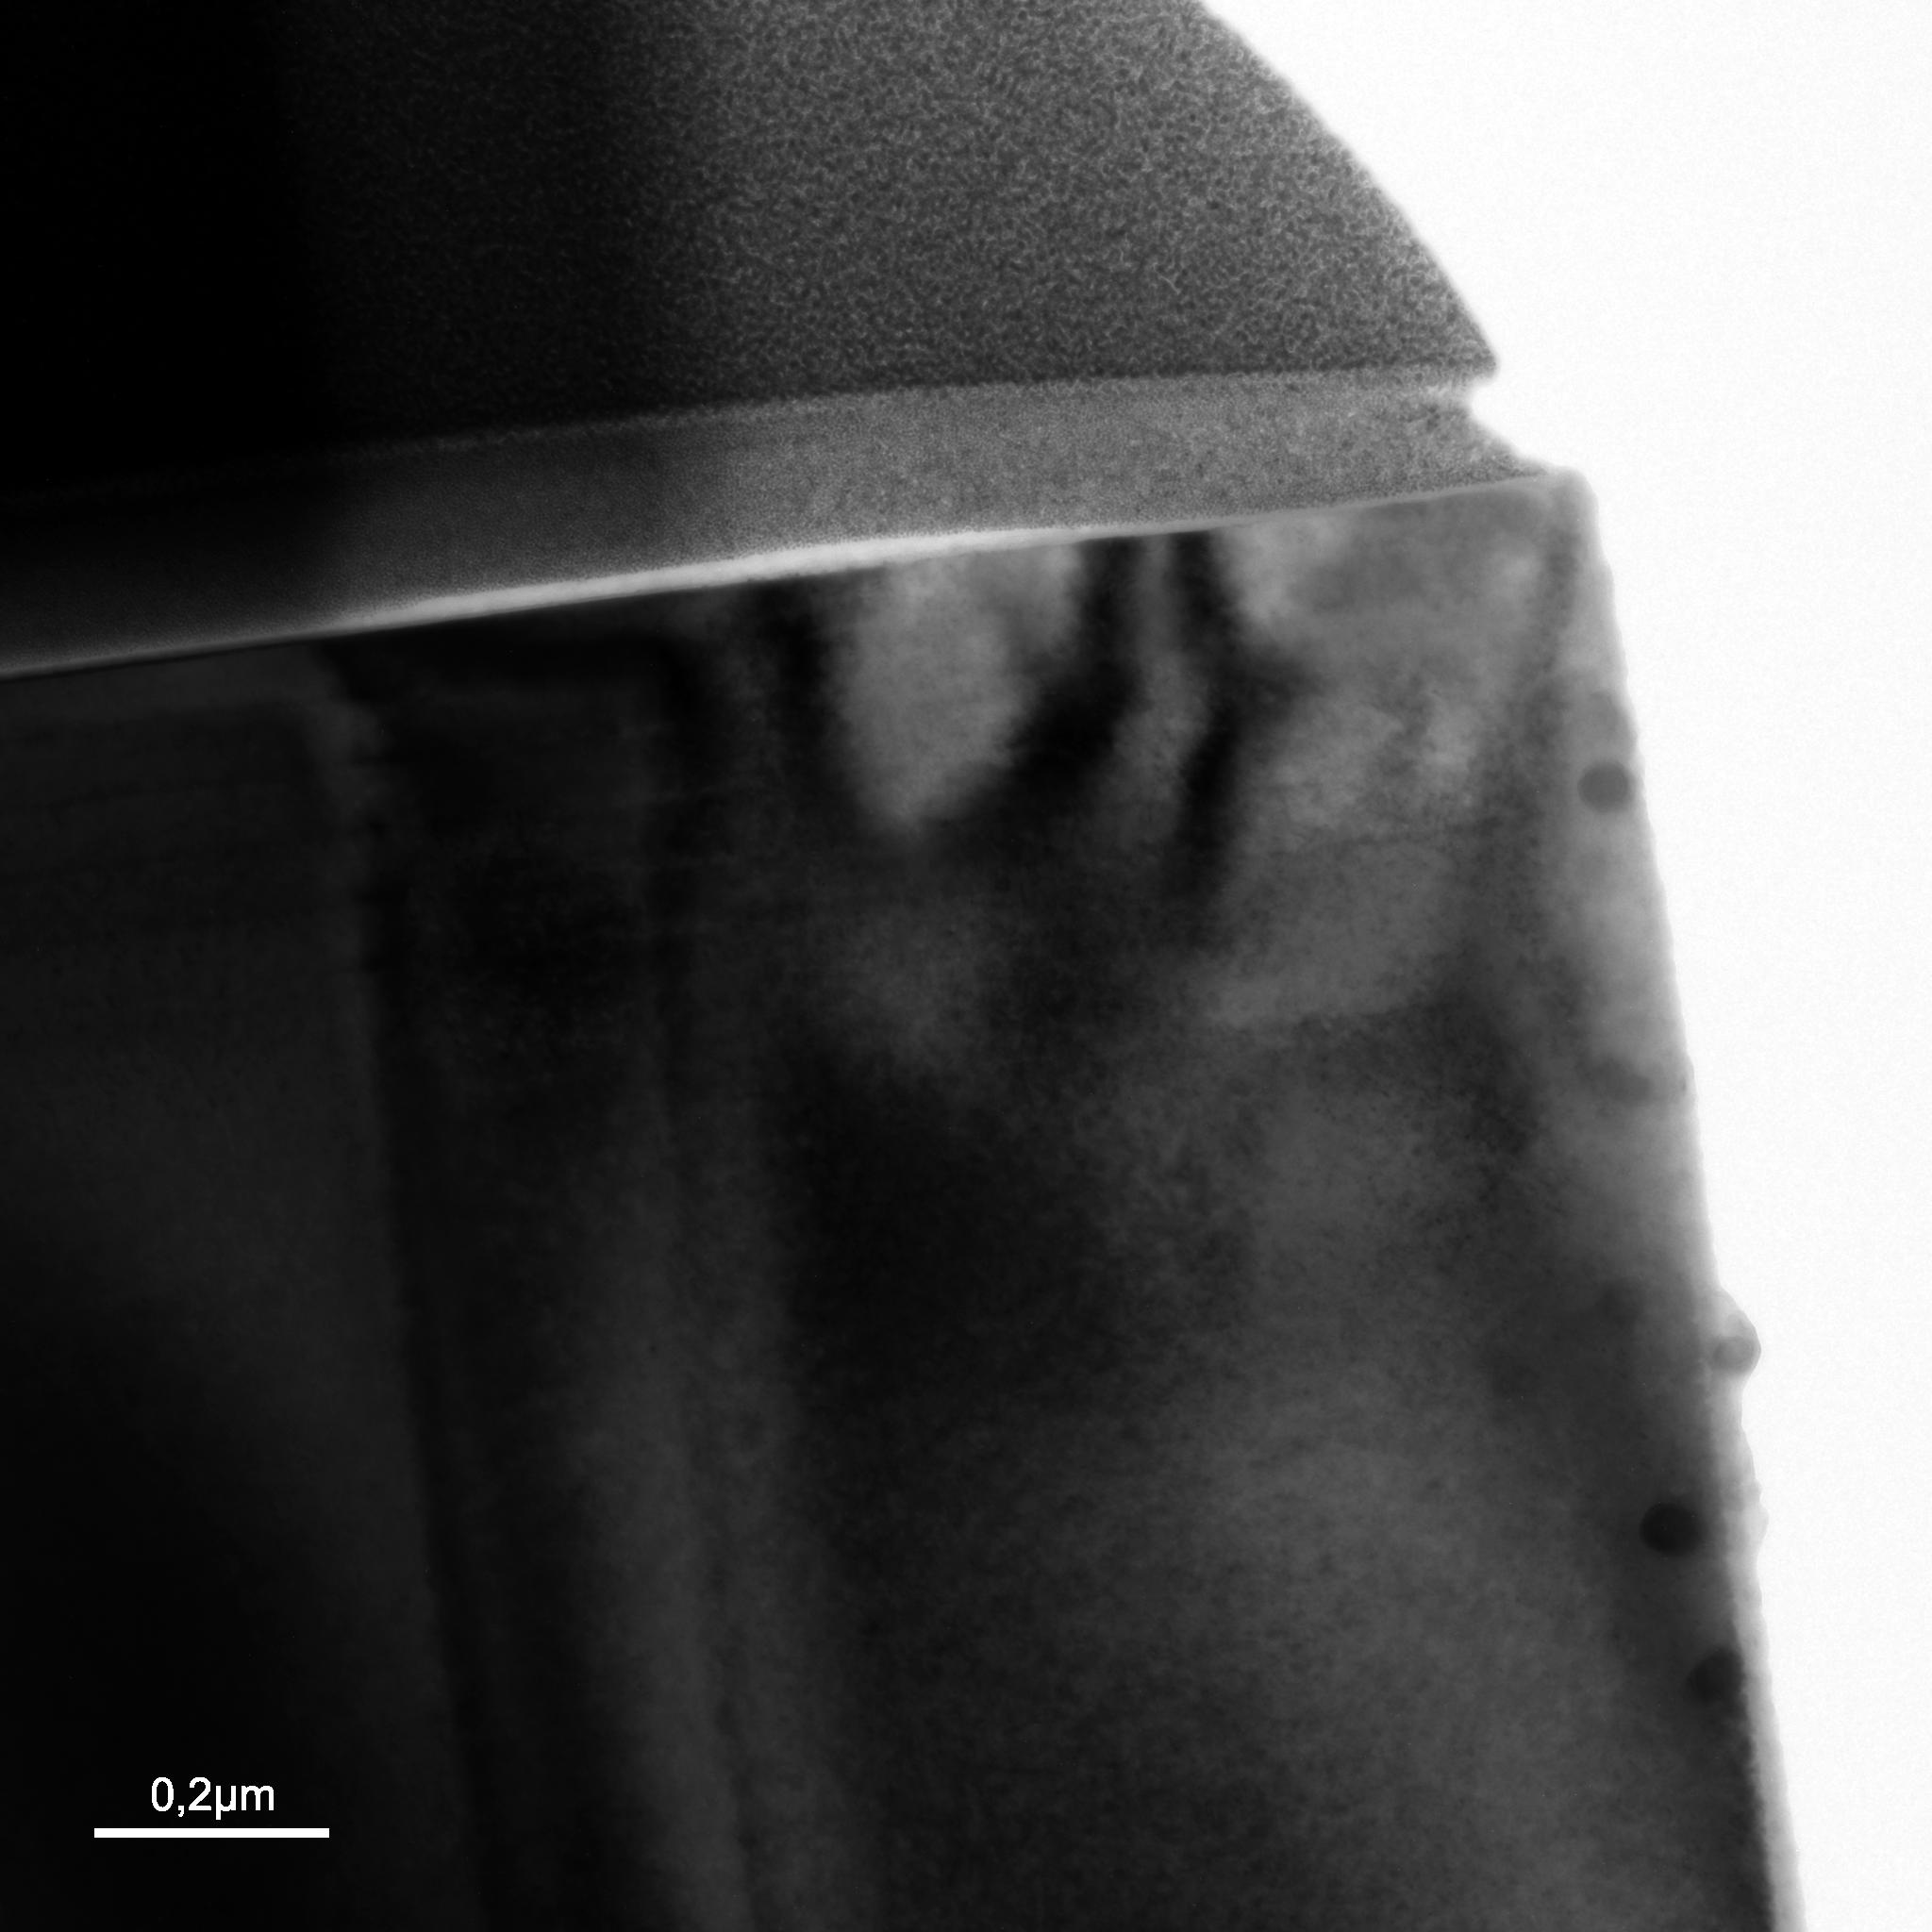
\includegraphics[width=0.32\textwidth]{Versuchsdaten/10/hell.jpg}}
	\subcaptionbox{Dunkelfeldaufnahme \\Reflex (004)\label{dunkel004}}
	[.32\linewidth]{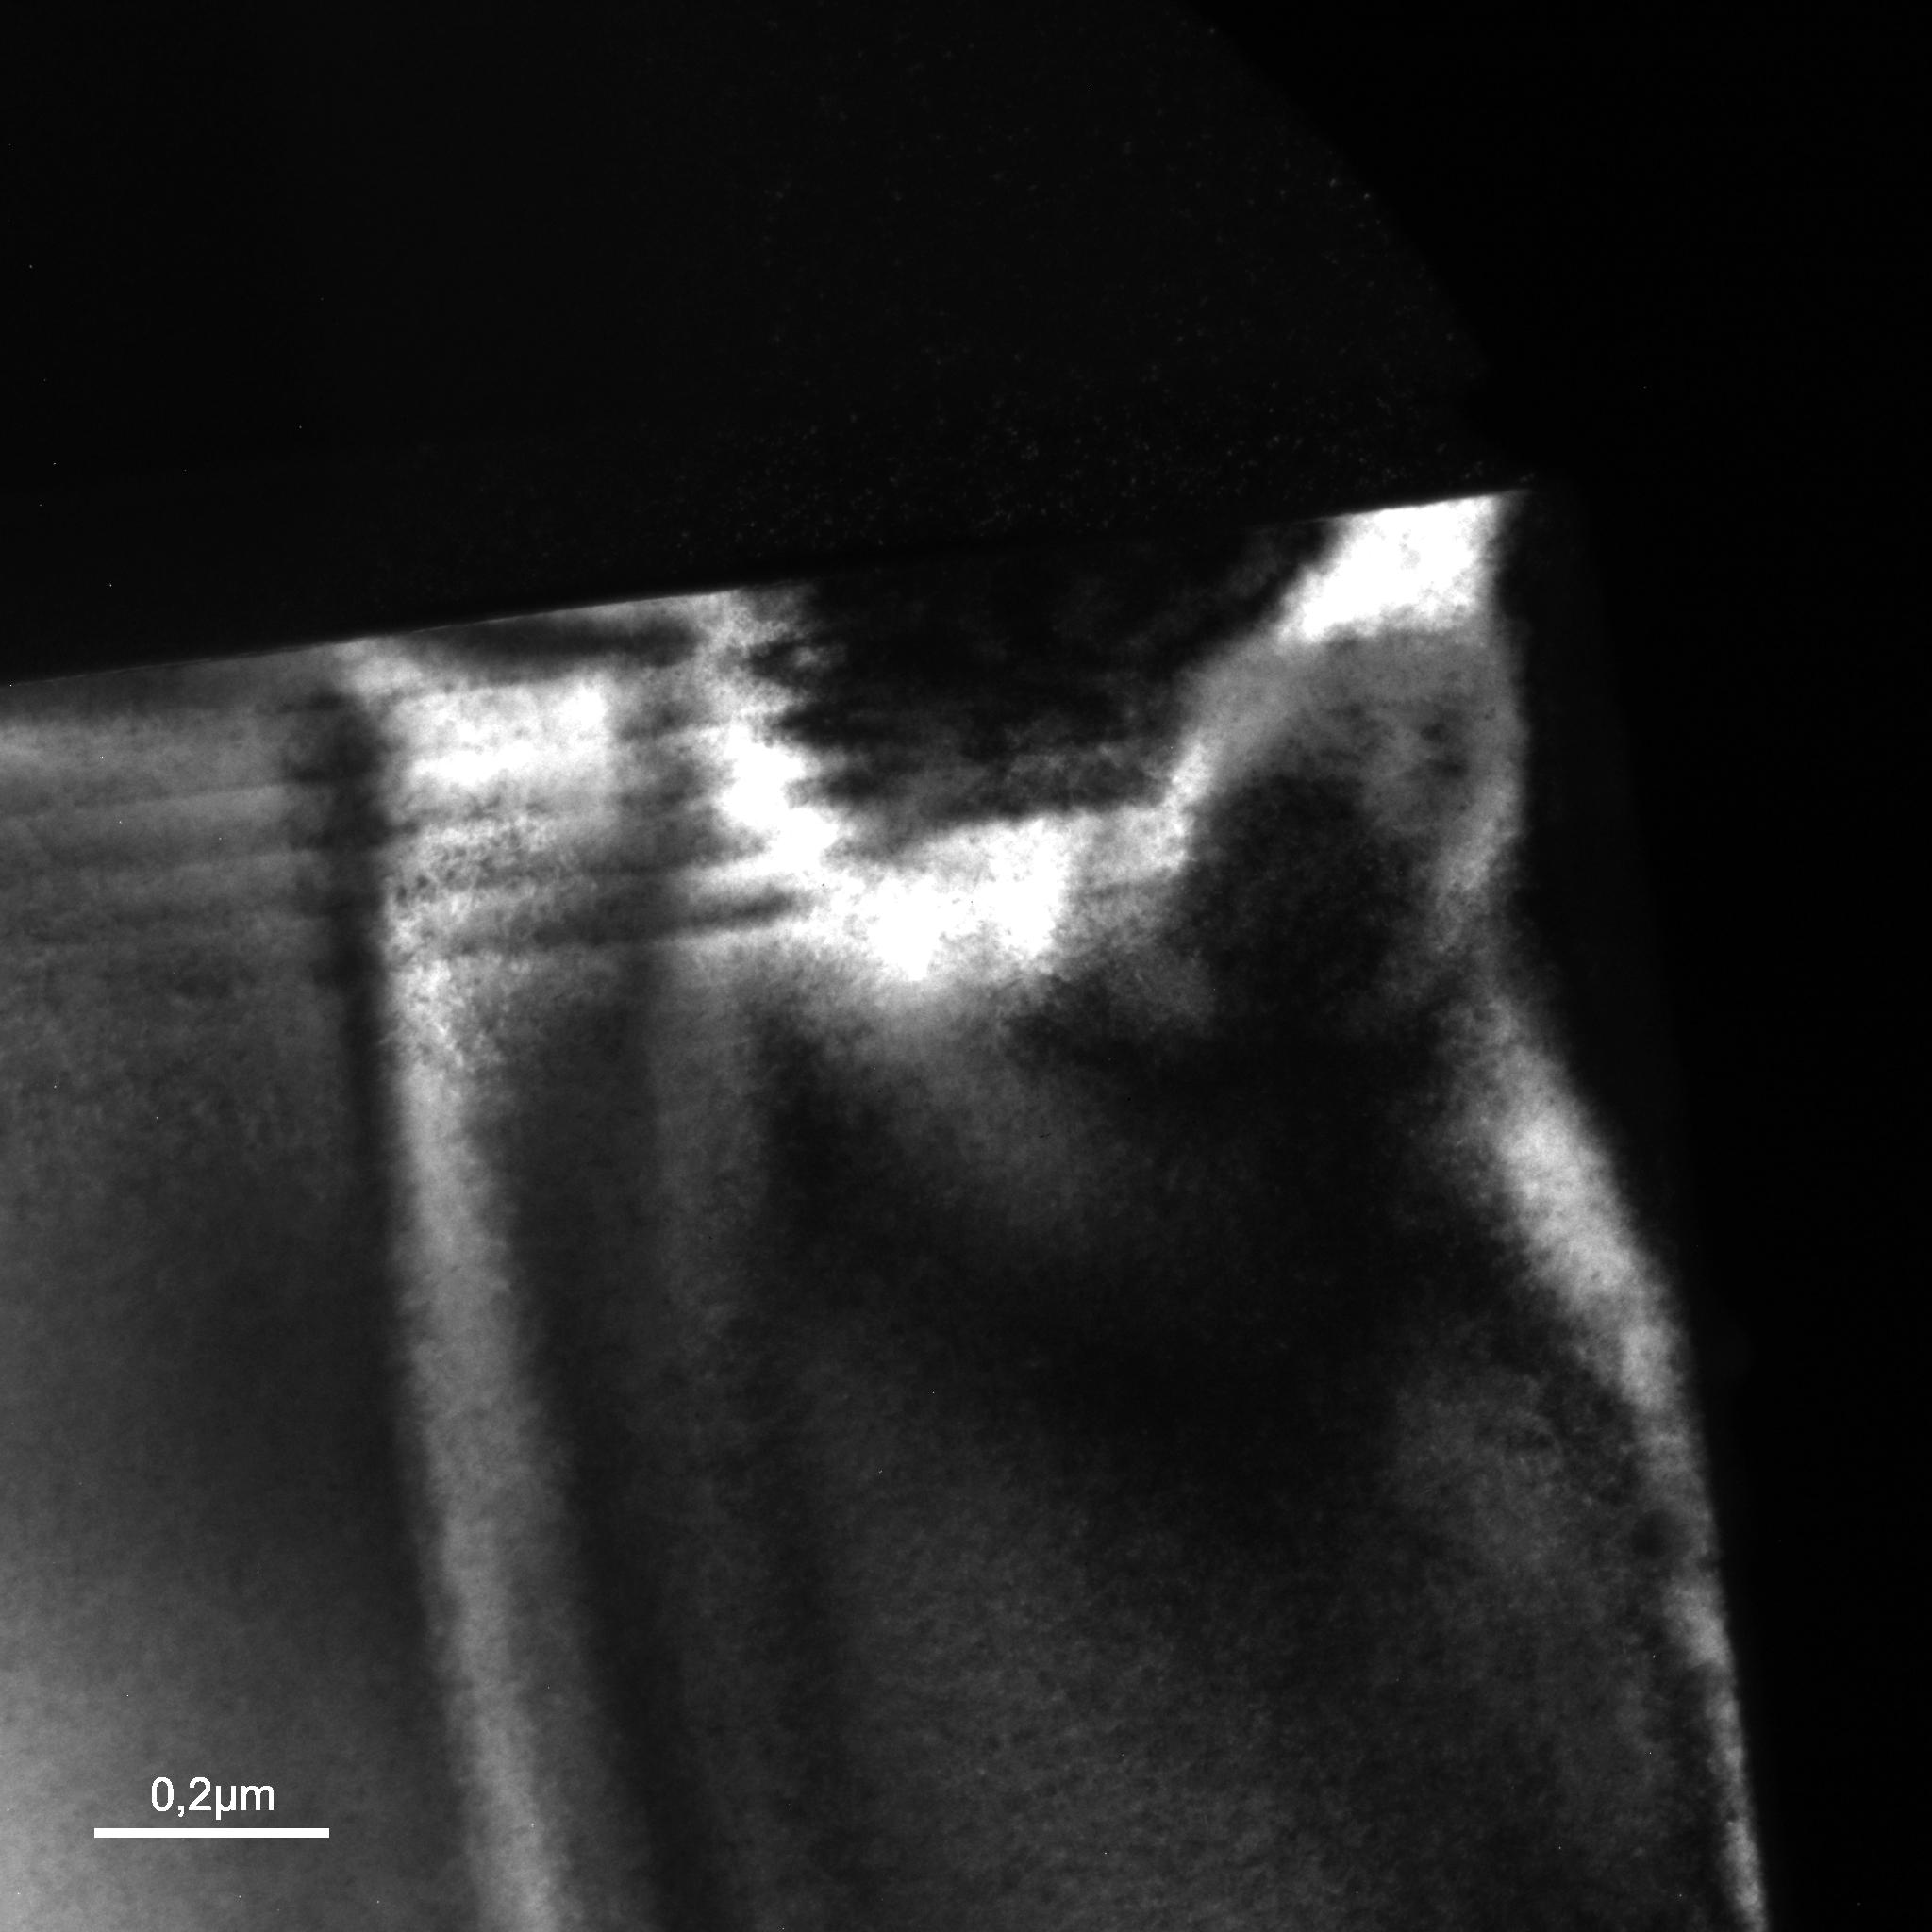
\includegraphics[width=0.32\textwidth]{Versuchsdaten/10/004-dunkel.jpg}}
	\subcaptionbox{Dunkelfeldaufnahme \\Reflex (022)\label{dunkel022}}
	[.32\linewidth]{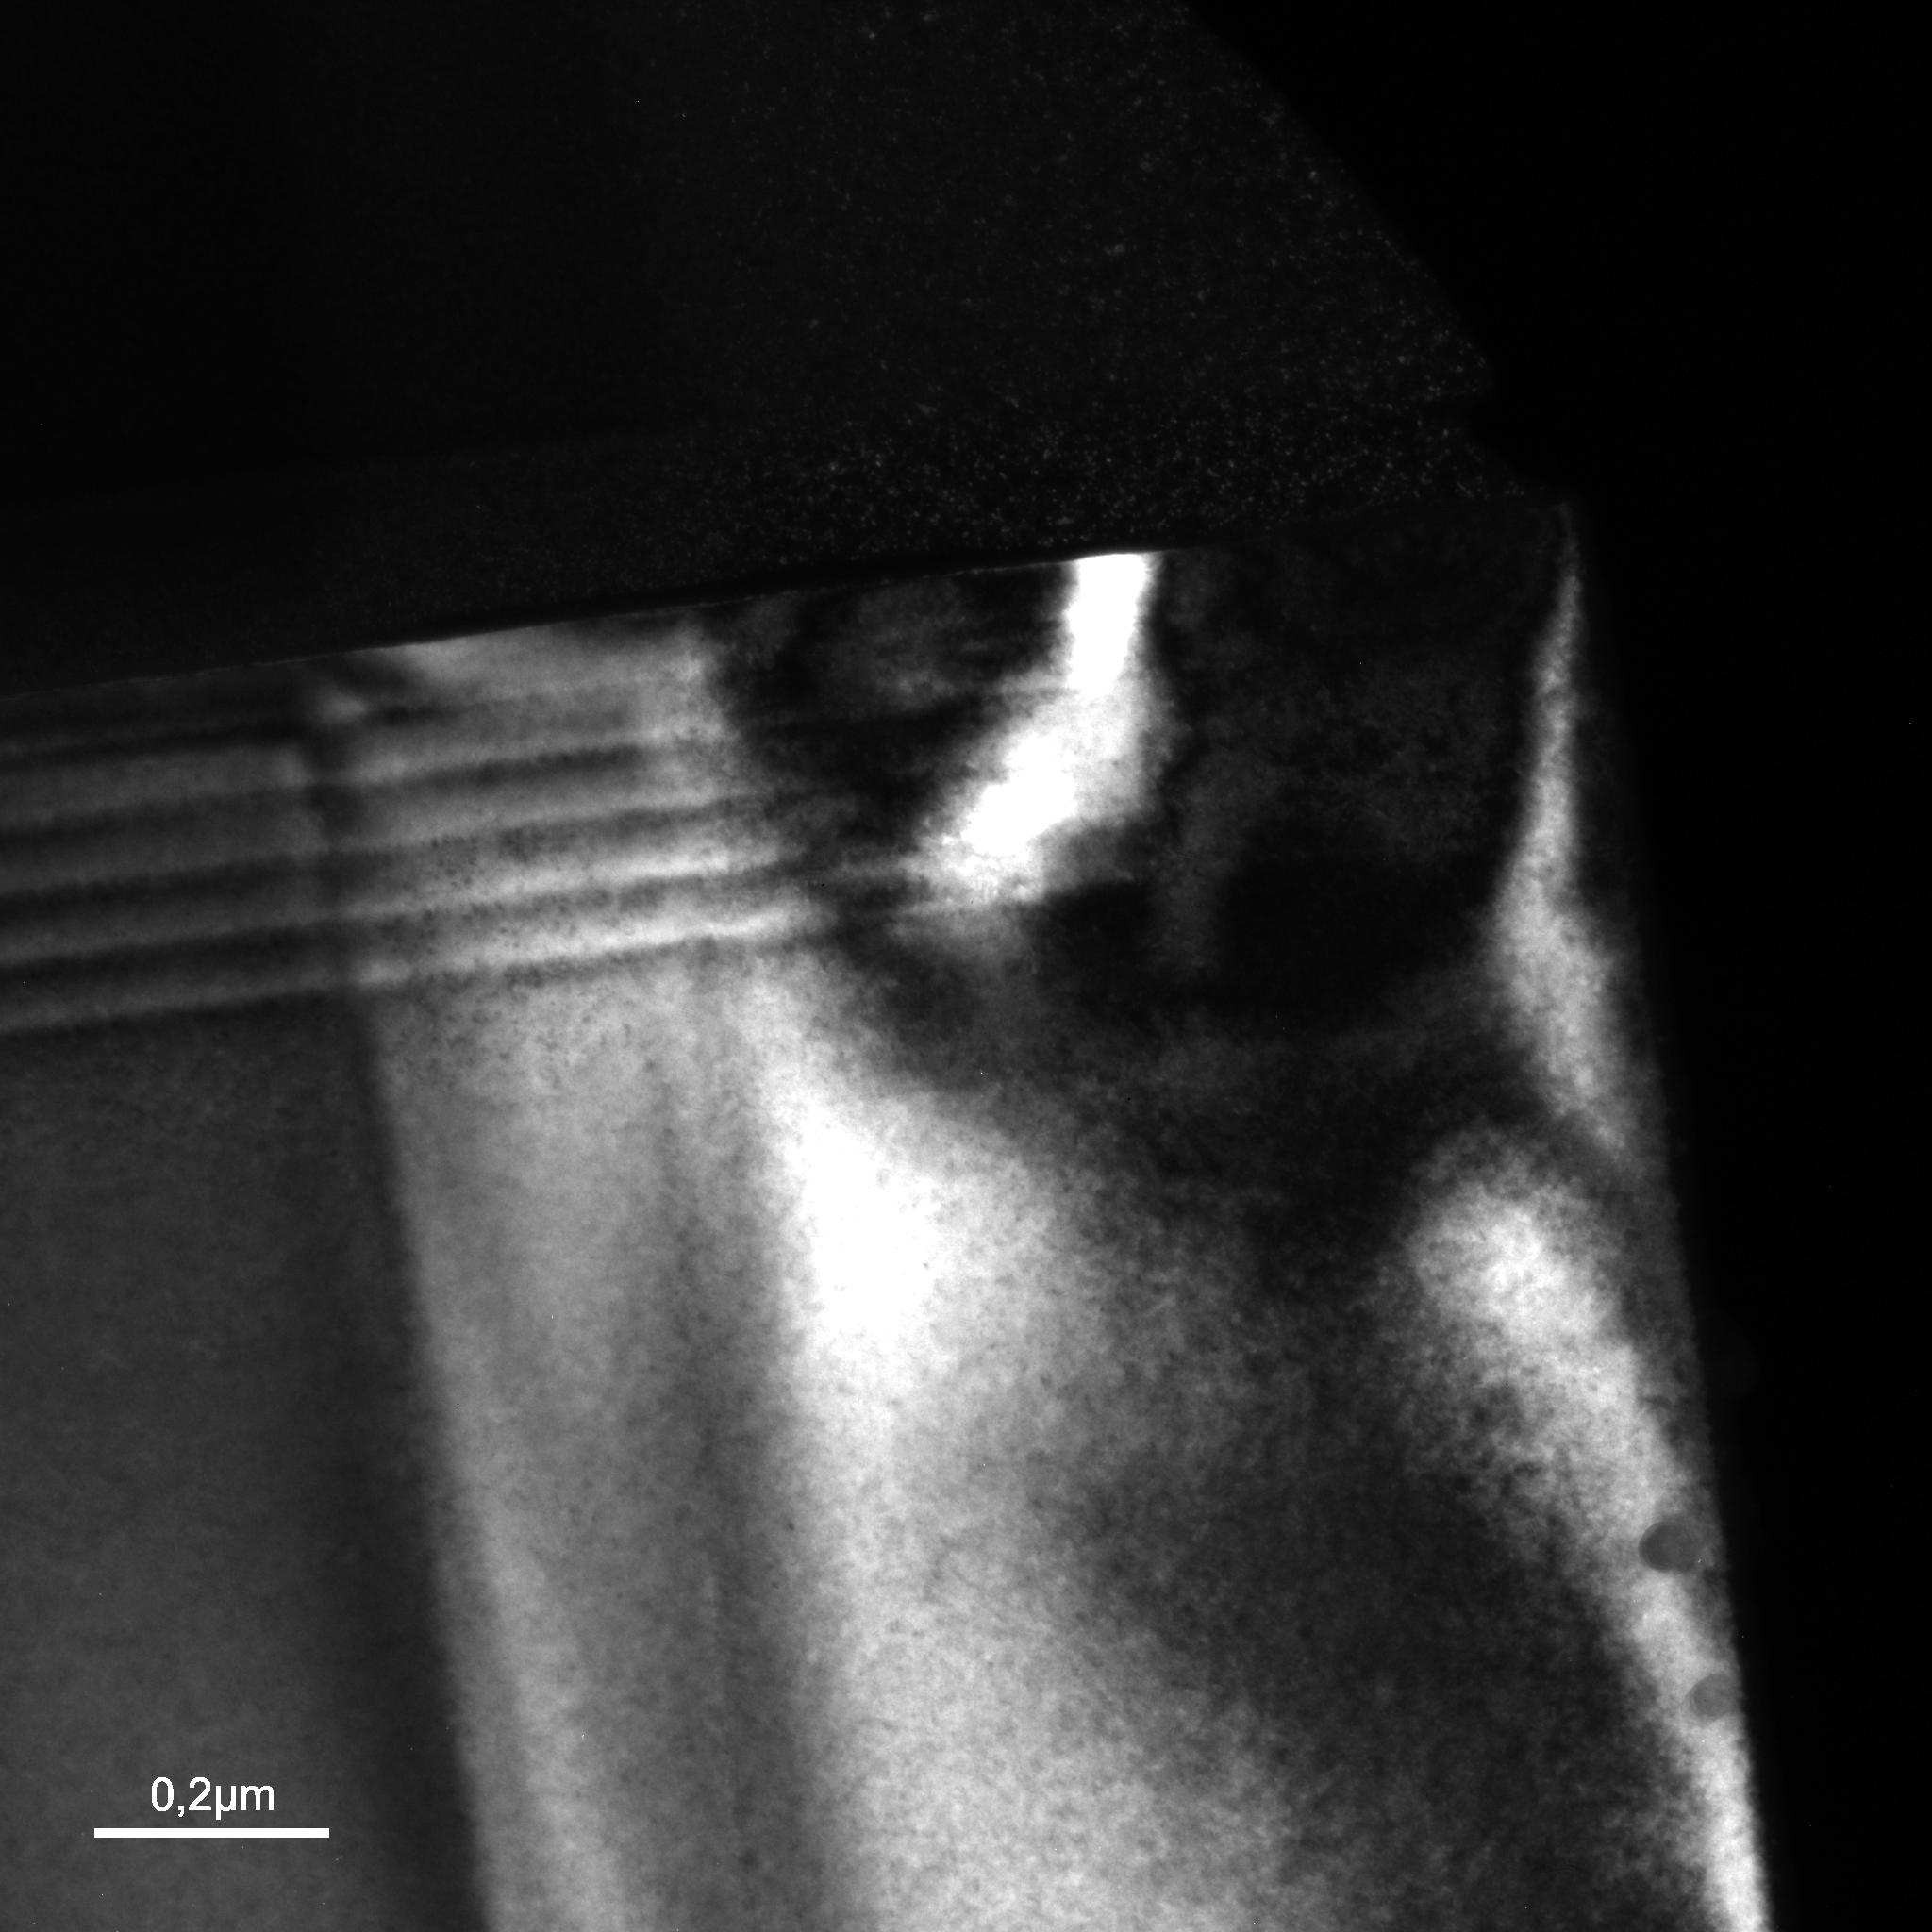
\includegraphics[width=0.32\textwidth]{Versuchsdaten/10/022-dunkel.jpg}}
	\caption{Aufnahmen der InGaAs Quantentröge} \label{dunkelhell}
\end{figure}

Zum Vergleich ist in Abb. \ref{hell} eine Hellfeldaufnahme der Probenstelle zu sehen. In den Abb. \ref{dunkel004} und \ref{dunkel022} sind zwei Dunkelfeldaufnahmen zu sehen, die mit unterschiedlichen Reflexen erstellt wurden. \\
In der Hellfeldaufnahme sind die InGaAs Quantentröge nicht sehr gut von dem umgebenen GaAs zu unterscheiden. Hierbei bieten die Dunkelfeldaufnahmen Vorteile. Da InGaAs eine andere Gitterkonstante besitzt als GaAs, sind die Reflexe nicht am gleichen Ort im Beugungsbild, sodass die InGaAs Schichten deutlich dunkler im Bild zu sehen sind. Dieser Effekt ist sowohl beim Reflex (022) als auch beim Reflex (004) zu erkennen. \\
Es sind außerdem Bereiche auf den Dunkelfeldaufnahmen zu sehen, die ebenfalls dunkel erscheinen und keine Einzelheiten mehr erkennen lassen. Dies könnten Bereiche sein, in denen die Probe eine unterschiedliche Kristallorientierung besitzen und dadurch der jeweilige Reflex verschoben oder schwächer ausgeprägt ist. \\
In Abb. \ref{trogdunkel} im Anhang sind (020) Dunkelfeldaufnahmen der InGaAs-Quantentröge zu sehen. Da die InGaAs-Schichten den Reflex (020) nicht am gleichen Ort, wie GaAs besitzt, erscheinen die Quantentröge mit einer sehr viel schwächeren Intensität, sodass sie schwarz aussehen.
In Abb. \ref{trogdunkel} im Anhang sind (020) Dunkelfeldaufnahmen der InGaAs-Quantentröge zu sehen. Da die InGaAs-Schichten den Reflex (020) nicht am gleichen Ort, wie GaAs besitzt, erscheinen die Quantentröge mit einer sehr viel schwächeren Intensität, sodass sie schwarz aussehen.


\begin{figure}[htb]\centering
	\subcaptionbox{34000-fache Vergrößerung\label{34kaus}}
	[.49\linewidth]{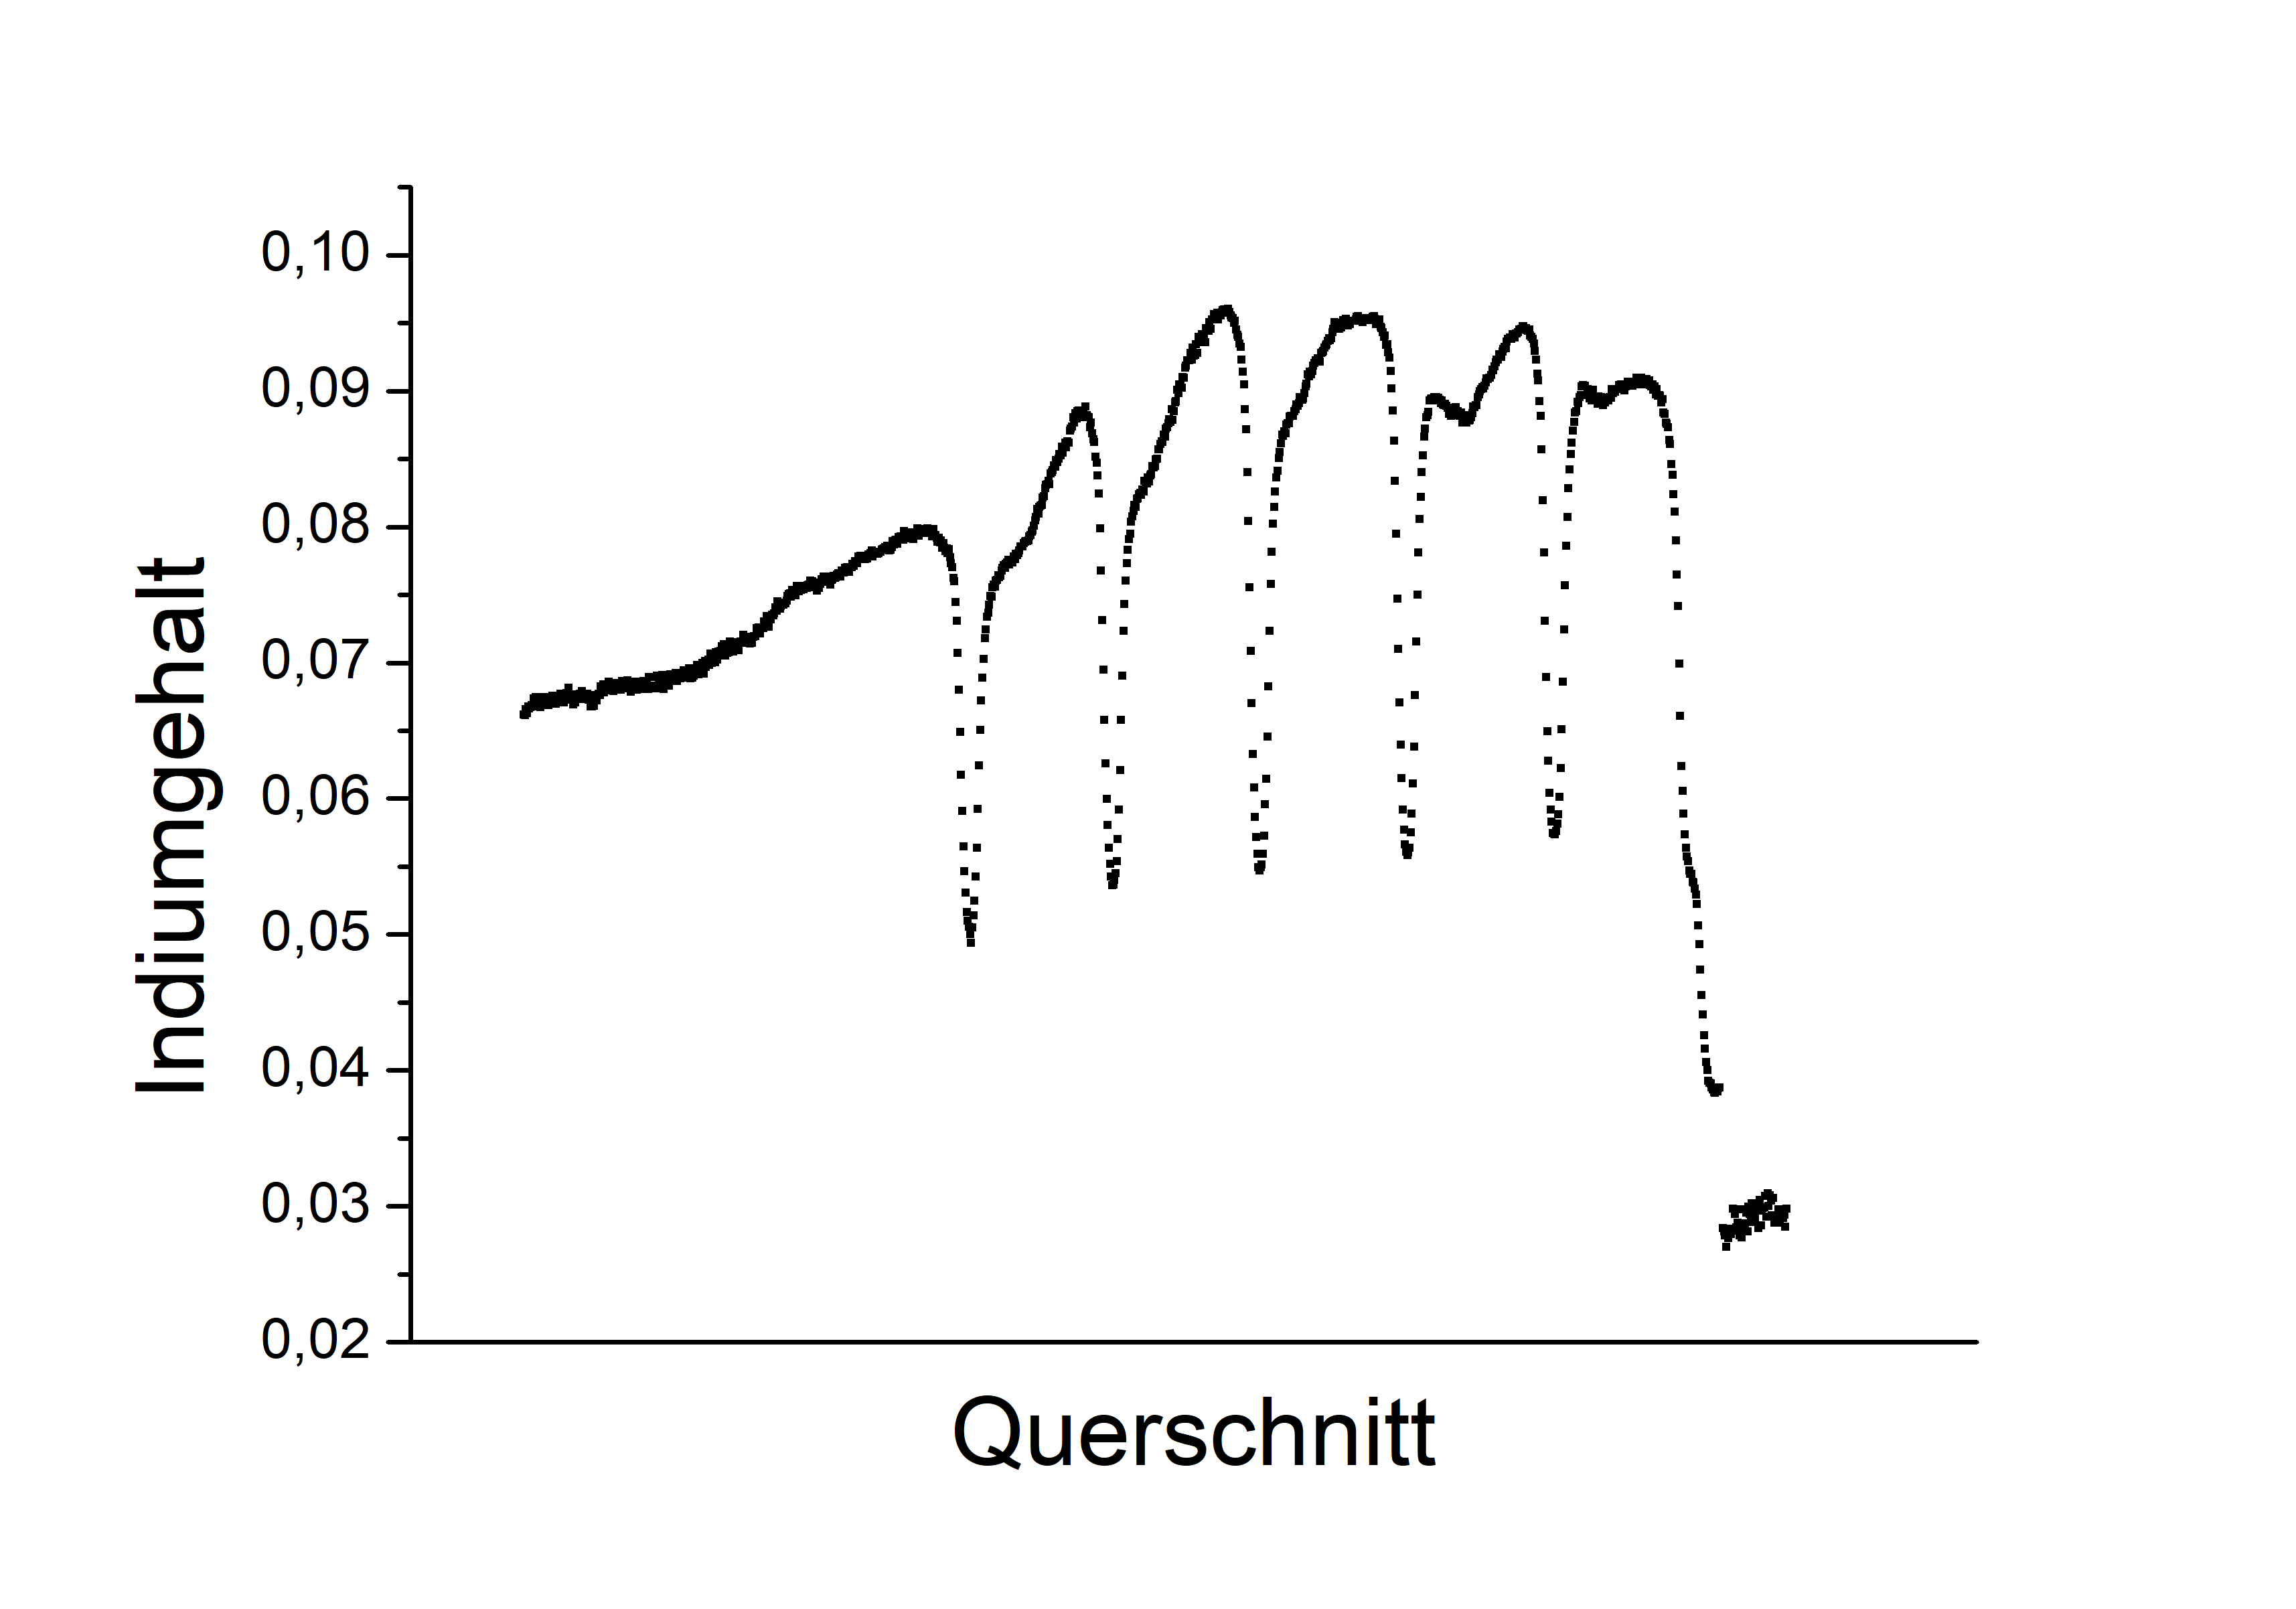
\includegraphics[width=0.49\textwidth]{Versuchsdaten/11/34000xausschnitt.png}}
	\subcaptionbox{87000-fache Vergrößerung\label{87kaus}}
	[.49\linewidth]{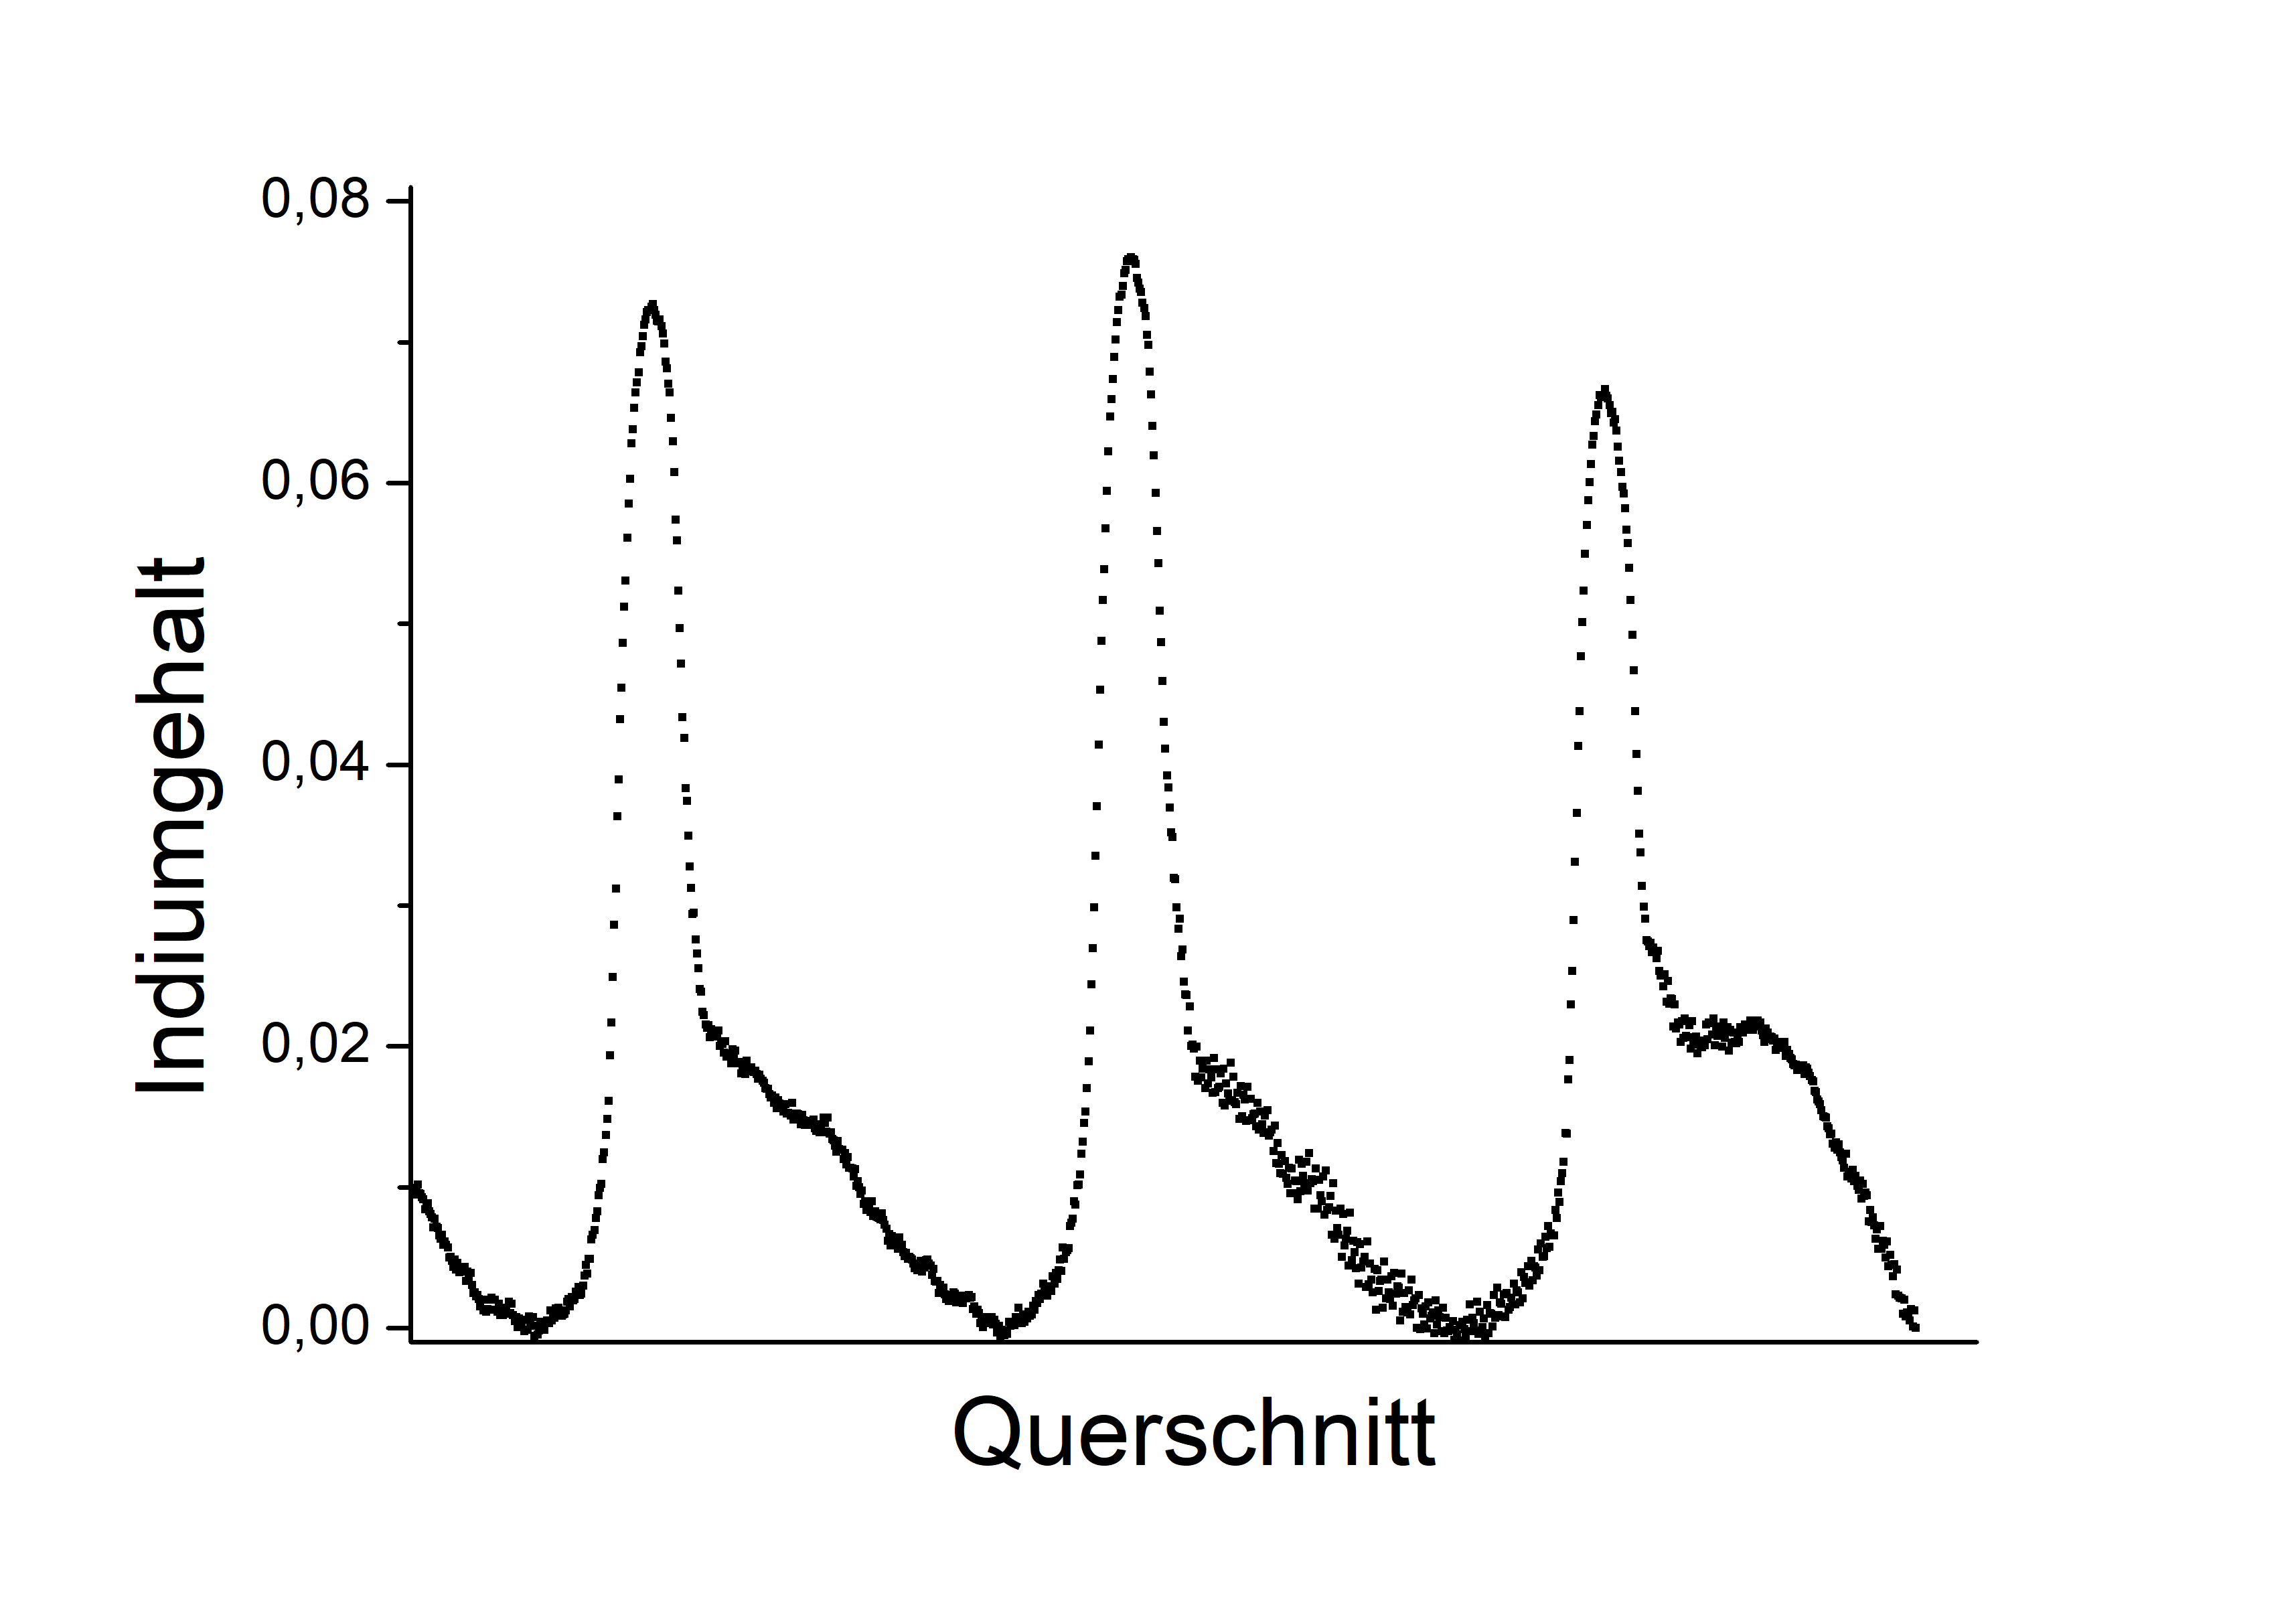
\includegraphics[width=0.49\textwidth]{Versuchsdaten/11/87000xausschnitt.png}}\\
	\subcaptionbox{185000-fache Vergrößerung\label{185kaus}}
	[.49\linewidth]{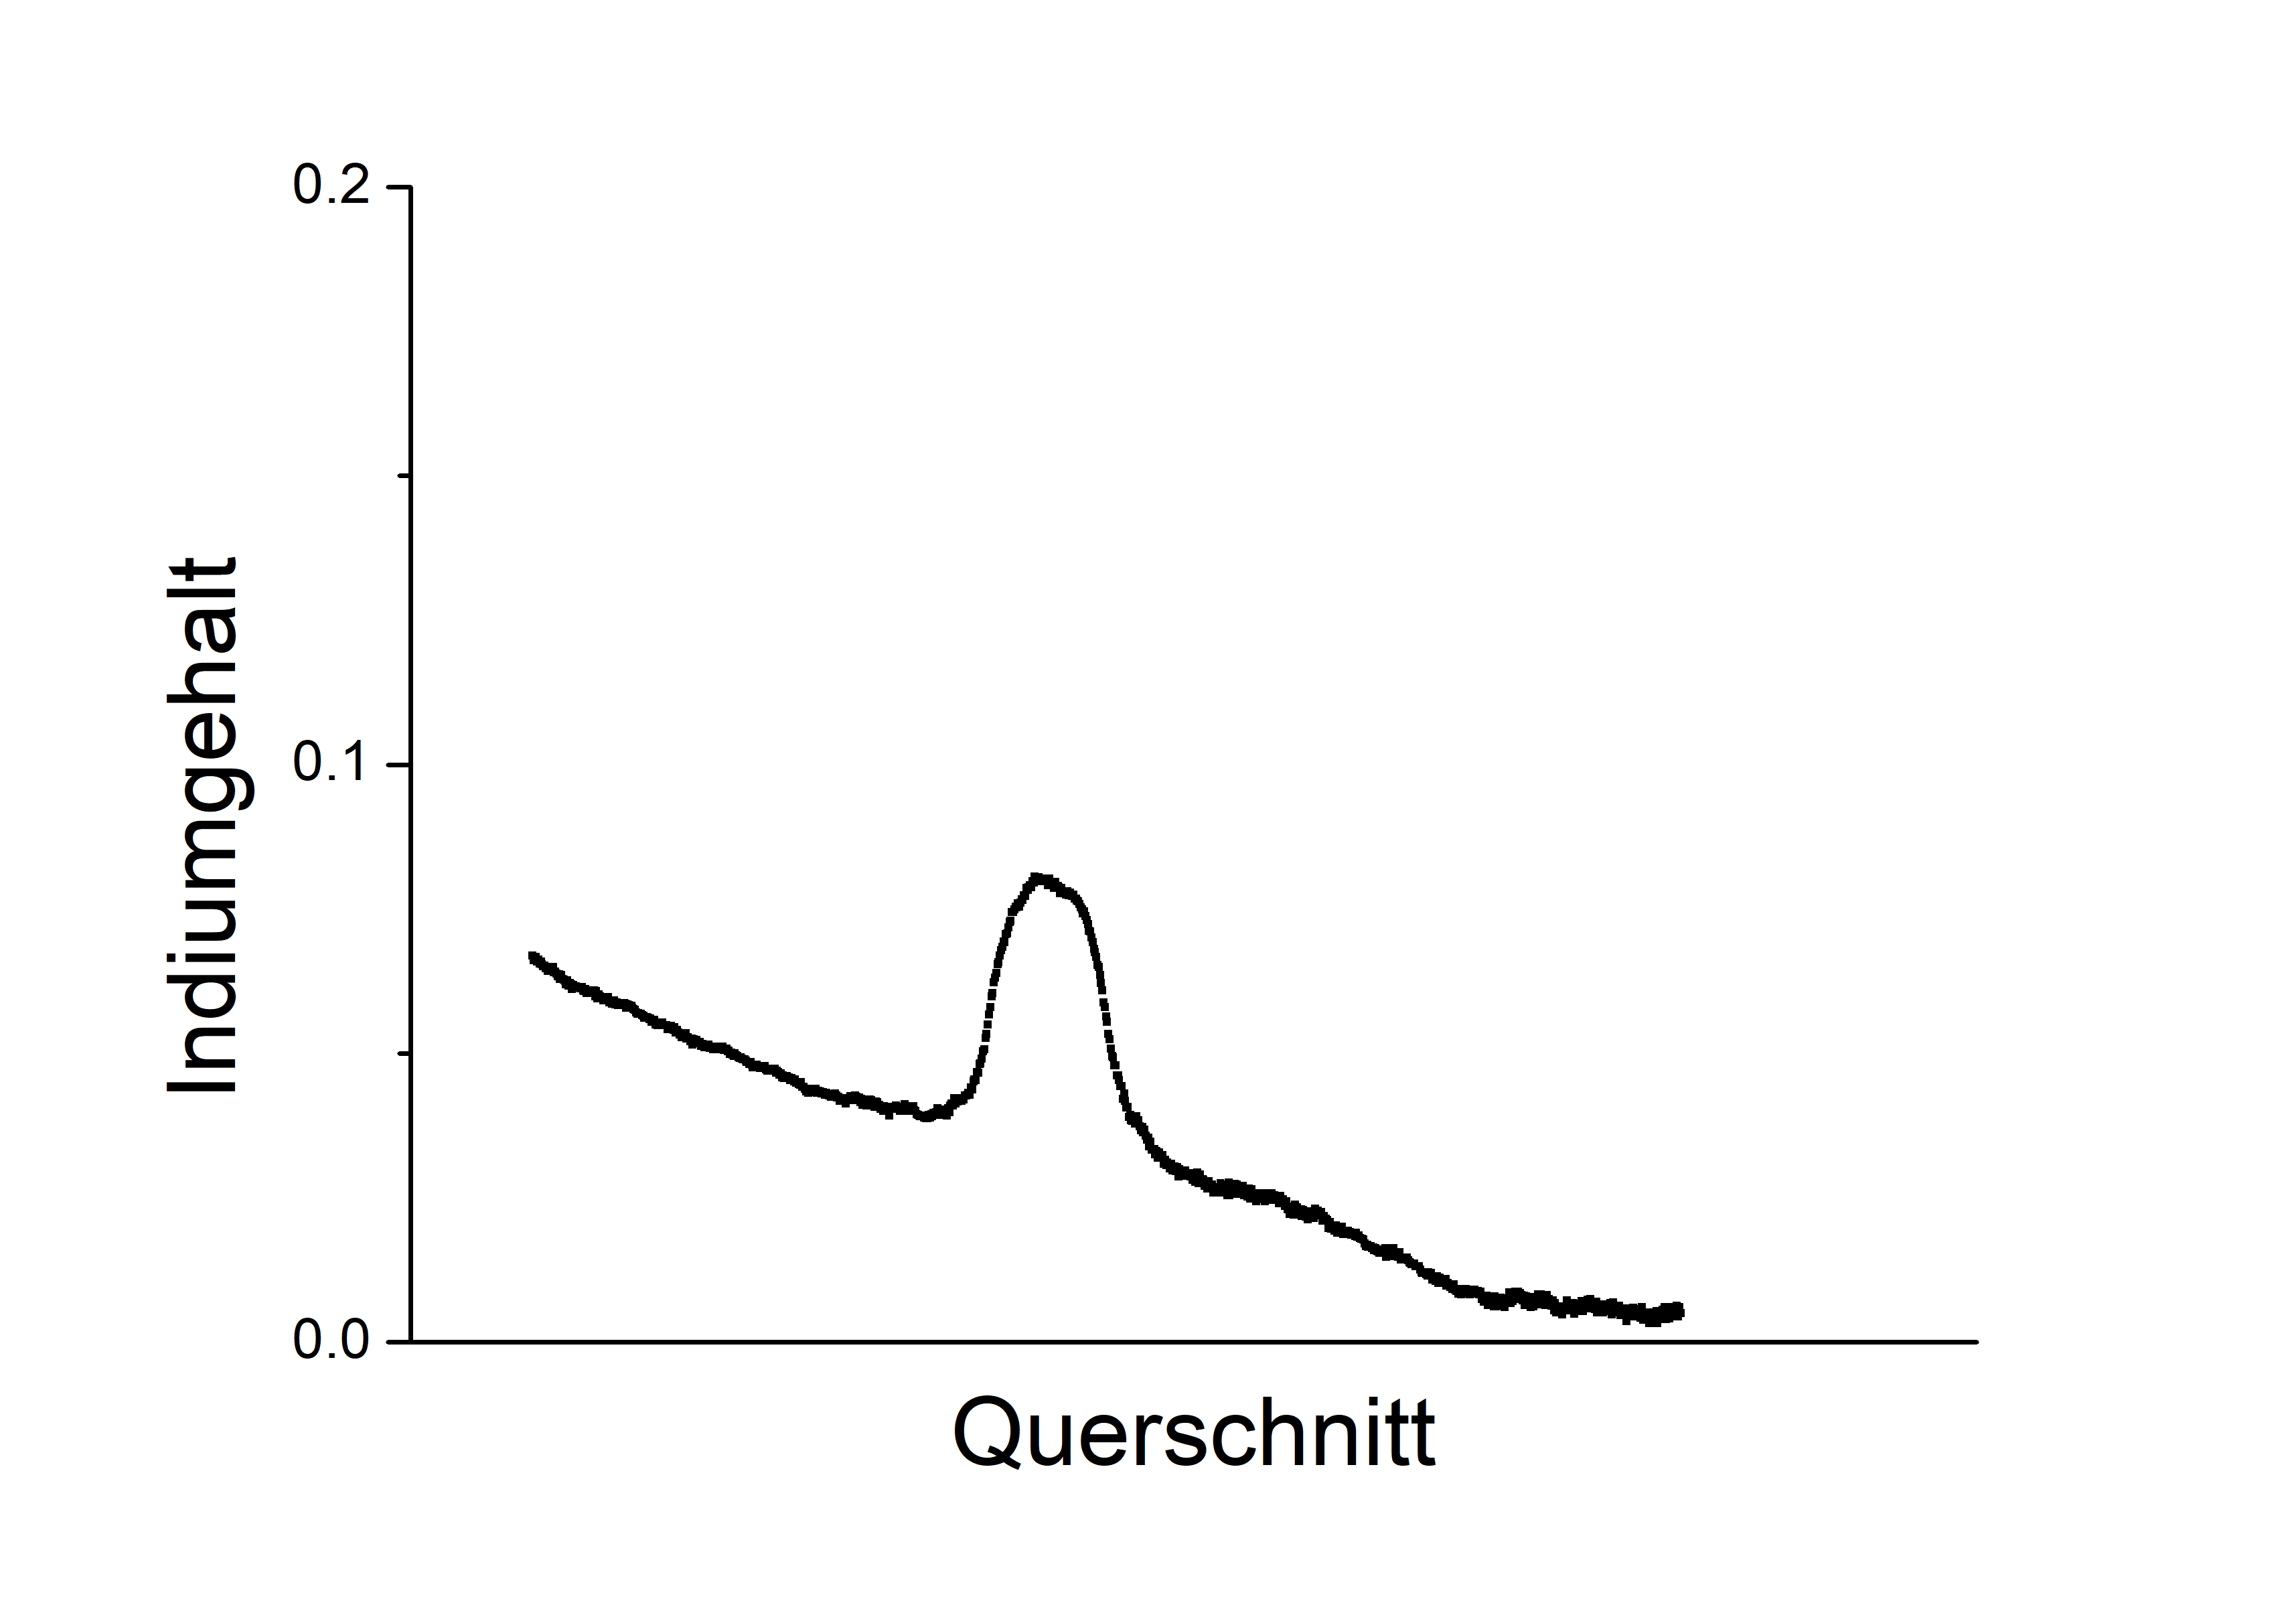
\includegraphics[width=0.49\textwidth]{Versuchsdaten/11/185000xausschnitt.png}}
	\subcaptionbox{380000-fache Vergrößerung\label{380kaus}}
	[.49\linewidth]{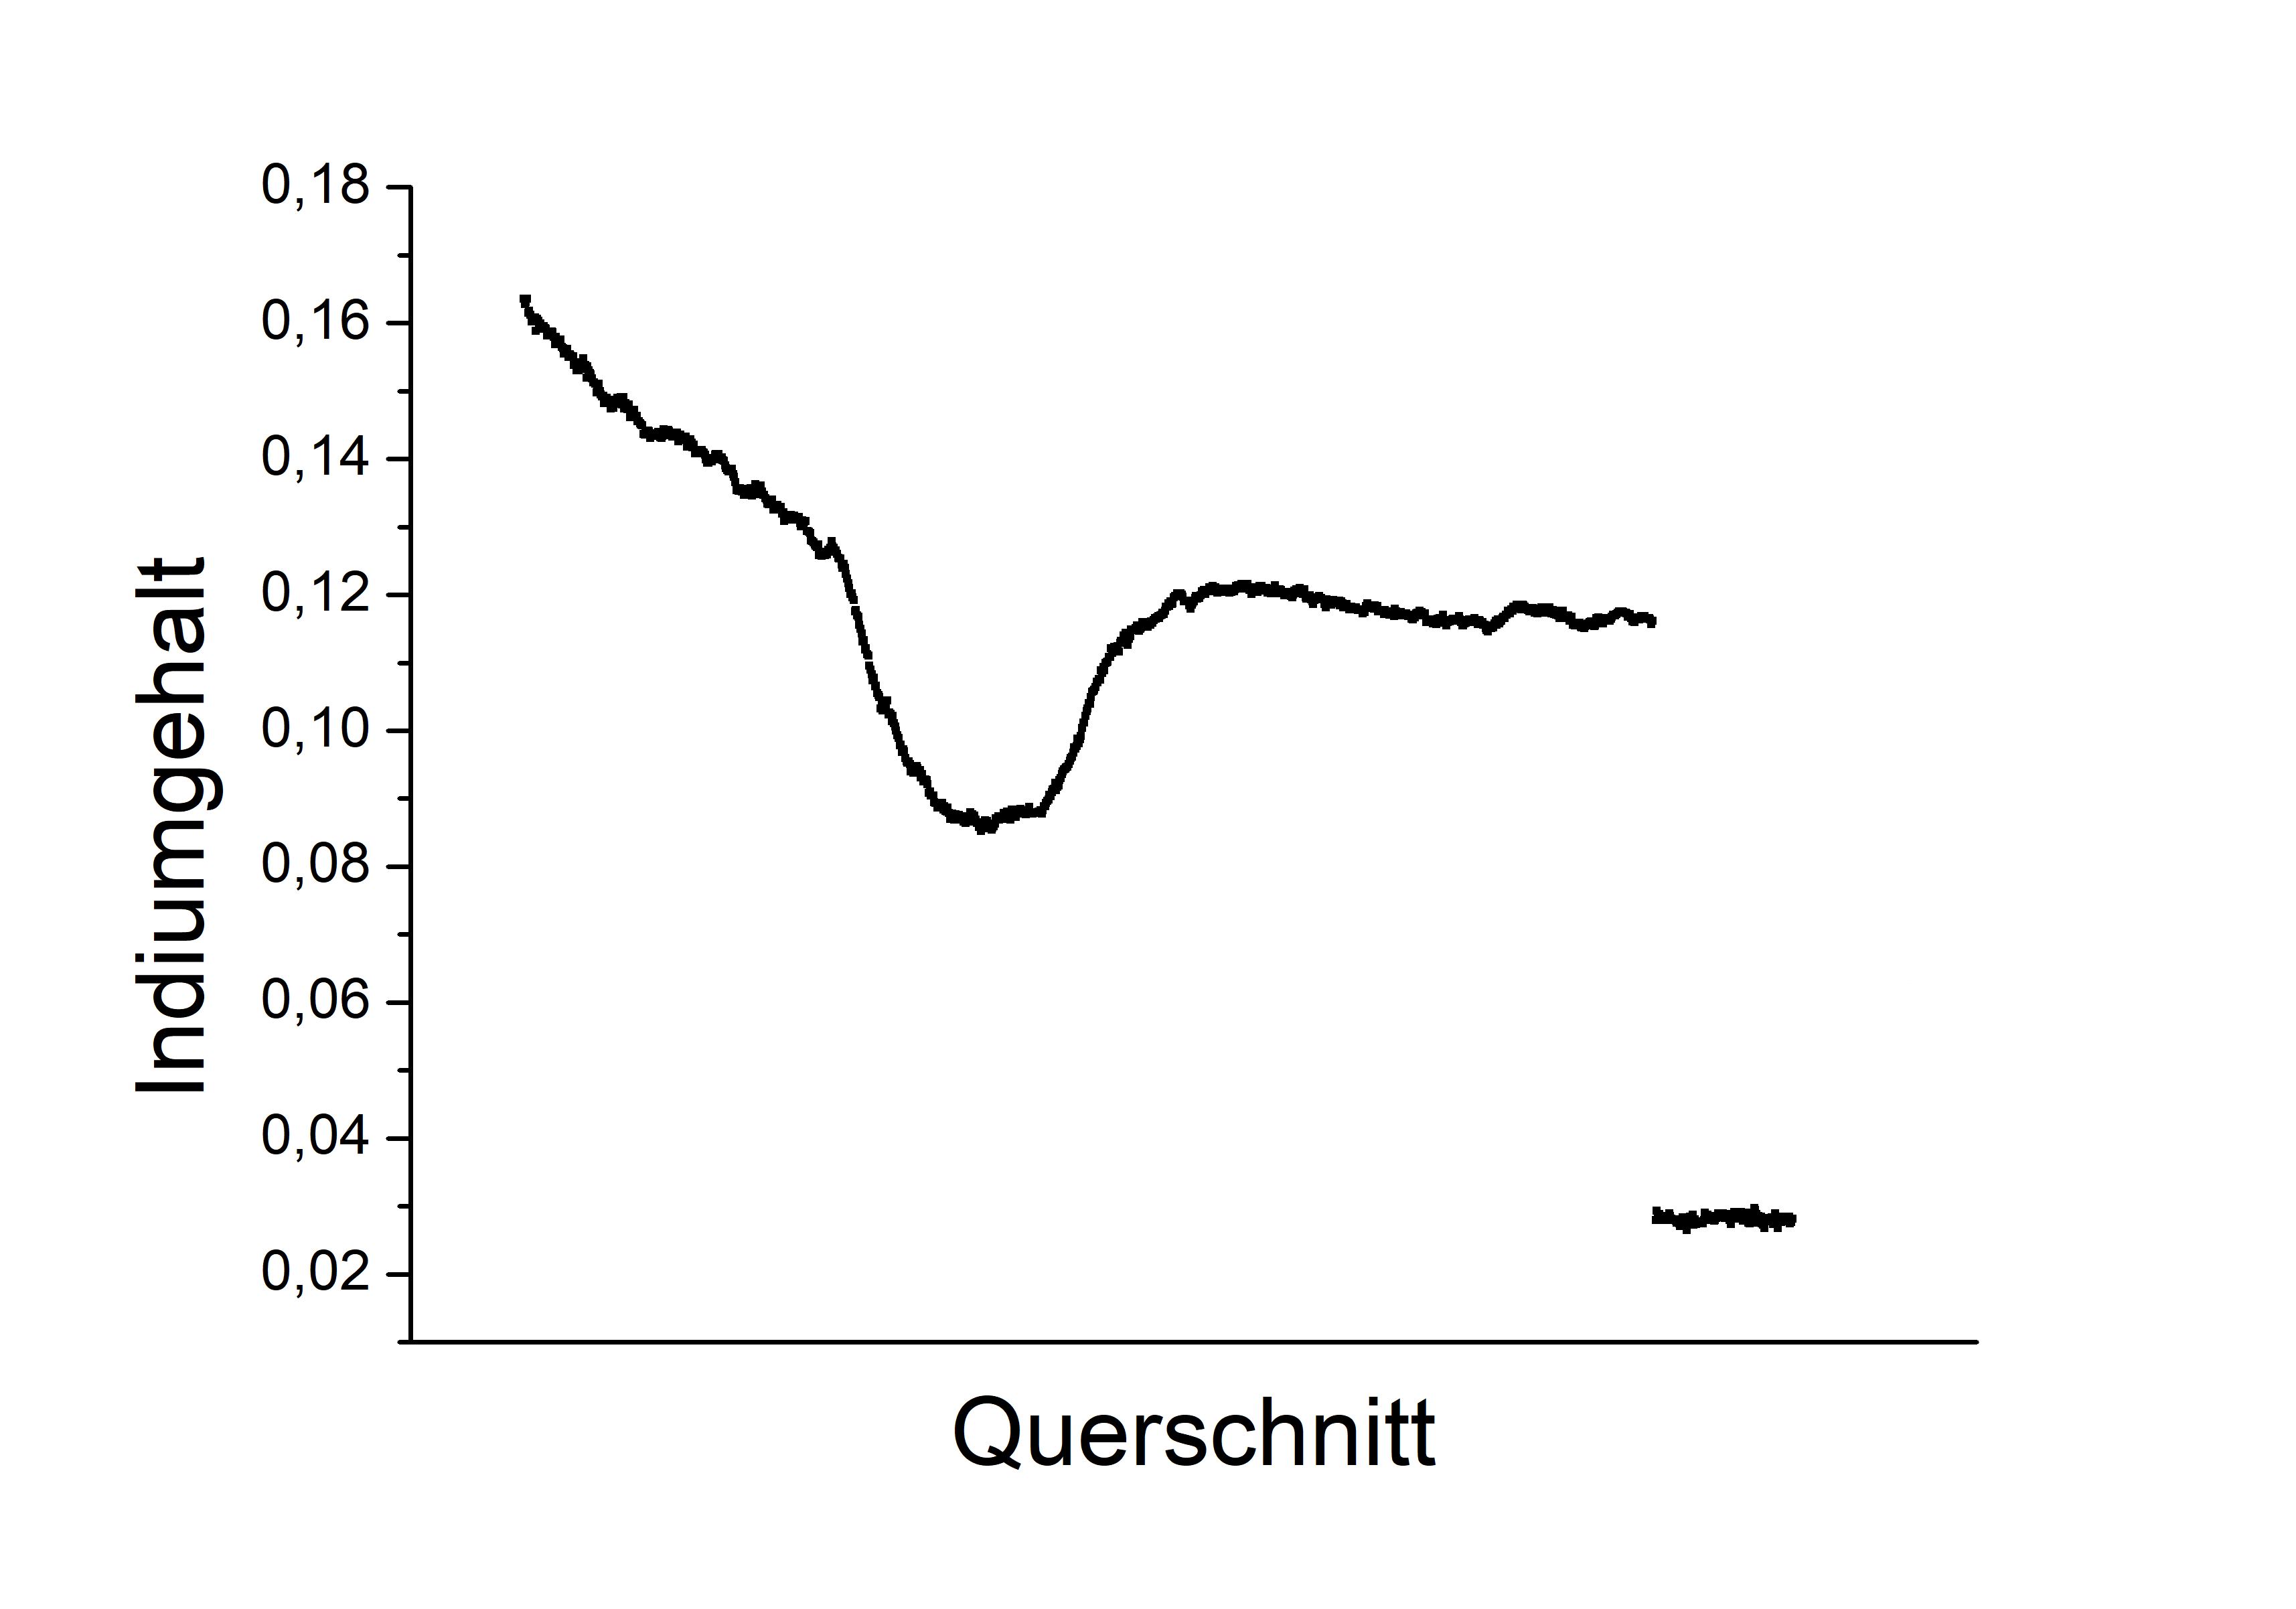
\includegraphics[width=0.49\textwidth]{Versuchsdaten/11/380000xausschnitt.png}}

	\caption{Indiumgehalt der Ausschnitte im Querschnitt} \label{indprofil}
\end{figure}

Aus den Aufnahmen in Abb. \ref{trogdunkel} sind Intensitätsprofile über den Querschnitt senkrecht zu den Quantentrögen erstellt worden. Da die Intensität vom Indiumgehalt abhängt, konnte der Indiumgehalt über dem Querschnitt dargestellt werden. Die Ergebnisse sind in Abb. \ref{indprofil} dargestellt. \\
Außerhalb der Quantentröge wurde hierfür der Indium Gehalt innerhalb der GaAs-Schichten als 0 angenommen. Auf diesen Intensitätswert wurde der Rest des Intensitätprofils normiert. Da die Intensität quadratisch vom (020) Strukturfaktor abhängt, konnte aus dem Strukturfaktor $F(x)$ der Indiumgehalt $x$ in Abhängigkeit von der Intensität $I$ bestimmt werden. Aus der gegebenen Abhängigkeit wurde abgelesen:
\begin{align*}
	I \sim F^2 \\
	\dfrac{I(x)}{I(0)} = \left\vert\dfrac{F(x)}{F(0)}\right\vert^2
\end{align*}

Diese Beziehung wird nach $F(x)$ umgestellt und dann nach $x$ aufgelöst. Hierzu wurde die Abhängikeit des Strukturfaktors im (020) Reflex vom Indiumgehalt $F(x) = (0,95x - 0,15)\,\mathrm{nm}$ genutzt.

\begin{align*}
	F(x) = \pm\sqrt{\dfrac{I(x)}{I(0)}}\vert F(0) \vert \\
	x = \dfrac{\pm\sqrt{\dfrac{I(x)}{I(0)}}\vert F(0)\vert - F(0)}{0,95}
\end{align*}

Wobei $F(0) = -0,15\,\mathrm{nm}$ ist. Die positive Wurzel würde dabei für Konzentrationen größer als $\frac{0,15}{0,95}$ stehen, weshalb hier die negative Lösung genutzt wird. \\
Mit dieser Gleichung konnten die normierten Intensitätsprofile zu Indiumgehaltsprofilen umgerechnet werden. Die Quadratfunktion hat zwei Lösungen, von der die Negative verwendet werden muss, damit bei einer normierten Intensität von 1 der Indiumgehalt 0 wird. \\
Zuletzt wurde der Indiumgehalt zusätzlich mithilfe eines Hochauflösungs-TEM Bildes bestimmt. Hierbei wurde keine Dunkelfeldaufnahme verwendet, um die Intensitäten zu bestimmen, sondern stattdessen die Gitterkonstanten aus den Atomabständen bestimmt. Aus der Abhängigkeit der Gitterkonstante $a$ vom Indiumgehalt, konnte der Indiumgehalt von der Gitterkonstante abhängig gemacht werden. \\
Das Hochauflösungs-TEM Bild ist in Abb. \ref{hochtem} im Anhang zu sehen. Da im Versuch selbst kein verwendbares Hochauflösungsbild erstellt werden konnte, wurde ein passendes Ergebnis aus älteren Versuchen zur Verfügung gestellt. In Abb. \ref{filthoch} im Anhang wurden mit der Software Image eval die Netzebenenabstände vermessen und daraus ein Profil der Gitterverzerrung durch den Quantentrog erstellt. \\
Mit der gegebenen Abhängigkeit zwischen Gitterkonstante und Indiumgehalt konnte daraus mit folgender Umrechnung ein Profil des Indiumgehalts erstellt werden, welches in Abb. \ref{hochindium} dargestellt ist:

\begin{align*}
	(x-1) / 0.0718
\end{align*}

\begin{figure}[H]\centering
	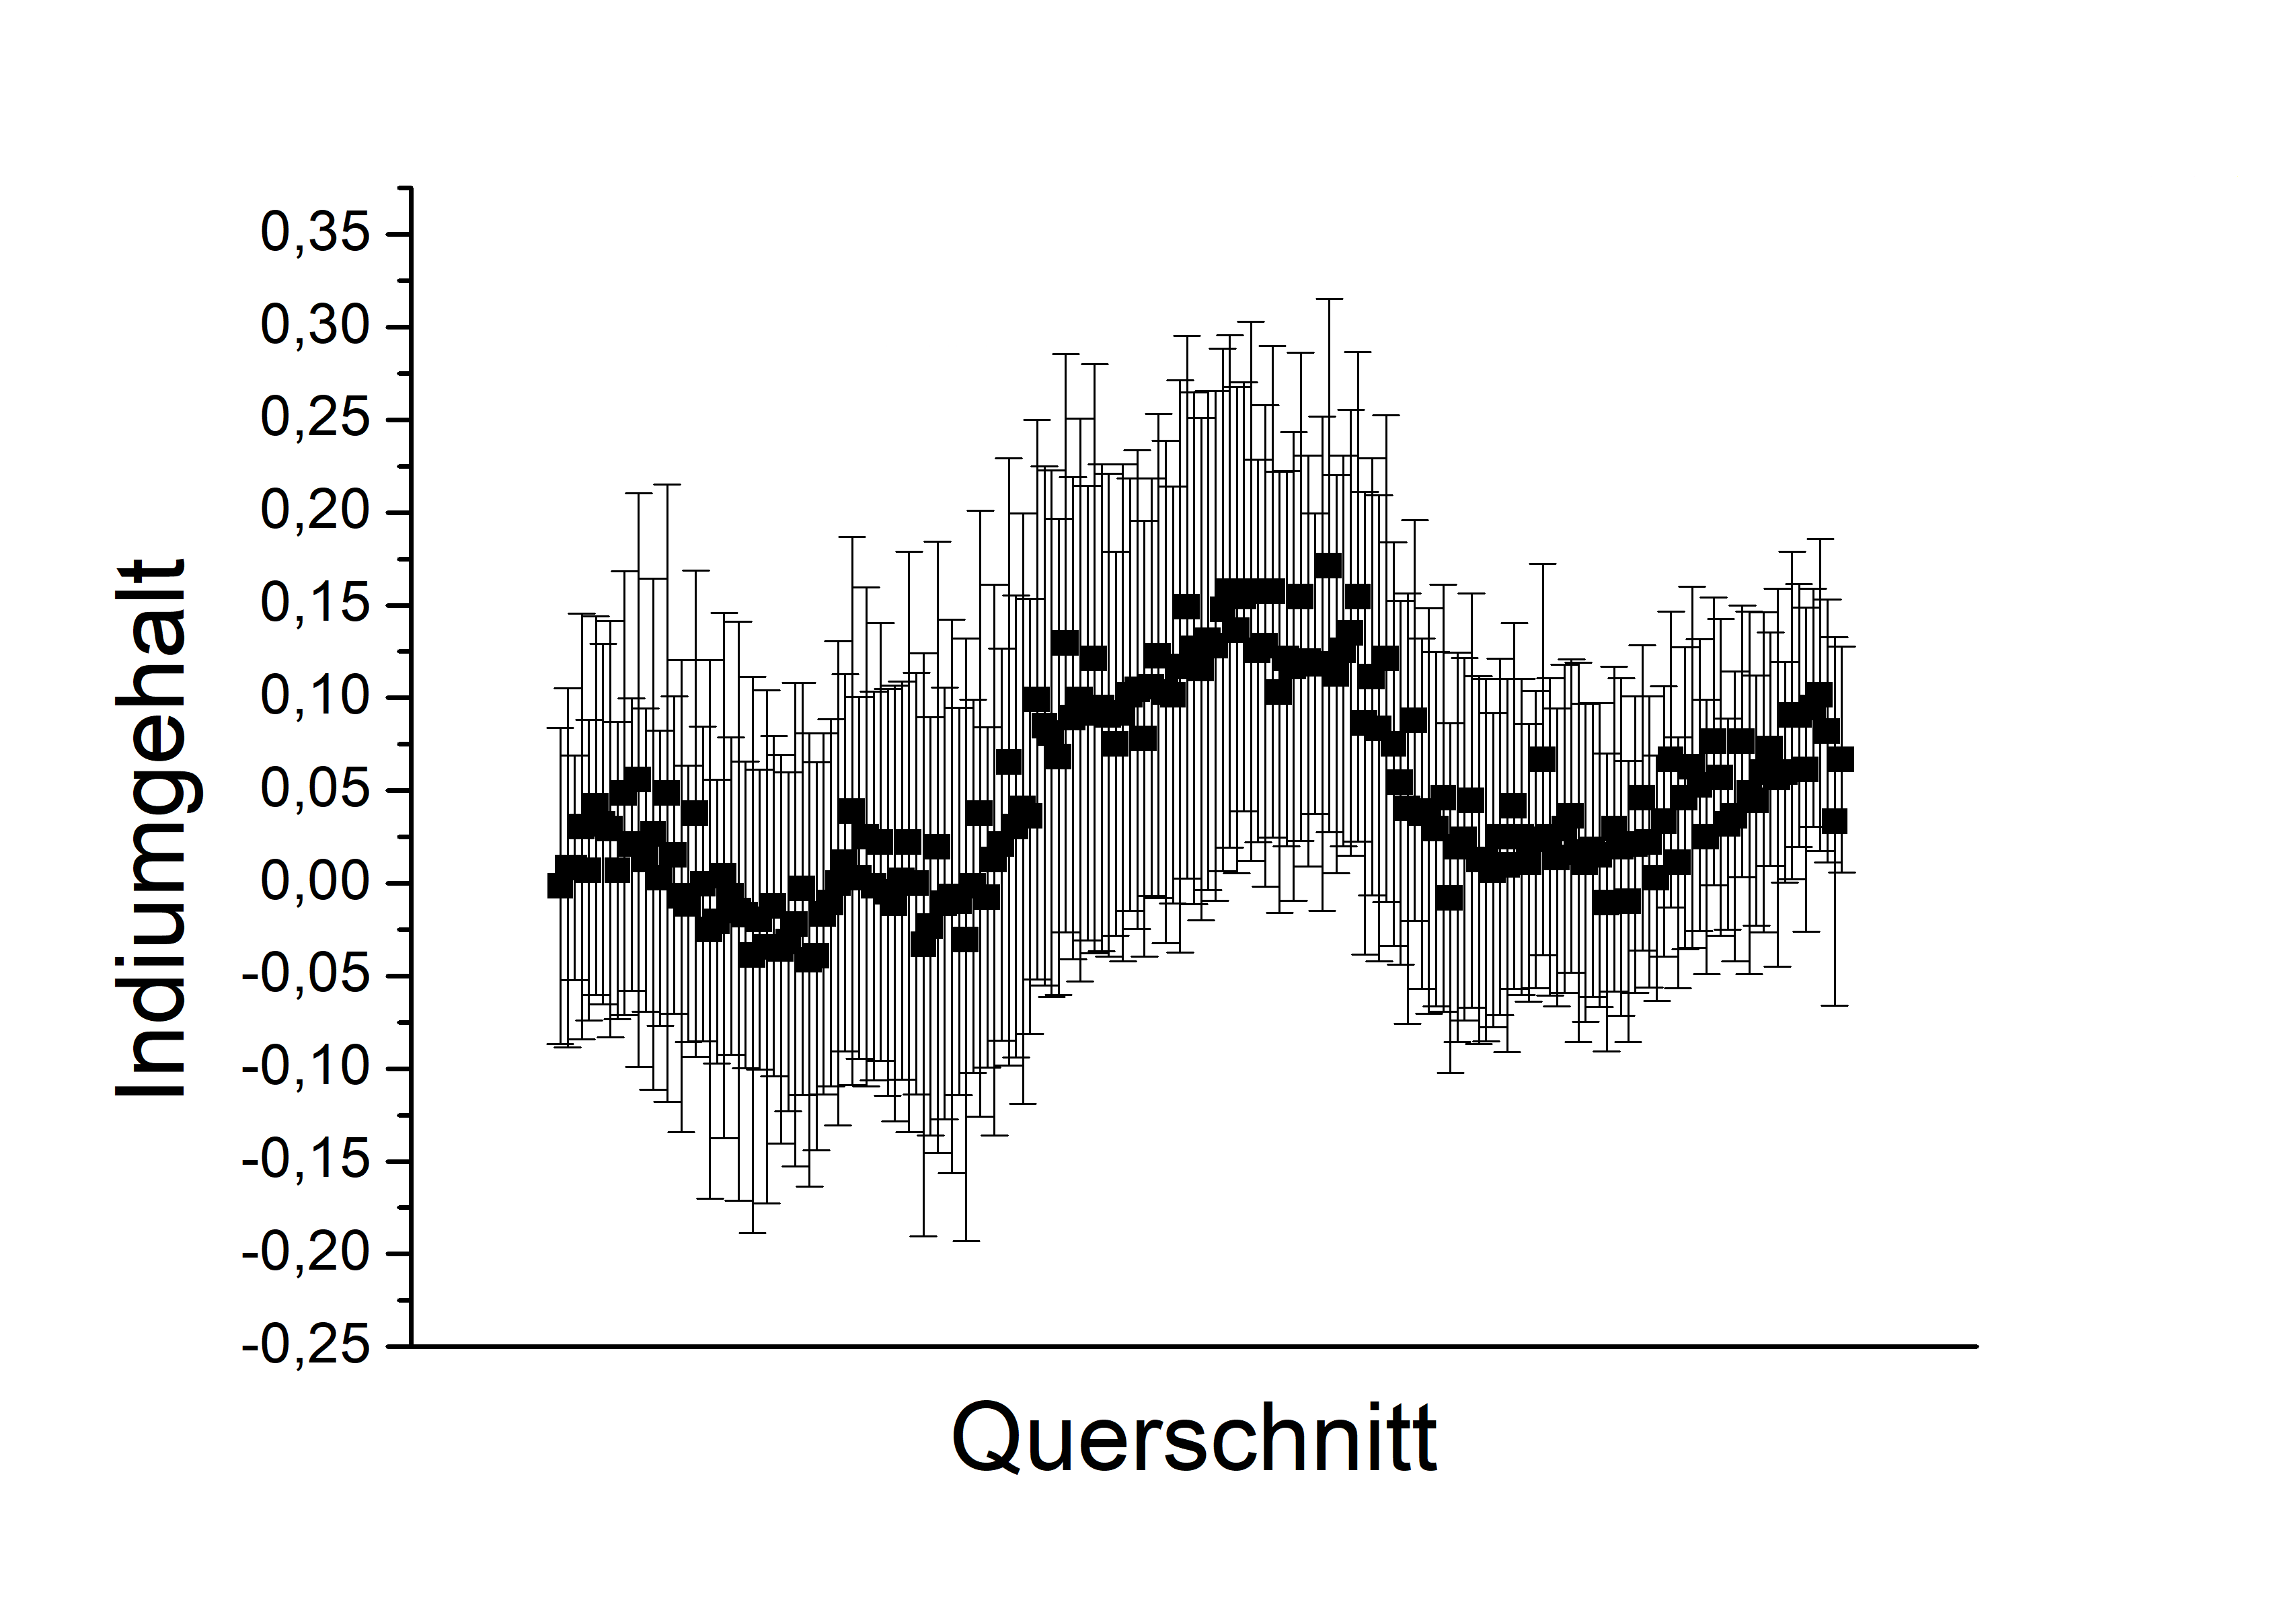
\includegraphics[width=0.9\textwidth]{Versuchsdaten/13/Graph01.png}
\caption{Profil des Indiumgehaltes, bestimmt durch die Gitterverzerrung}
\label{hochindium}
\end{figure}

Da es sich hierbei jedoch um eine andere im Vorfeld untersuchte Probe handelt, können die Ergebnisse nicht direkt miteinander verglichen werden. Der Vorteil der Gitterverzerrungs-Methode liegt allerdings darin, dass dank der höheren Auflösung die Grenzen des Quantentroges deutlich genauer zu bestimmen sind. \\
Die Fehlerbereiche der Gitterverzerrungsmethode konnten eingezeichnet werden und sind somit ersichtlich. Im Falle der Intensitäts-Methode gibt es auf den Profilen allerdings so viele Messpunkte, dass eine Darstellung der Fehlerbereiche nicht gut möglich ist. Die Fehler bewegen sich allerdings im Bereich von $\pm0,01$ bis $\pm0,02$. Hier ist allerdings eine große Unsicherheit noch nicht beachtet, da nicht fest steht, wie groß der minimale Indiumgehalt auf der Probe tatsächlich ist und durch welche andere Faktoren, wie Proben Unreinheit der Intensitätsverlauf zudem beeinflusst wird.

\section{Zusammenfassung}

In diesem Versuch konnte die Handhabung des TEM geübt und verschiedene Beugungsbilder von einer Probe gemacht werden. Durch die gezielte Drehung der Probe war es zudem möglich, Dunkelfeldaufnahmen mit den gewünschten Reflexen aufzunehmen. Beim Vergleich konnte hierbei festegestellt werden, dass Dunkelfeldaufnahmen unter bestimmten Voraussetzungen gezielt Kontraste verstärken können, sodass in diesem Fall die InGaAs-Quantentröge hervorgehoben werden konnten.
Zum Schluss konnte ein Indiumkonzentrations-Profil der Probe berechnet werden, auf dem der Verlauf um die Quantentröge herum gut sichtbar war. Hierbei wurde bestätigt, dass die Konzentrationsmessung sowohl mit der Intensität in einer Dunkelfeldaufnahme, als auch mit der Gitterverzerrung in einem Hochauflösungs-TEM Bild möglich ist. Auch die Genauigkeit ist aufgrund verschiedener Fehlerquellen bei beiden Methoden sehr ähnlich. Durch weitere Optimierung sollte, die Gitterverzerrungs-Methode allerdings eine deutlichere Zuordnung der Konzentrationen zu den Stellen auf dem Profil möglich sein, da eine höhere Auflösung als in den verwendeten Dunkelfeldbildern vorliegt.

\section*{Anhang}

\begin{figure}[htb]\centering
	\subcaptionbox{34000-fache Vergrößerung\label{34k}}
	[.49\linewidth]{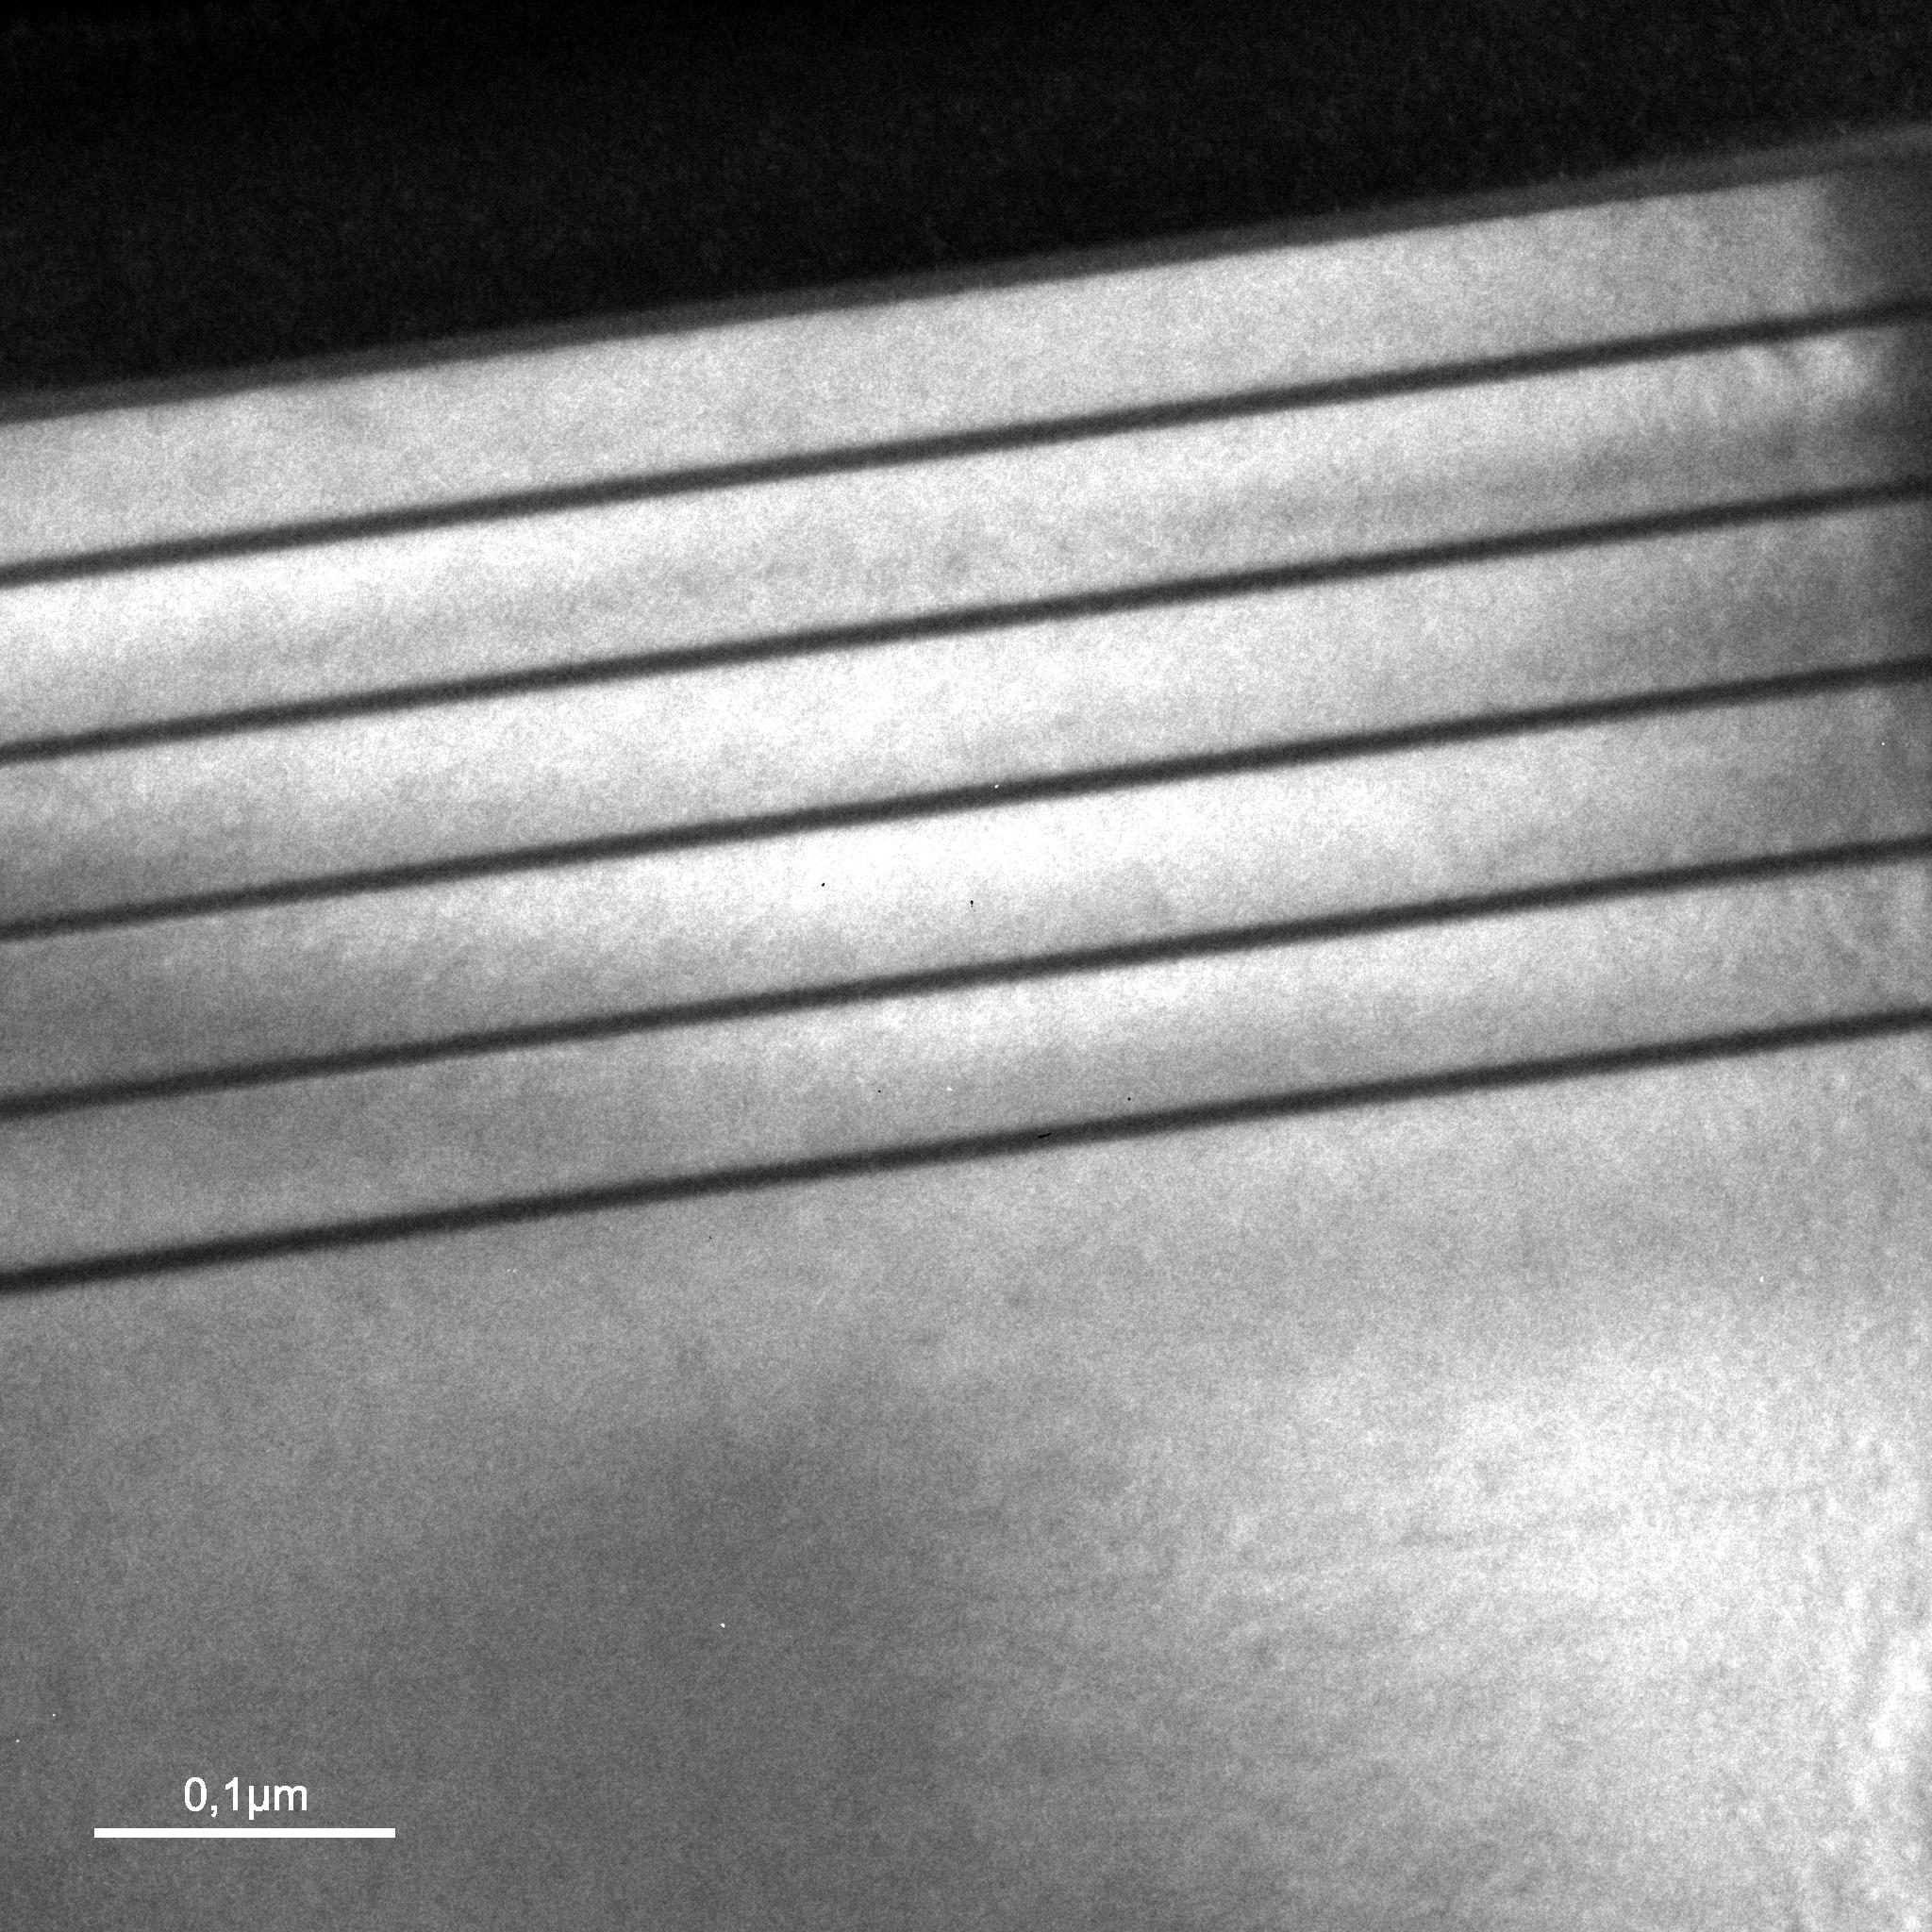
\includegraphics[width=0.49\textwidth]{Versuchsdaten/11/34000x.jpg}}
	\subcaptionbox{87000-fache Vergrößerung\label{87k}}
	[.49\linewidth]{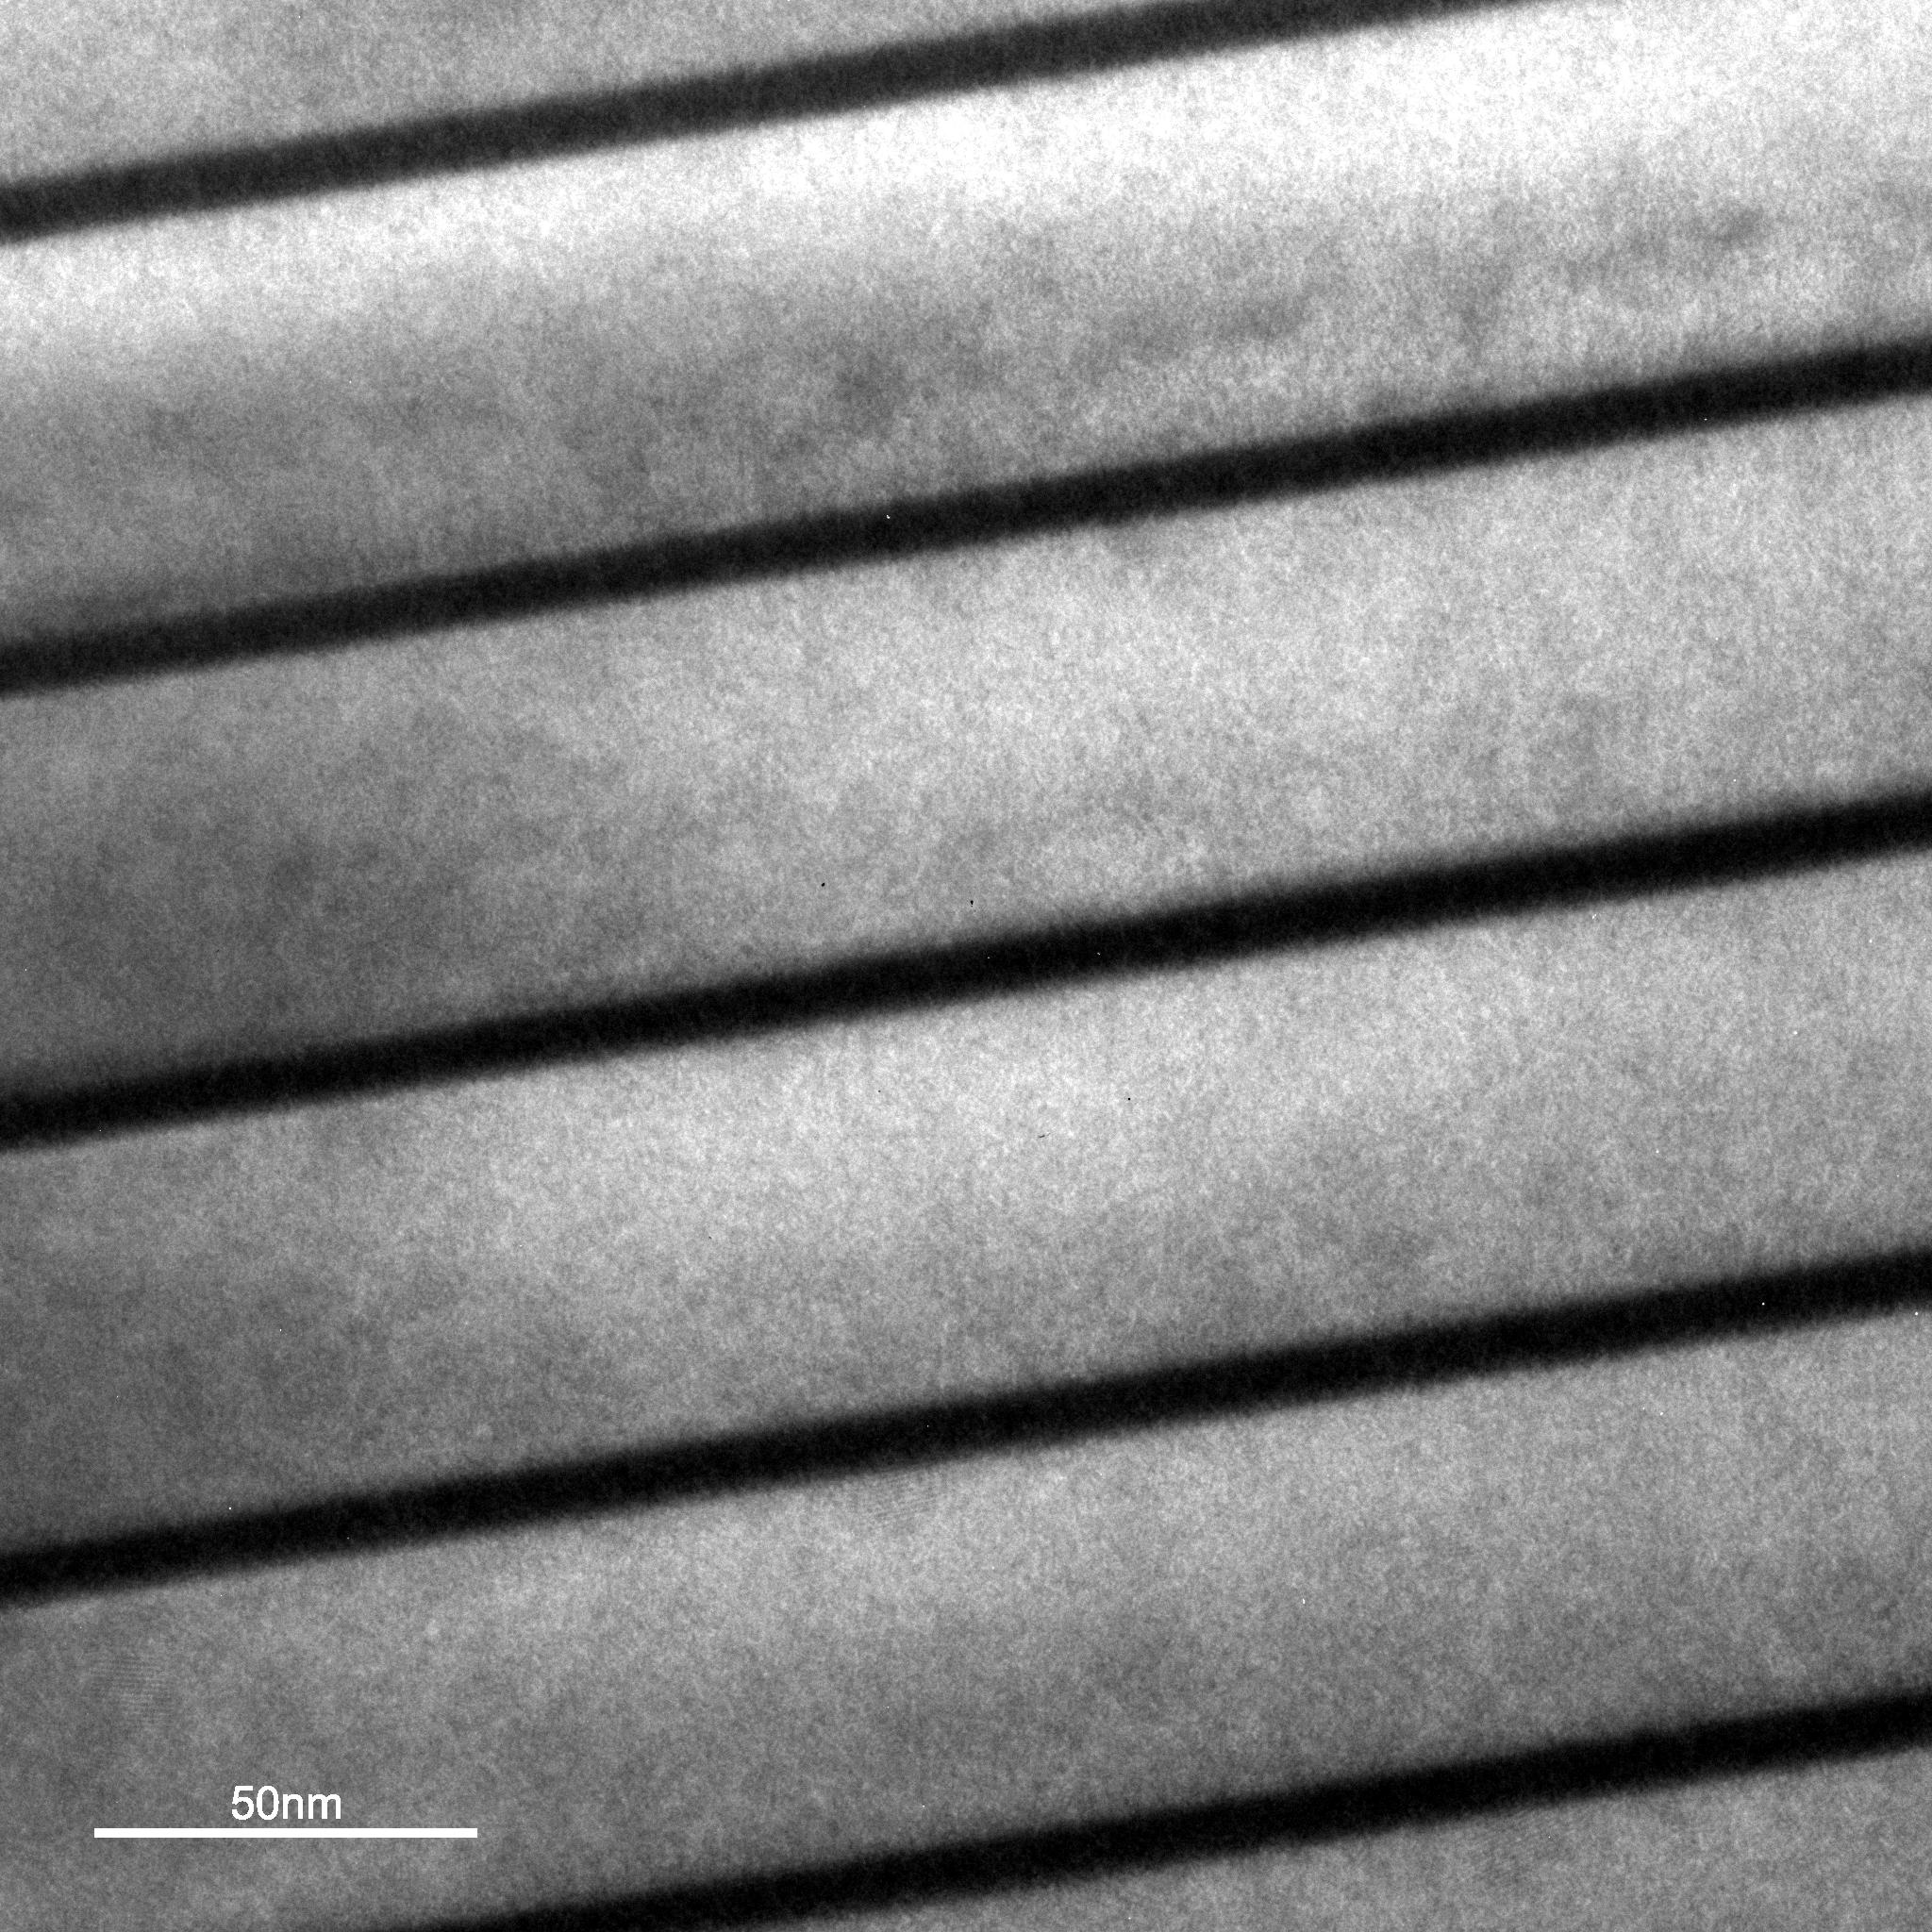
\includegraphics[width=0.49\textwidth]{Versuchsdaten/11/87000x.jpg}}\\
	\subcaptionbox{185000-fache Vergrößerung\label{185k}}
	[.49\linewidth]{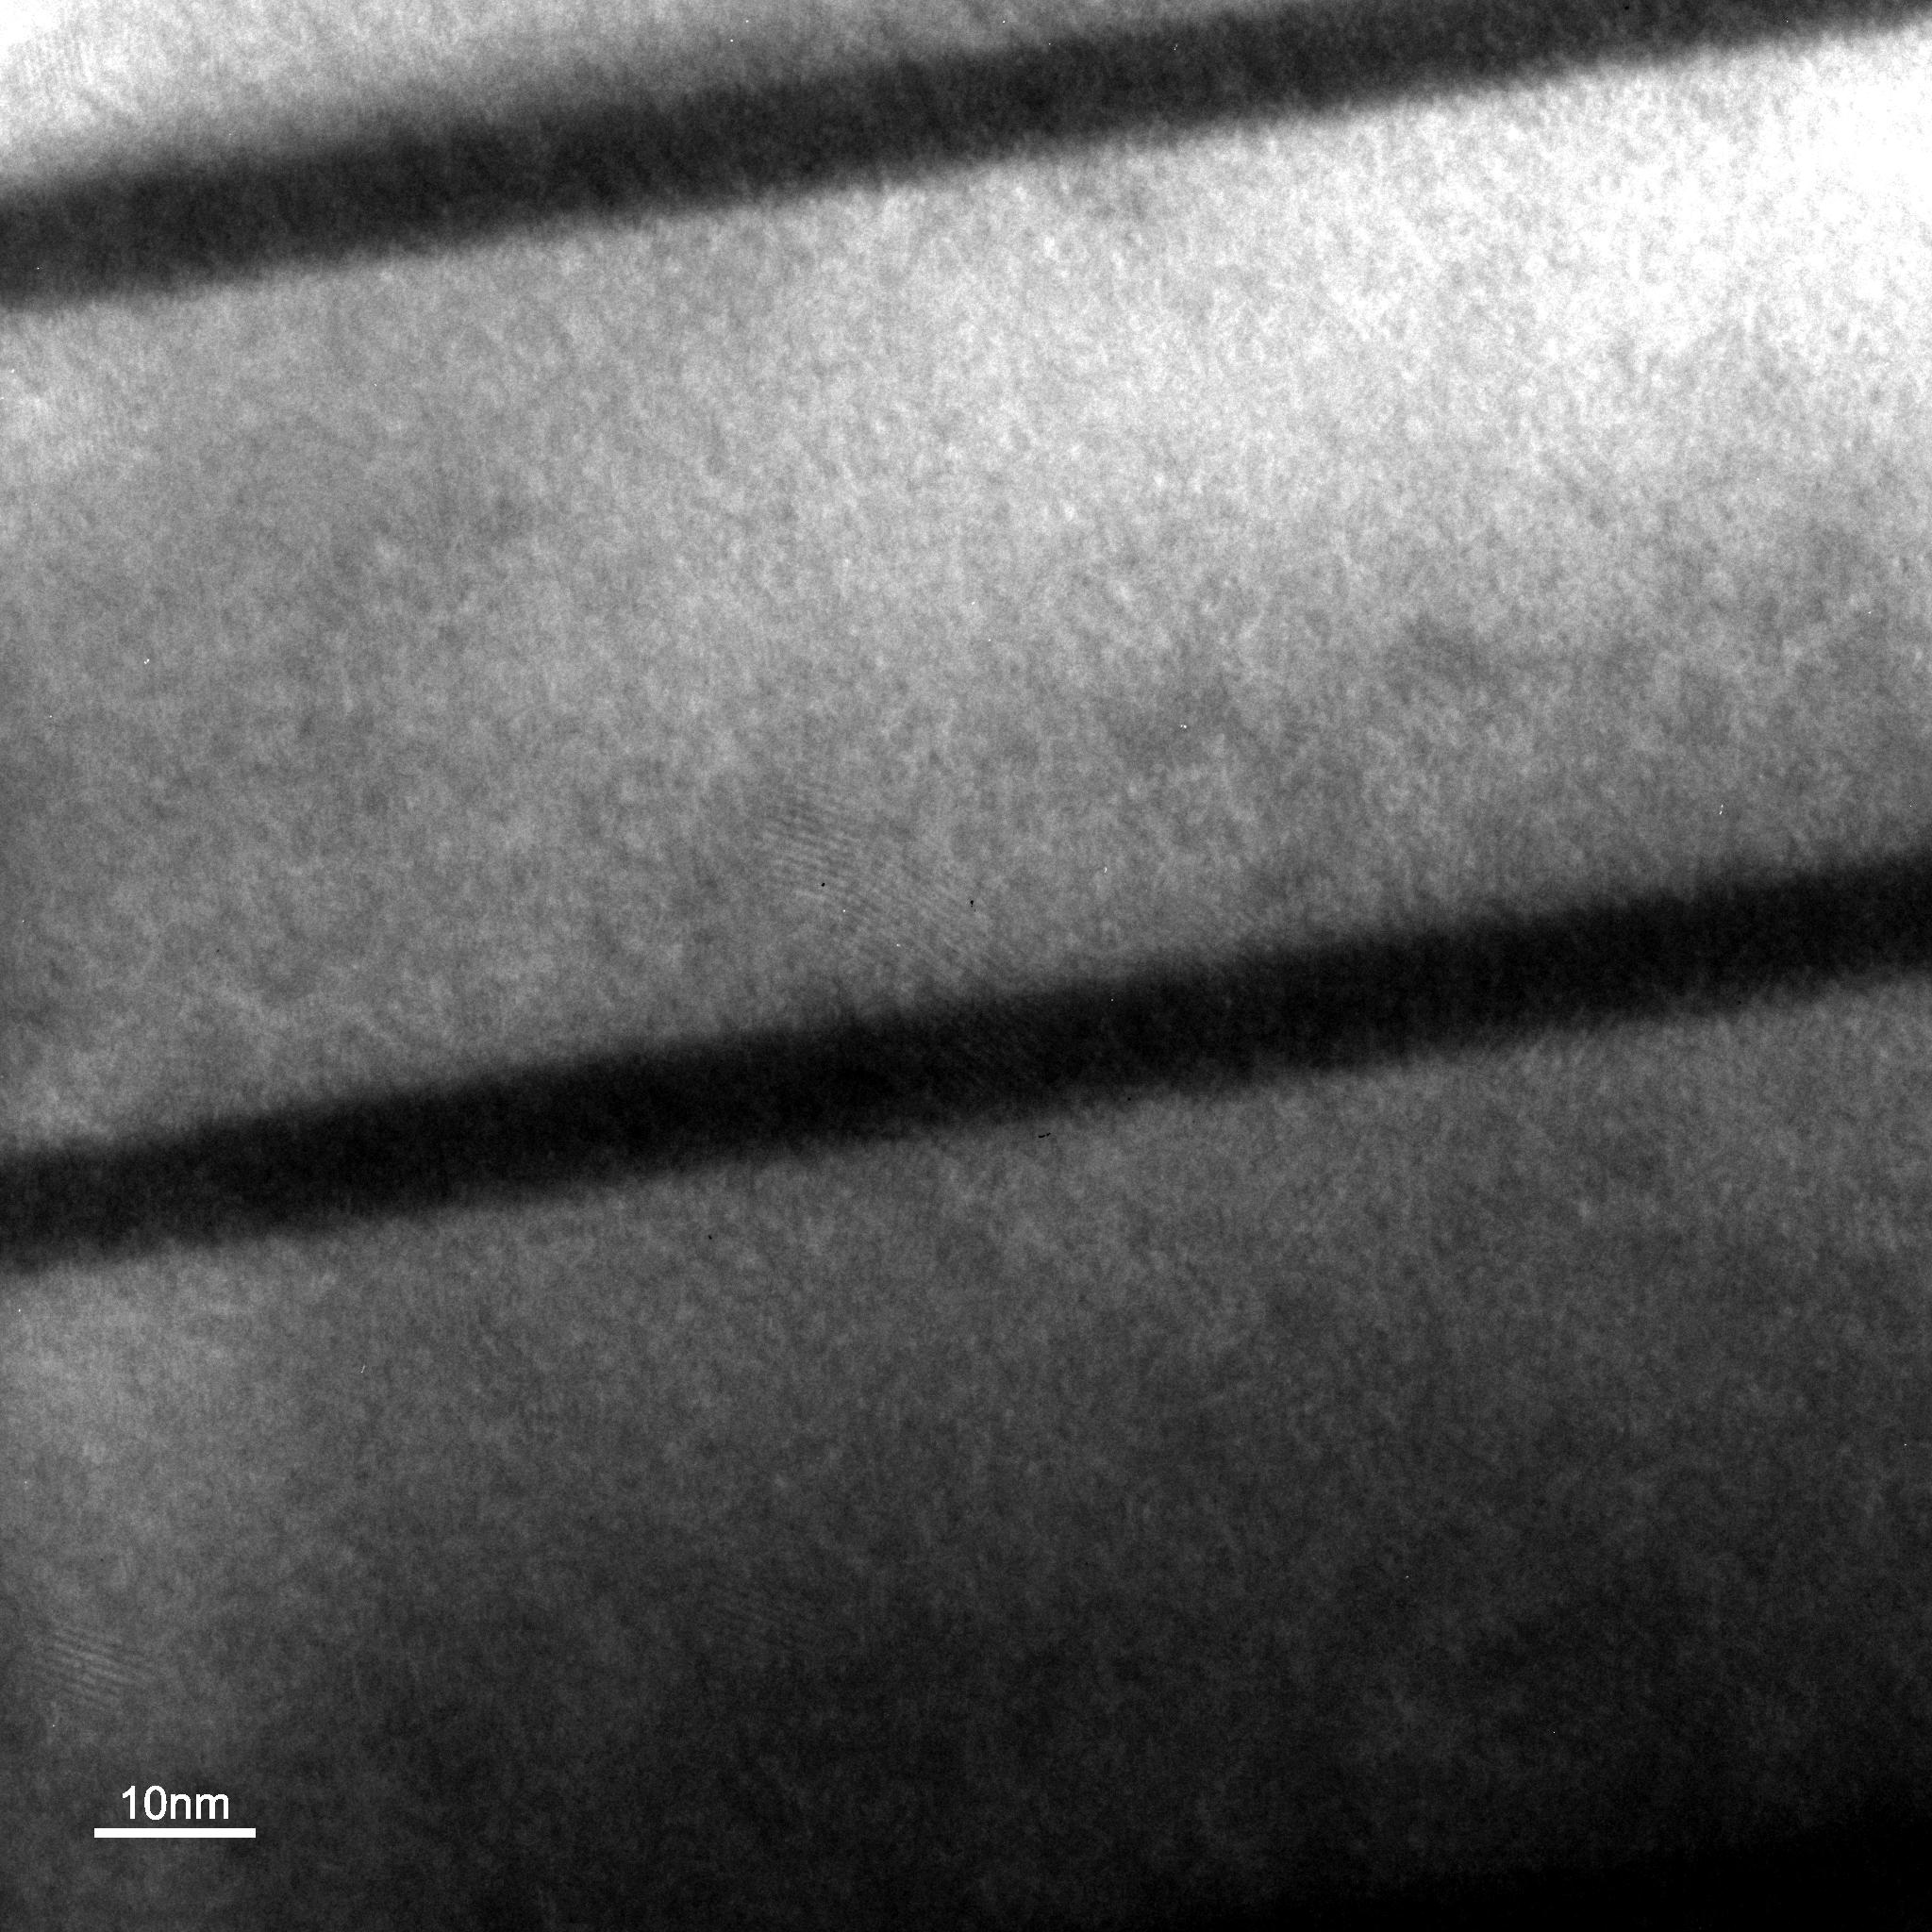
\includegraphics[width=0.49\textwidth]{Versuchsdaten/11/185000x.jpg}}
	\subcaptionbox{380000-fache Vergrößerung\label{380k}}
	[.49\linewidth]{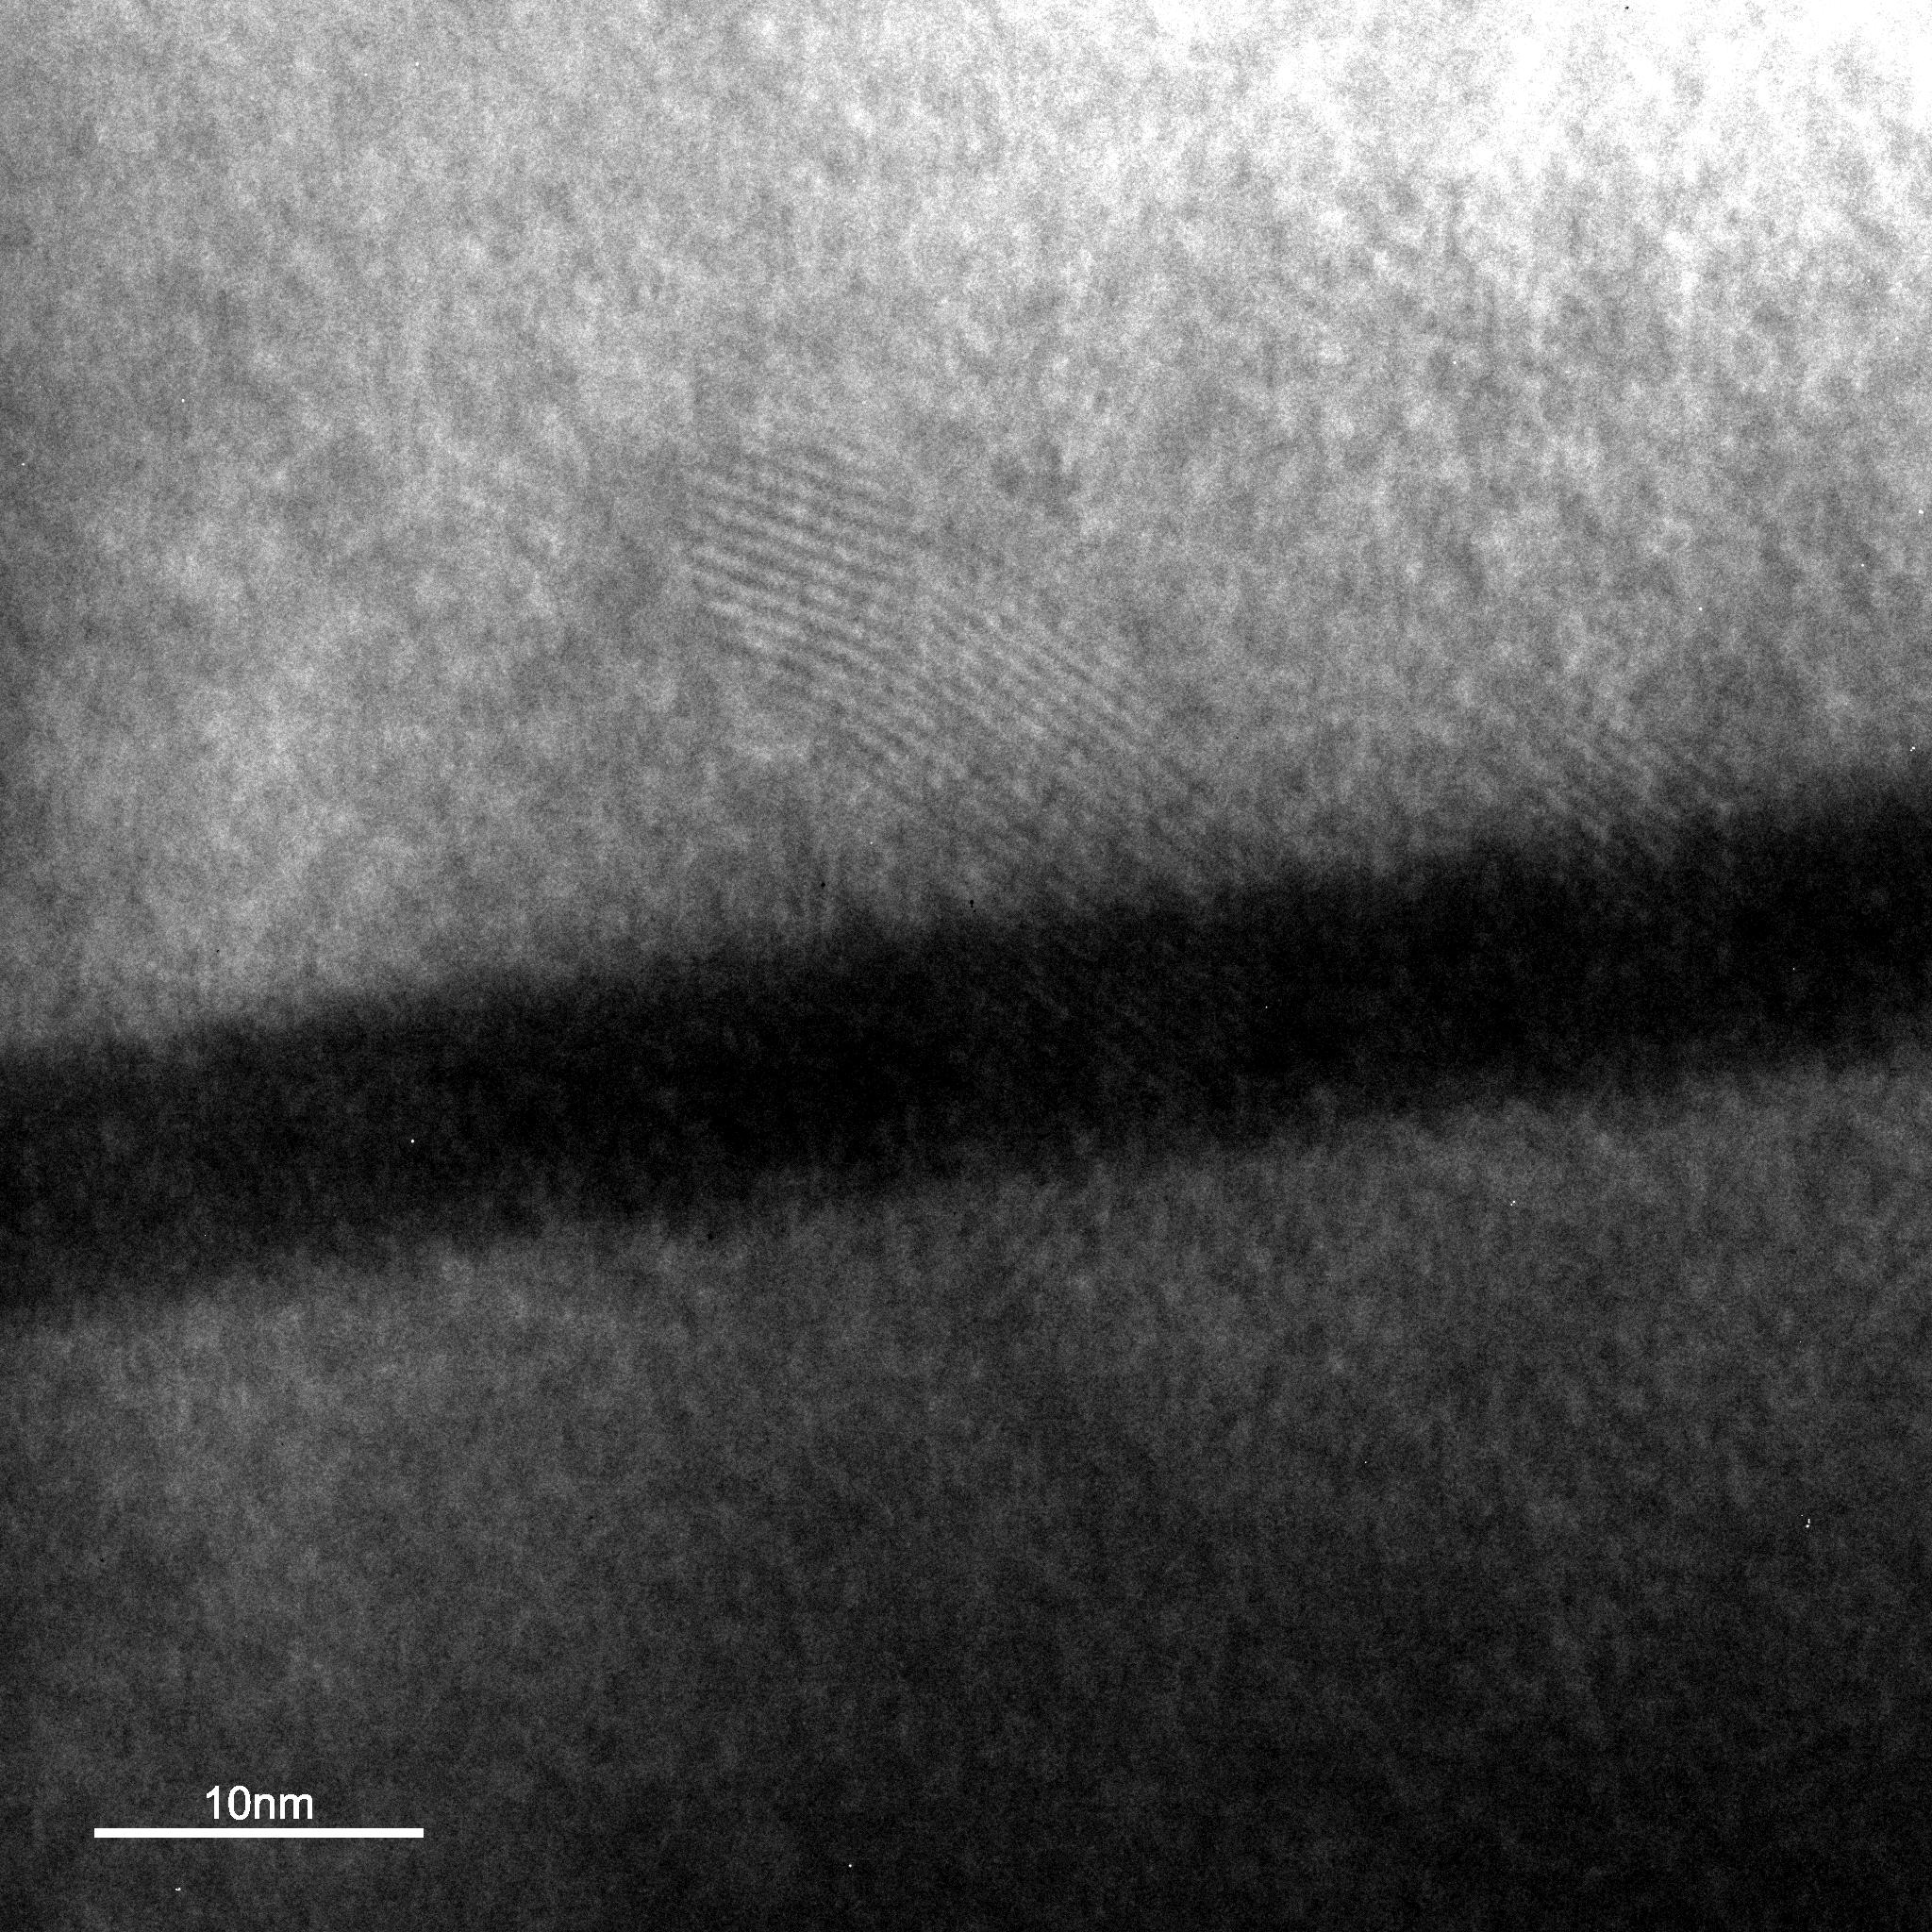
\includegraphics[width=0.49\textwidth]{Versuchsdaten/11/380000x.jpg}}
	\caption{(020) Dunkelfeldaufnahmen der InGaAs-Quantentröge mit unterschiedlichen Vergrößerungen} \label{trogdunkel}
\end{figure}

\begin{figure}[htb]\centering
	\subcaptionbox{Hochauflösungs-TEM Bild\label{hochtem}}
	[.49\linewidth]{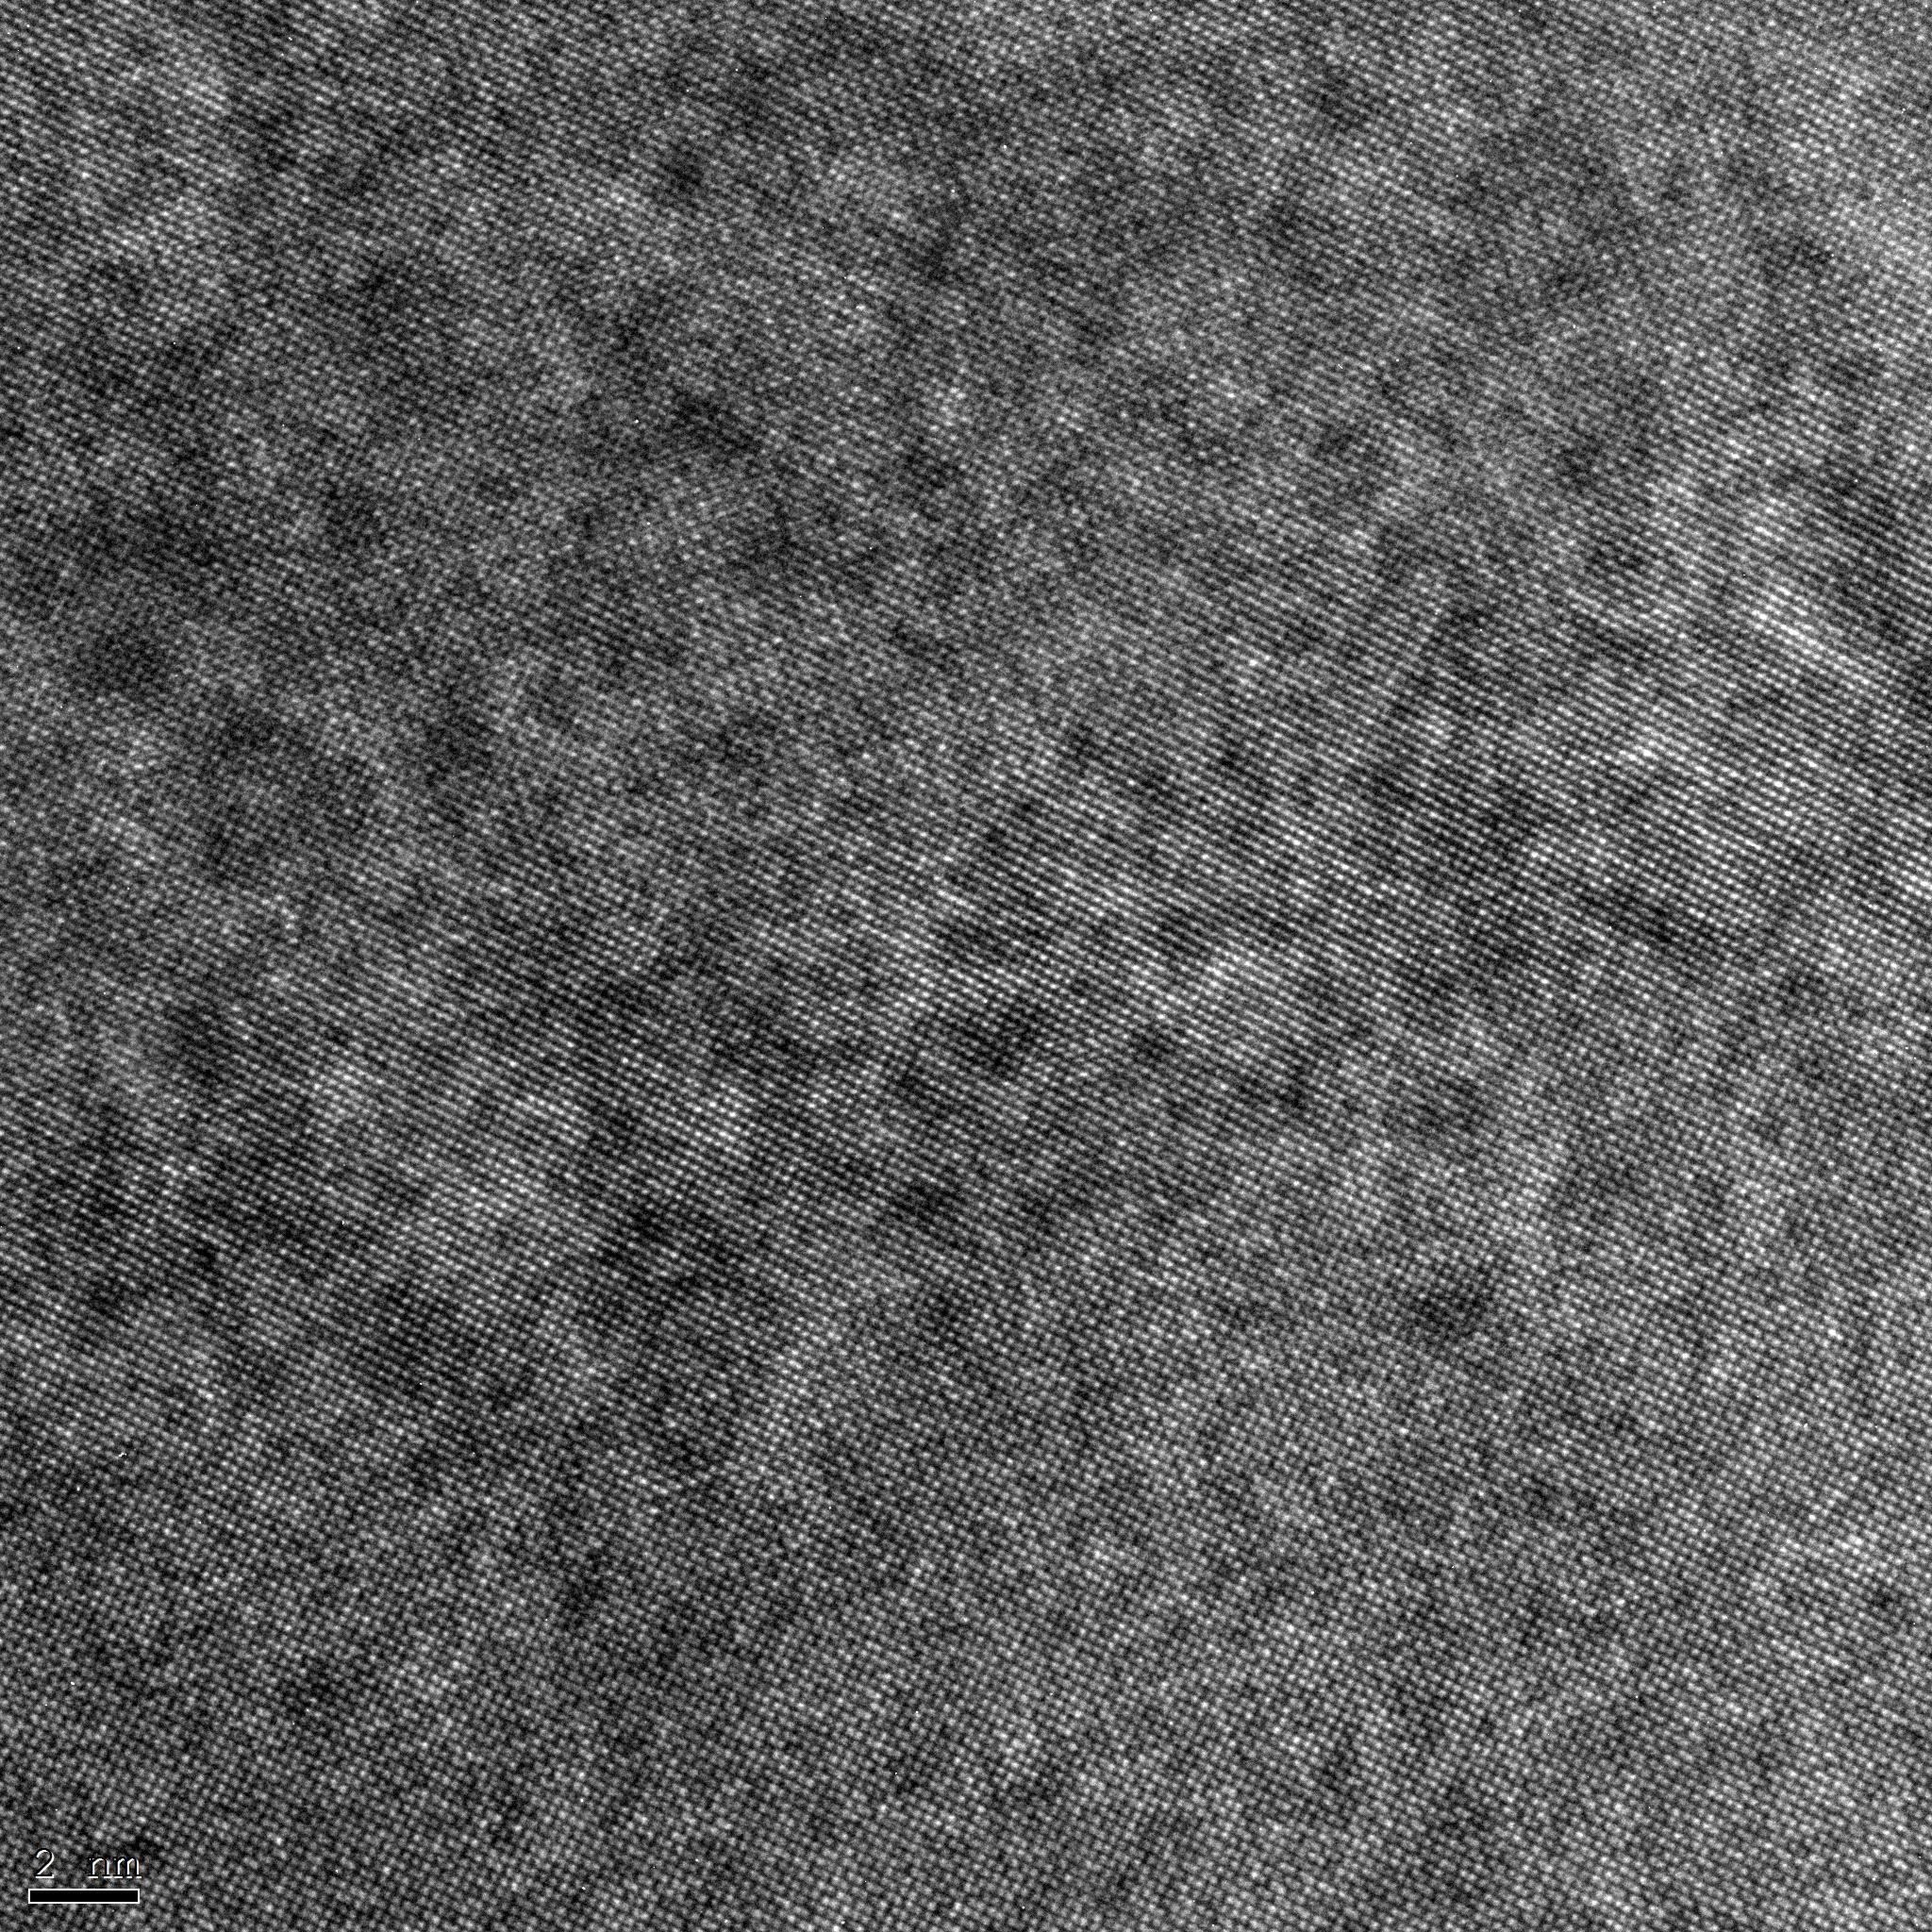
\includegraphics[width=0.49\textwidth]{Versuchsdaten/13/good_data/Frame3.jpg}}
	\subcaptionbox{Gefiltertes Bild zur Bestimmung von der Gitterkonstante\label{filthoch}}
	[.49\linewidth]{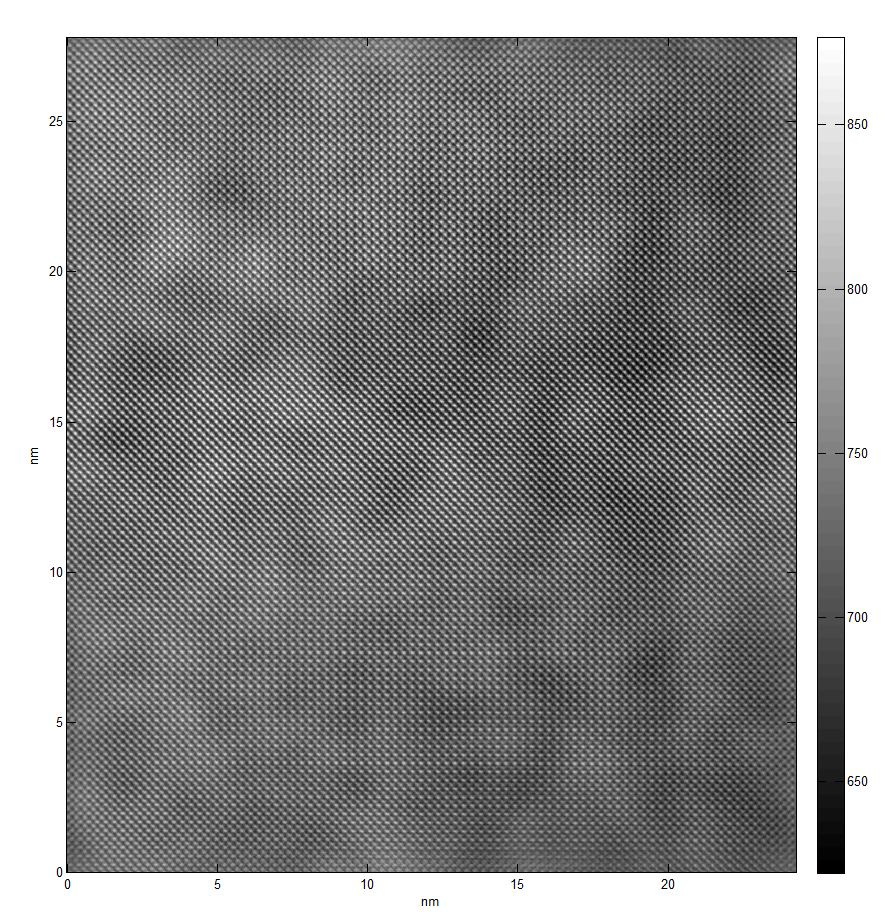
\includegraphics[width=0.49\textwidth]{Versuchsdaten/13/good_data/Frame3_rotated_and_filtered.jpg}}\\
	\caption{Hochauflösungs-TEM Bilder von InGaAs-Quantentrögen} \label{hoch}
\end{figure}

\end{document}